% Se pre-carga la información del estudiante sólo para poder emplear el macro de
% selección de versión (digital o impresa)
% ===============================================================================
% El estudiante debe llenar sus datos en esta sección para que la plantilla los 
% auto-importe y genere automáticamente las páginas de portada y de firmas 
% autorizadas.
% ===============================================================================
% Datos del estudiante:
% -------------------------------------------------------------------------------
% Nombre completo
\def \nombreestudiante {Pablo Javier \\Caal Leiva}
% Carné
\def \uvgcarne {20538}
% Facultad
\def \uvgfacultad {Ingeniería}
% Carrera
\def \uvgcarrera {Ingeniería Mecatrónica}

% Datos del trabajo:
% -------------------------------------------------------------------------------
% Título completo
\def \titulotesis {Desarrollo de herramientas de software para el control individual y seguro del cuadricóptero Crazyflie 2.1 utilizando la placa de expansión de posicionamiento con odometría visual Flow Deck}
% Año de entrega
\def \anoentrega {2024}
% Asesor
\def \nombreasesor {Msc. Miguel Zea}

% Datos del tribunal examinador:
% -------------------------------------------------------------------------------
% Nombre del primer examinador
\def \nombreprimerex {MSc. Miguel Zea}
% Nombre del segundo examinador
\def \nombresegundoex {MSc. Carlos Esquit}
% Año de aprobación
\def \anoaprobacion {2025}

% Capítulos pre-definidos
% -------------------------------------------------------------------------------
% Comentar las líneas de las secciones que desean omitirse, por defecto se 
% se incluyen todas.
\def \CAPprefacio {Prefacio}
\def \CAPantecedentes {Antecedentes}
\def \CAPalcance {Alcance}
\def \CAPanexos {Anexos}
%\def \CAPglosario {Glosario}

% Formato y estilo de la plantilla
% -------------------------------------------------------------------------------
% Modo impresión: Puede des-comentar la siguiente línea para generar un documento pdf sin la portada, para cuando se desee imprimir el documento para encuadernación
%\def \printver {Versión del documento para impresión}

% Portada: Puede cambiarse la imagen en la portada al cambiar el nombre del 
% archivo siguiente. NOTA: debe tener la suficiente resolución para cubrir el área
% designada
\def \imagenportada {plantilla/portadacit.jpg}

% Referencias: Puede des-comentar la siguiente línea para utilizar el formato de referencias APA
%\def \usarAPA {Usar formato APA}

% Párrafo: Puede comentar la siguiente línea si desea emplear un formato de 
% párrafo distinto al establecido por defecto
\def \parpordefecto {Formato de párrafo por defecto}

% Capítulos y secciones: Puede des-comentar la siguiente línea para establecer el
% formato de los capítulos y secciones bajo el estándar original de UVG para
% trabajos de graduación. Este incluye: capítulos con numeración romana, secciones
% con letras mayúsculas, sub-secciones con números y sub-sub-secciones con letras
% minúsculas
%\def \capsecuvg {Formato UVG para capítulos y secciones}

\ifdefined\printver
    \documentclass[11pt, letterpaper, twoside, openright]{report}
\else
    \documentclass[11pt, letterpaper]{report}
\fi

% Eliminar la opción de twoside y openright si se desea generar la versión
% digital del documento en lugar de la versión impresa
%\documentclass[11pt, letterpaper, twoside, openright]{report}
\usepackage[spanish, es-nodecimaldot, es-noquoting]{babel}
% cambiar a spanish, mexico si se quiere emplear tabla en lugar de cuadro
\selectlanguage{spanish}
\usepackage[utf8]{inputenc}
\usepackage[T1]{fontenc}

\title{}
\author{MSc. Miguel Zea}
\date{\today}

% Información del estudiante en el archivo datos_estudiante.tex
% ===============================================================================
% El estudiante debe llenar sus datos en esta sección para que la plantilla los 
% auto-importe y genere automáticamente las páginas de portada y de firmas 
% autorizadas.
% ===============================================================================
% Datos del estudiante:
% -------------------------------------------------------------------------------
% Nombre completo
\def \nombreestudiante {Pablo Javier \\Caal Leiva}
% Carné
\def \uvgcarne {20538}
% Facultad
\def \uvgfacultad {Ingeniería}
% Carrera
\def \uvgcarrera {Ingeniería Mecatrónica}

% Datos del trabajo:
% -------------------------------------------------------------------------------
% Título completo
\def \titulotesis {Desarrollo de herramientas de software para el control individual y seguro del cuadricóptero Crazyflie 2.1 utilizando la placa de expansión de posicionamiento con odometría visual Flow Deck}
% Año de entrega
\def \anoentrega {2024}
% Asesor
\def \nombreasesor {Msc. Miguel Zea}

% Datos del tribunal examinador:
% -------------------------------------------------------------------------------
% Nombre del primer examinador
\def \nombreprimerex {MSc. Miguel Zea}
% Nombre del segundo examinador
\def \nombresegundoex {MSc. Carlos Esquit}
% Año de aprobación
\def \anoaprobacion {2025}

% Capítulos pre-definidos
% -------------------------------------------------------------------------------
% Comentar las líneas de las secciones que desean omitirse, por defecto se 
% se incluyen todas.
\def \CAPprefacio {Prefacio}
\def \CAPantecedentes {Antecedentes}
\def \CAPalcance {Alcance}
\def \CAPanexos {Anexos}
%\def \CAPglosario {Glosario}

% Formato y estilo de la plantilla
% -------------------------------------------------------------------------------
% Modo impresión: Puede des-comentar la siguiente línea para generar un documento pdf sin la portada, para cuando se desee imprimir el documento para encuadernación
%\def \printver {Versión del documento para impresión}

% Portada: Puede cambiarse la imagen en la portada al cambiar el nombre del 
% archivo siguiente. NOTA: debe tener la suficiente resolución para cubrir el área
% designada
\def \imagenportada {plantilla/portadacit.jpg}

% Referencias: Puede des-comentar la siguiente línea para utilizar el formato de referencias APA
%\def \usarAPA {Usar formato APA}

% Párrafo: Puede comentar la siguiente línea si desea emplear un formato de 
% párrafo distinto al establecido por defecto
\def \parpordefecto {Formato de párrafo por defecto}

% Capítulos y secciones: Puede des-comentar la siguiente línea para establecer el
% formato de los capítulos y secciones bajo el estándar original de UVG para
% trabajos de graduación. Este incluye: capítulos con numeración romana, secciones
% con letras mayúsculas, sub-secciones con números y sub-sub-secciones con letras
% minúsculas
%\def \capsecuvg {Formato UVG para capítulos y secciones}
% ================================================================================
% En este archivo se colocan opciones adicionales para modificar el formato de la
% plantilla, para emplearse en otros tipos de documentos que no sean trabajos de
% graduación. Si usted está trabajando su tesis, NO modifique este archivo
% ================================================================================
% Capítulos pre-definidos
% --------------------------------------------------------------------------------
% Comentar las líneas de las secciones que desean omitirse, por defecto se 
% se incluyen todas.
\def \CAPportada {Portada}
\def \CAPcaratula {Caratula}
\def \CAPfirmas {Hoja de firmas}
\def \CAPindice {Índice general}
\def \CAPfiguras {Listado de figuras}
\def \CAPcuadros {Listado de cuadros}
\def \CAPresumen {Resumen}
\def \CAPabstract {Resumen}
\def \CAPintroduccion {Introducción}
\def \CAPobjetivos {Objetivos}
\def \CAPjustificacion {Justificación}
\def \CAPmarcoteorico {Marco teórico}
\def \CAPconclusiones {Conclusiones}
\def \CAPrecomendaciones {Recomendaciones}
\def \CAPbibliografia {Bibliografía}

% ==============================================================================
% DEFINICIÓN DE PAQUETES
% ==============================================================================
\usepackage{xcolor}
\usepackage{amsfonts}
\usepackage{amsmath}
\usepackage{amssymb}
\usepackage{amsthm}
\usepackage{amsfonts}
\usepackage{mathtools}
\usepackage{graphicx}
\usepackage{xfrac}
\usepackage{float}
\usepackage{mathtools}
\usepackage[hypertexnames=false]{hyperref}
% \usepackage{bookmark}
\usepackage[font=small]{caption}
\usepackage{subcaption}
%\usepackage{csquotes}
\usepackage{xpatch}
\usepackage{emptypage}
\usepackage{hyphenat}
\usepackage{fancyhdr}
\usepackage[backend=biber, style=ieee]{biblatex}
\ifdefined\usarAPA 
    \usepackage[backend=biber, style=apa]{biblatex}
\fi
\addbibresource{m-bibliografia.bib}

\usepackage[percent]{overpic}

\usepackage{chngcntr}
\usepackage{csquotes}

\usepackage[utf8]{inputenc}   % Asegura la codificación UTF-8
\usepackage[T1]{fontenc}      % Asegura el uso de una codificación de fuente compatible
\usepackage{listings}
\usepackage{xcolor}
\renewcommand{\lstlistingname}{Código} % Cambia 'Listing' a 'Código'
\lstset{
	inputencoding=utf8,          % Especifica la codificación de entrada como UTF-8
	extendedchars=true,          % Permite caracteres extendidos (acentos)
	literate={á}{{\'a}}1 {é}{{\'e}}1 {í}{{\'i}}1 {ó}{{\'o}}1 {ú}{{\'u}}1
	{Á}{{\'A}}1 {É}{{\'E}}1 {Í}{{\'I}}1 {Ó}{{\'O}}1 {Ú}{{\'U}}1
	{ñ}{{\~n}}1 {Ñ}{{\~N}}1 {¡}{{\textexclamdown}}1 {¿}{{\textquestiondown}}1,
	basicstyle=\ttfamily\footnotesize, % Tamaño de fuente y tipo monoespaciado
	keywordstyle=\color{blue},         % Color de las palabras clave
	stringstyle=\color{red},           % Color de las cadenas
	commentstyle=\color{gray},         % Color de los comentarios
	backgroundcolor=\color{lightgray!20}, % Color de fondo
	frame=single,                      % Coloca un marco alrededor del código
	framerule=0.5pt,                   % Grosor del marco
	rulecolor=\color{black},           % Color del marco
	breaklines=true,                   % Permite el corte de líneas largas
	captionpos=b,                      % Posición de la leyenda (caption) en la parte inferior
	showstringspaces=false,            % No mostrar los espacios en las cadenas
	numbers=left,                      % Mostrar los números de línea
	numberstyle=\tiny,                 % Tamaño de la fuente para los números de línea
	numbersep=5pt,                     % Separación de los números de línea
	tabsize=2,                         % Tamaño de tabulación
	language=sh,                       % Lenguaje del código (bash en este caso)
	escapeinside={(*@}{@*)},           % Permite la inserción de comandos LaTeX dentro del código
	xleftmargin=2em,                   % Margen izquierdo
	framexleftmargin=1.5em             % Margen del marco desde el texto
}



\ifdefined\CAPglosario
	%\usepackage[toc]{glossaries}
	\usepackage[numberedsection]{glossaries}
	\makeglossaries
    \input{o-glosario}
\fi

% ==============================================================================
% MÁRGENES Y FORMATO GENERALES
% ==============================================================================
\usepackage[top=1in, left=1.5in, right=1in, bottom=1in]{geometry}
%Options: Sonny, Lenny, Glenn, Conny, Rejne, Bjarne, Bjornstrup
\usepackage[Sonny]{fncychap}

% ==============================================================================
% DEFINICIONES DE LA PLANTILLA
% ==============================================================================
\graphicspath{ {figuras/} }
\definecolor{uvg-green}{RGB}{17,71,52}
\newcommand{\defaultparformat}[1]{
	{\setlength{\parskip}{2ex}
     \input{#1}}
}
\ifdefined\capsecuvg
	\renewcommand\thechapter{\Roman{chapter}}
    \renewcommand\thesection{\Alph{section}}
	\renewcommand\thesubsection{\arabic{subsection}}
    \renewcommand\thesubsubsection{\alph{subsubection}}
\fi
\counterwithout{figure}{chapter}
\counterwithout{table}{chapter}
\counterwithout{equation}{chapter}

\newcommand{\blankpage}{
\newpage
\thispagestyle{empty}
\mbox{}
\newpage
}
% ==============================================================================

% Comandos definidos por el usuario en el archivo comandos_usuario.tex
\input{2-paquetes_y_comandos_usuario}

% ==============================================================================
% CUERPO DEL TRABAJO
% ==============================================================================
\pagestyle{headings}
\begin{document}

% ==============================================================================
% PORTADA
% ==============================================================================
\ifdefined\printver
    \let\CAPportada\undefined
\fi 

\ifdefined\CAPportada
    \cleardoublepage\phantomsection
    % \pdfbookmark{Portada}{toc}
	\newgeometry{left=3cm, bottom=0in, top=1in, right=3cm}
	\pagecolor{uvg-green}
	\thispagestyle{empty}

	\color{white}
	\noindent \hrulefill \par
	\vspace{0.1in}
	\noindent \Huge \nohyphens{\titulotesis} \par
	\noindent \hrulefill \par
	\noindent
	\LARGE \nombreestudiante

	\begin{figure}[b!]
    	%\makebox[\textwidth]{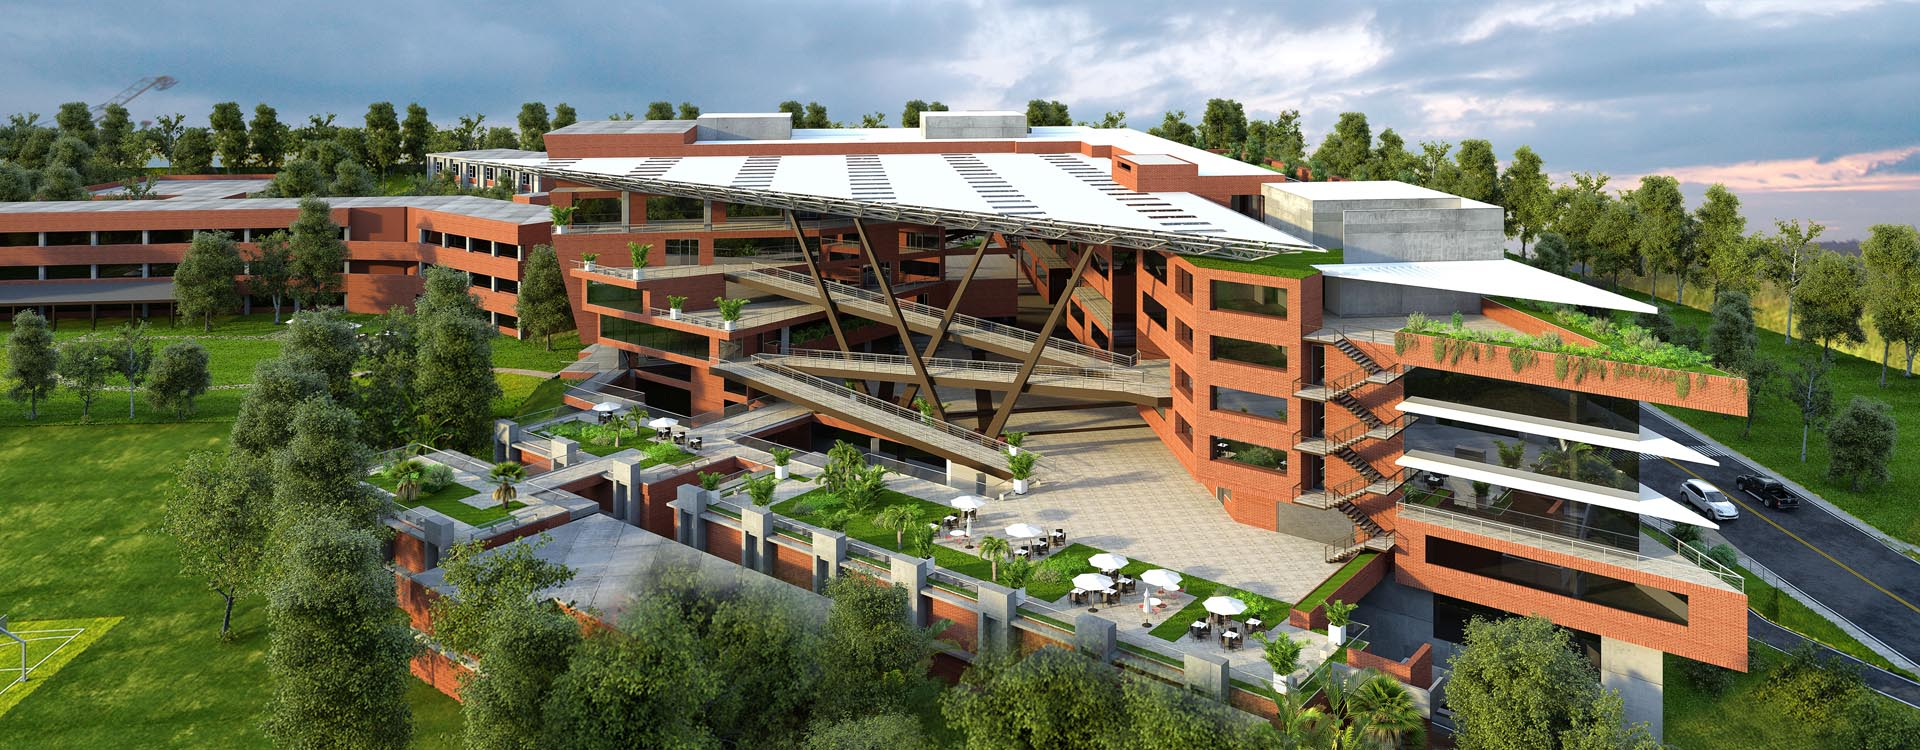
\includegraphics[height=13.25cm]{plantilla/portadacit.jpg}}
    	\makebox[\textwidth]{
    		\begin{overpic}[height=13.25cm]{\imagenportada}
     		\put(63,0){
\includegraphics[height=1.15in]{plantilla/fondologo_grande.png}}  
  			\put(64.5,2){
\includegraphics[height=0.55in]{plantilla/logoUVGblanco.eps}} 
        	\end{overpic}
    	}
    	%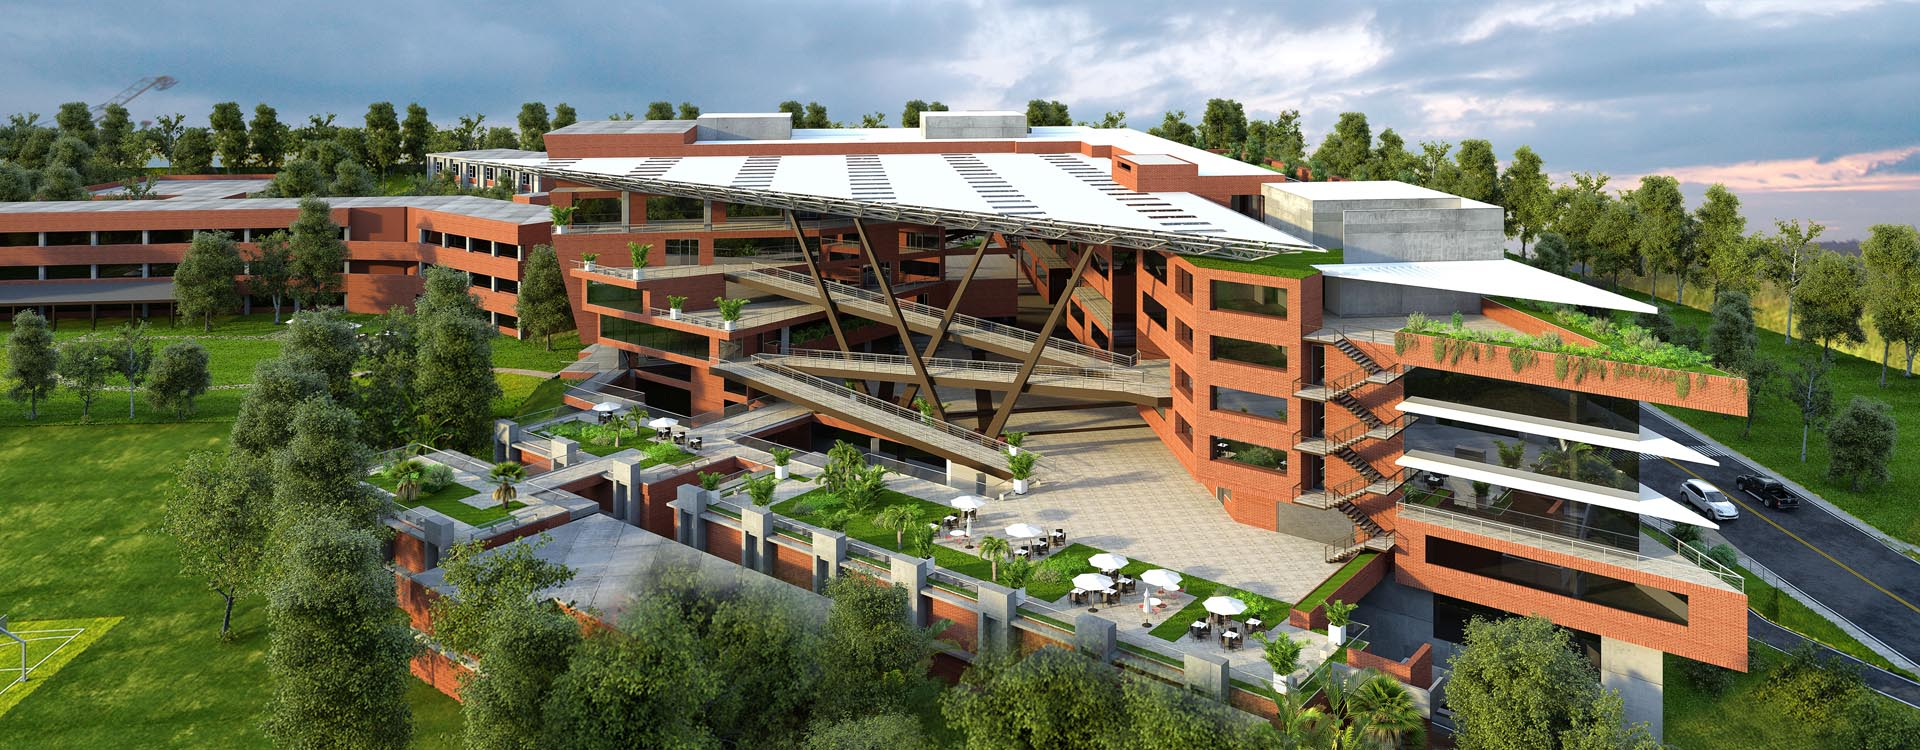
\includegraphics[height=13.25cm]{plantilla/portadacit.jpg}
	\end{figure}
	\restoregeometry
\fi

% ==============================================================================
% PRIMERAS PÁGINAS (Carátulas más hojas de guarda)
% ==============================================================================
\ifdefined\CAPcaratula
	\newpage
    \cleardoublepage\phantomsection
    % \pdfbookmark{Carátula}{toc}
	\pagecolor{white}
	\color{black}
	\setcounter{page}{1}
	\pagenumbering{roman}
	\thispagestyle{empty}
	\begin{center}
		\LARGE UNIVERSIDAD DEL VALLE DE GUATEMALA\\
		\LARGE Facultad de \uvgfacultad \\[0.75cm]
	\end{center}
	\begin{figure}[h]
		\begin{center}
		
\includegraphics[height=5.5 cm]{plantilla/escudoUVGnegro.eps}
		\vspace{0.5in}
		\end{center}
	\end{figure}
	\begin{center}
		\Large \textbf{\nohyphens{\titulotesis}} \\
		%\LARGE \textbf{\titulotesis} \\
		\vfill
		\Large \nohyphens{Trabajo de graduación presentado por \nombreestudiante \ para optar al grado académico de Licenciado en \uvgcarrera} \\
		\vfill
		\large Guatemala, \\
		\vspace{1em}
		\anoentrega
	\end{center}
    
    \ifdefined\printver	
	    \blankpage
	    \blankpage
	    
	    \newpage
	    \cleardoublepage\phantomsection
	    \pagecolor{white}
    	\color{black}
    	\setcounter{page}{1}
    	\pagenumbering{roman}
    	\thispagestyle{empty}
    	\begin{center}
    		\LARGE UNIVERSIDAD DEL VALLE DE GUATEMALA\\
    		\LARGE Facultad de \uvgfacultad \\[0.75cm]
    	\end{center}
    	\begin{figure}[h]
    		\begin{center}
    		
\includegraphics[height=5.5 cm]{plantilla/escudoUVGnegro.eps}
    		\vspace{0.5in}
    		\end{center}
    	\end{figure}
    	\begin{center}
    		\Large \textbf{\nohyphens{\titulotesis}} \\
    		%\LARGE \textbf{\titulotesis} \\
    		\vfill
    		\Large \nohyphens{Trabajo de graduación presentado por \nombreestudiante \ para optar al grado académico de Licenciado en \uvgcarrera} \\
    		\vfill
    		\large Guatemala, \\
    		\vspace{1em}
    		\anoentrega
    	\end{center}
    \fi
\fi

% ==============================================================================
% HOJA DE FIRMAS
% ==============================================================================
\ifdefined\CAPfirmas
	\newpage
	\cleardoublepage\phantomsection
	\thispagestyle{empty}
	\vspace*{0.5in}
	\large Vo.Bo.:\\[1cm]
	\begin{center}
		(f) \rule[1pt]{4 in}{1pt}\\
		\nombreasesor
	\end{center}
	\vspace{1in}

	Tribunal Examinador:\\[1cm]
	\begin{center}
		(f) \rule[1pt]{4 in}{1pt}\\
		\nombreasesor \\[1in]
		(f) \rule[1pt]{4 in}{1pt}\\
		\nombreprimerex \\[1in]
		(f) \rule[1pt]{4 in}{1pt}\\
		\nombresegundoex
	\end{center}
	\vspace{1in}

%	Fecha de aprobación: Guatemala, \rule[1pt]{0.5 in}{1pt} de \rule[1pt]{1 in}{1pt} de \anoaprobacion.
    Fecha de aprobación: Guatemala, \diaaprobacion de \mesaprobacion de \anoaprobacion.
	\normalsize
\fi

% Comentar para formato estilo libro en la numeración de páginas (NO 
% compatible con la guía UVG 2019)
\pagestyle{plain}
% ==============================================================================
% CONTENIDO DEL TRABAJO
% ==============================================================================
% PREFACIO
% ------------------------------------------------------------------------------
\ifdefined\CAPprefacio
	\newpage
	\cleardoublepage\phantomsection
    \chapter*{Prefacio}
    \ifdefined\parpordefecto
    	\defaultparformat{a-prefacio}
    \else
    	Lorem ipsum dolor sit amet, consectetur adipiscing elit. Cras vitae eleifend ipsum, ut mattis nunc. Pellentesque ac hendrerit lacus. Cras sollicitudin eget sem nec luctus. Vivamus aliquet lorem id elit venenatis pellentesque. Nam id orci iaculis, rutrum ipsum vel, porttitor magna. Etiam molestie vel elit sed suscipit. Proin dui risus, scelerisque porttitor cursus ac, tempor eget turpis. Aliquam ultricies congue ligula ac ornare. Duis id purus eu ex pharetra feugiat. Vivamus ac orci arcu. Nulla id diam quis erat rhoncus hendrerit. Class aptent taciti sociosqu ad litora torquent per conubia nostra, per inceptos himenaeos. Sed vulputate, metus vel efficitur fringilla, orci ex ultricies augue, sit amet rhoncus ex purus ut massa. Nam pharetra ipsum consequat est blandit, sed commodo nunc scelerisque. Maecenas ut suscipit libero. Sed vel euismod tellus.

Proin elit tellus, finibus et metus et, vestibulum ullamcorper est. Nulla viverra nisl id libero sodales, a porttitor est congue. Maecenas semper, felis ut rhoncus cursus, leo magna convallis ligula, at vehicula neque quam at ipsum. Integer commodo mattis eros sit amet tristique. Cras eu maximus arcu. Morbi condimentum dignissim enim non hendrerit. Sed molestie erat sit amet porttitor sagittis. Maecenas porttitor tincidunt erat, ac lacinia lacus sodales faucibus. Integer nec laoreet massa. Proin a arcu lorem. Donec at tincidunt arcu, et sodales neque. Morbi rhoncus, ligula porta lobortis faucibus, magna diam aliquet felis, nec ultrices metus turpis et libero. Integer efficitur erat dolor, quis iaculis metus dignissim eu.
    \fi
    \addcontentsline{toc}{chapter}{Prefacio}
\fi

% ÍNDICE GENERAL
% ------------------------------------------------------------------------------
\ifdefined\CAPindice
	\newpage
    \cleardoublepage\phantomsection
	\renewcommand{\contentsname}{Índice}
    %\phantomsection
    \pdfbookmark{\contentsname}{toc}
    %\pdfbookmark{Índice}{toc}
	\tableofcontents
\fi

% LISTADO DE FIGURAS
% ------------------------------------------------------------------------------
\ifdefined\CAPfiguras
	\newpage
    \cleardoublepage\phantomsection
	\renewcommand{\listfigurename}{Lista de figuras}
	\listoffigures
	\addcontentsline{toc}{chapter}{Lista de figuras}
\fi

% LISTADO DE CUADROS
% ------------------------------------------------------------------------------
\ifdefined\CAPcuadros
	\newpage
    \cleardoublepage\phantomsection
	\renewcommand{\listtablename}{Lista de cuadros}
	\listoftables
	\addcontentsline{toc}{chapter}{Lista de cuadros}
\fi

% RESUMEN
% ------------------------------------------------------------------------------
\ifdefined\CAPresumen
	\newpage
    \cleardoublepage\phantomsection
	\chapter*{Resumen}
	\ifdefined\parpordefecto
		\defaultparformat{b-resumen}
	\else
		En el contexto de ingeniería mecatrónica e ingeniería de control, el estudio de drones resulta de particular interés debido a su versatilidad y capacidad de implementación de algortimos de control en entornos dinámicos y cambiantes. Hace algunos años, la Universidad del Valle de Guatemala adquirió un conjunto de drones Crazyflie, con lo que inició una línea de investigación para adaptar su uso y control en el entorno académico. Desde entonces, se han llevado a cabo distintos proyectos que han buscado mejorar el uso de los mismos empleando distintas técnicas. A pesar de los avances alcanzados en el uso de drones Crazyflie, las técnicas actuales resultan complejas y poco prácticas de utilizar en un entorno académico debido a su alta curva de aprendizaje. 

En este protocolo se propone una alternativa para utilizar los drones Crazyflie de manera individual, sencilla y práctica. Dado que ya se han explorado algunas vías para su uso, se optará por una alternativa de control que no ha sido empleada anteriormente y que consiste en la integración de una placa de expansión para posicionamiento de los drones mediante odometría visual. Con ello en mente, se busca maximizar el uso de los drones, aprovechando su potencial y facilitando su implementación en cursos de ingeniería mecatrónica y electrónica, tales como sistemas de control 1 y 2. 
	\fi
	\addcontentsline{toc}{chapter}{Resumen}
\fi

% ABSTRACT
% ------------------------------------------------------------------------------
\ifdefined\CAPabstract
	\newpage
    \cleardoublepage\phantomsection
	\chapter*{Abstract}
	\ifdefined\parpordefecto
		\defaultparformat{c-abstract}
	\else
		This is an abstract of the study developed under the
	\fi
	\addcontentsline{toc}{chapter}{Abstract}
\fi

% INTRODUCCIÓN
% ------------------------------------------------------------------------------
\ifdefined\CAPintroduccion
	\newpage
	\cleardoublepage
	\pagenumbering{arabic}
	\setcounter{page}{1}
	\chapter{Introducción}
	\ifdefined\parpordefecto
		\defaultparformat{d-introduccion}
	\else
		En los últimos años, los drones han incrementado su relevancia en diversas áreas, desde la investigación científica hasta aplicaciones industriales. Esta relevancia se debe a su notable capacidad de adaptación a distintos entornos y a las soluciones innovadoras que pueden ofrecer en un amplio rango de aplicaciones.

La Universidad del Valle de Guatemala dispone de un conjunto de micro-drones Crazyflie, adquiridos desde hace algunos años con fines educativos. Además, dispone de un laboratorio equipado con un ecosistema adaptado para estudios de ingeniería mecatrónica y electrónica, donde se realizan prácticas de laboratorio que involucran agentes autónomos como robots móviles, brazos robóticos y drones. 

En este proyecto se explora una nueva alternativa de control para los drones Crazyflie 2.1 de la Universidad del Valle de Guatemala, implementando un sistema de posicionamiento basado en odometría visual. Además, se desarrollan herramientas de \textit{software} para facilitar la maniobrabilidad de los drones con el sistema de posicionamiento. Y, adicionalmente, se elabora un manual de usuario y guías de laboratorios orientadas a los cursos de Robótica y Sistemas de Control.
	\fi
\fi

% ANTECEDENTES
% ------------------------------------------------------------------------------
\ifdefined\CAPantecedentes
	\newpage
	\chapter{Antecedentes}
	\ifdefined\parpordefecto
    	\defaultparformat{e-antecedentes}
    \else
    	Los drones Crazyflie han demostrado ser herramientas altamente efectivas en investigación de sistemas de control, ya sea como agentes individuales o dentro de un enjambre. Algunos ejemplos de investigación incluyen estudios sobre algoritmos de evasión de obstáculos, vuelo en enjambre y sistemas de navegación autónoma. Esta eficacia y versatilidad de los drones fue la razón principal por la cual la Universidad del Valle de Guatemala adquirió hace algunos años un conjunto de drones Crazyflie y, desde entonces, se han desarrollado diversos proyectos de investigación con ellos.

\section{Investigación con drones Crazyflie en la Universidad del Valle de Guatemala}
Sanabria en \cite{Sanabria2022_tesis} desarrolló la fase inicial en la línea de investigación con drones Crazyflie. Su trabajo consistió en la implementación de una plataforma de pruebas \ref{fig:Sanabria2022} para cuadricópteros Crazyflie 2.0 sobre la cual se pueden verificar algoritmos de control de actitud para un grado de libertad. Durante su investigación, implementó un conjunto de herramientas de \textit{software} necesarias para comunicar al dron con la computadora a través de Python y por medio del dispositivo Crazyradio. Asimismo, elaboró una interfaz gráfica capaz de recuperar y procesar ángulos de inclinación, manipular la orientación y modificar los parámetros del controlador del dron. 

\begin{figure}[htbp]
	\centering
	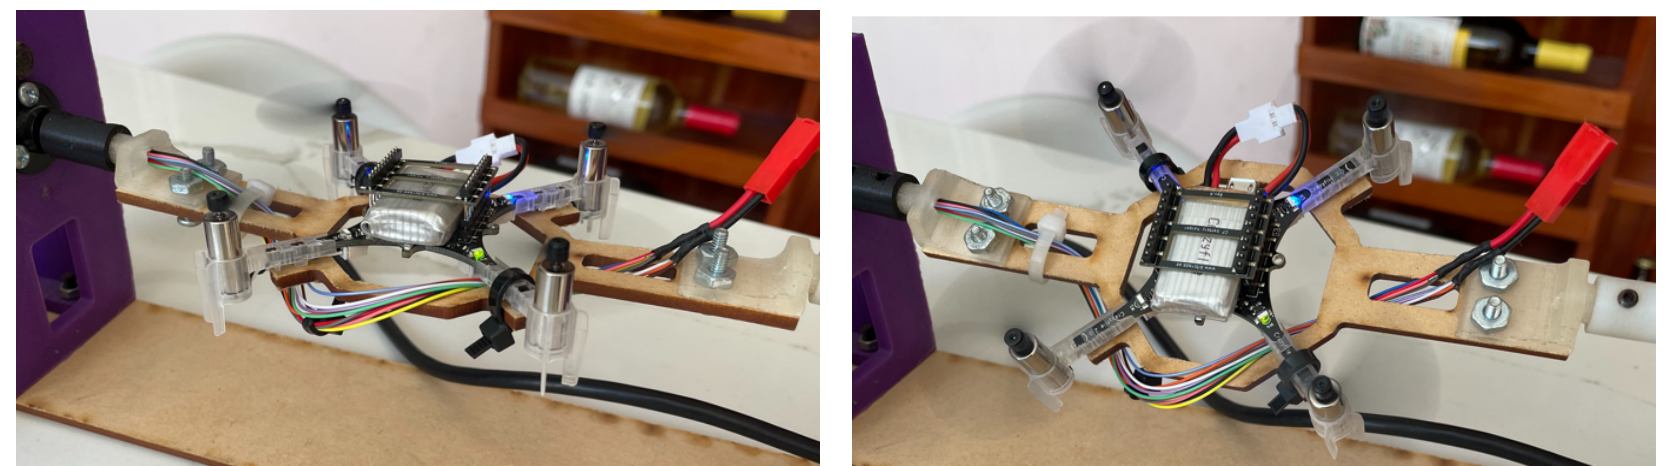
\includegraphics[width=0.75\textwidth]{Sanabria2022}
	\caption{Plataforma de pruebas de la investigación de Sanabria \cite{Sanabria2022_tesis}.}
	\label{fig:Sanabria2022}
\end{figure}

Como resultado de la investigación se crearon guías de laboratorio para los cursos de sistemas de control 1 y 2, con la limitante de que el dron únicamente podría utilizarse junto a la plataforma de pruebas.

\section{Ecosistema Robotat}
El ecosistema Robotat \ref{fig:Robotat} es un entrono tecnológico de investigación y experimentación ubicado en la Universidad del Valle de Guatemala \cite{Parafan2022_tesis}. Este ecosistema consiste de una plataforma sólida de aproximadamente $400\times 500$ cm, un sistema de captura de movimiento compuesto por seis cámaras OptiTrack y una red local Wi-Fi estblecida mediante el protocolo MQTT. La infraestructura permite la conexión y control de múltiples agentes simultáneamente, con una capacidad máxima de 11 agentes operando a una frecuencia de recepción y decodificación de datos superior a 10 Hz. 

\vspace{0.3cm} % Espacio antes de la imagen
\begin{figure}[htbp]
	\centering
	\includegraphics[width=0.75\textwidth]{Robotat}
	\caption{Ecosistema de pruebas Robotat \cite{Parafan2022_tesis}.}
	\label{fig:Robotat}
\end{figure}

\section{Incorporación de drones Crazyflie al ecosistema Robotat}
Denny Otzoy \cite{Otzoy2023_tesis} y José Gordillo \cite{Gordillo2023_tesis} se centraron en desarrollar la infraestructura y herramientas necesarias para utilizar el cuadricóptero dentro del ecosistema Robotat. Otzoy se enfocó en el desarrollo de herramientas para la integración con el sistema de captura de movimiento. Empleó una máquina física para la transmisión de datos, desarrolló la representación del dron como cuerpo rígido dentro del ecosistema y codificó las trayectorias en el formato adecuado. Por otro lado, Gordillo implementó un paquete de herramientas de \textit{software} para la ejecución de trayectorias de enjambre. Evaluó dos alternativas para el sistema de control y con base en un listado de ventajas y desventajas, descartó la opción de la librería Crazyswarm y en su lugar optó por implementar un sistema basado en una antena de comunicación WiFi. En ambos casos, a pesar de los esfuerzos, no se logró el control adecuado o seguimiento de trayectorias debido a limitantes en la metodología empleada para el sistema de control del dron. 

A raíz de las limitaciones encontradas, Julio Avila \cite{Avila2023_tesis} y Brandon Garrido \cite{Garrido2023_tesis} buscaron integrar la librería de control Crazyswarm 2 al ecosistema Robotat. El trabajo de Avila estuvo centrado principalmente en el desarrollo de un servidor para comunicación entre los drones, el sistema de captura de movimiento y Matlab, con el fin de enviar comandos para realizar trayectorias de drones individuales o de enjambre. Por su parte, Garrido se enfocó en el desarrollo de infraestructura para la experimentación y control de múltiples drones desde el sistema operativo ROS2 y dentro del ecosistema Robotat. Los resultados obtenidos en ambas investigaciones demostraron estabilidad y precisión en el control de los drones. 

\vspace{0.5cm} % Espacio antes de la imagen
\begin{figure}[htbp]
	\centering
	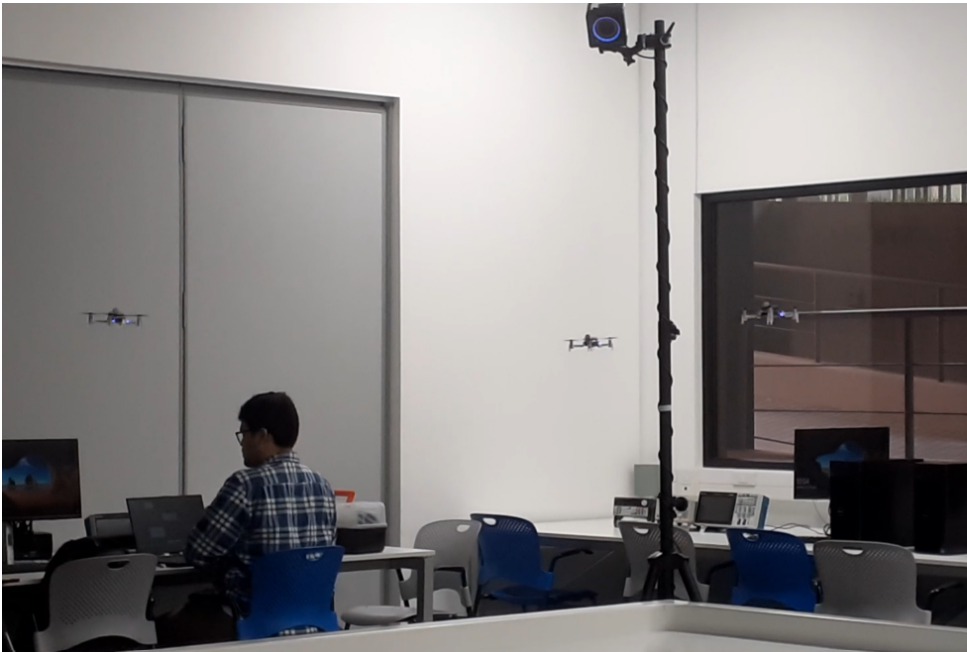
\includegraphics[width=0.75\textwidth]{Crazyswarm}
	\caption{Prueba de vuelo con 3 drones utilizando el \textit{software} Crazyswarm 2 \cite{Garrido2023_tesis}.}
	\label{fig:Crazyswarm}
\end{figure}
\vspace{0.4cm} % Espacio después de la imagen

Aunque el manejo de los drones mediante Crazyswarm demostró ser efectivo, requiere conocimientos de los sistemas operativos Linux y ROS2. Esta tarea vuelve complicado el proceso debido a la complejidad de dichas herramientas y la escasa documentación disponible de la librería Crazyswarm 2. Adicionalmente, la transición de Crazyflie a ROS2 es reciente, al igual que la librería Crazyswarm 2, lo que dificulta su implementación en laboratorios. 

Por otro lado, el uso individual de los drones Crazyflie plantea otro desafío, ya que, sin un medio para conocer su posición, los drones son vulnerables a colisiones debido a la fragilidad de su manipulación. Para abordar dicho desafío, una solución viable es complementar el funcionamiento de los drones con alguna de las placas de expansión de Bitcraze. Una de ellas es el Flow Deck, que ha demostrado ser altamente eficiente en proporcionar estabilidad al dron y con el cual se han logrado proyectos de investigación como vuelo autónomo y seguimiento de trayectorias.

\newpage
\section{Vuelo autónomo del dron Crazyflie 2.1 empleando la placa de posicionamiento Flow Deck}
En la Universidad Uppsala \cite{Chadehumbe2020_tesis} se realizó una investigación utilizando drones Crazyflie 2.1 con el objetivo de incorporar vuelo autónomo a través de trayectorias con obstáculos. Para ello se exploraron dos alternativas para el sistema de navegación del dron: un sistema de posicionamiento local mediante la herramienta LPS (\textit{Loco Positioning System}) y un sistema de navegación óptico mediante el dispositivo Flow Deck. Para la detección de obstáculos en las trayectorias se utilizó el sensor de detección Multiranger. 

Durante los experimentos realizados se observó que el sistema de navegación óptico superó al LPS en términos de estabilidad de vuelo y capacidad para completar las trayectorias. No se logró completar pruebas realizadas con el LPS como sistema de posicionamiento, siendo la razón principal el vuelo inestable causado por perturbaciones inusuales en el entorno de experimentación. Por otro lado, se completaron satisfactoriamente las pruebas al emplear el sistema de navegación óptico con el Flow Deck. Como recomendación, se sugirió realizar pruebas adicionales para mejorar la precisión del vuelo y considerar la posibilidad de utilizar múltiples sistemas de navegación en conjunto para obtener resultados más robustos.
    \fi  
\fi

% JUSTIFICACIÓN
% ------------------------------------------------------------------------------
\ifdefined\CAPjustificacion
	\newpage
	\chapter{Justificación}
	\ifdefined\parpordefecto
		\defaultparformat{f-justificacion}
	\else
		Los avances en investigación de ingeniería de control han sido significativamente influenciados por el uso de drones, que se han convertido en herramientas indispensables debido a su alta capacidad para implementar algoritmos de control. Su versatilidad y facilidad de adaptación hacen de los drones un recurso valioso para la enseñanza de cursos relacionados con ingeniería de control y robótica. 

En la Universidad del Valle de Guatemala, se han desarrollado distintos proyectos de investigación que han aprovechado las capacidades de los drones Crazyflie. Estos proyectos han explorado distintas aplicaciones, desde su uso en plataformas de pruebas hasta la formación de enjambres de drones en entornos controlados. 

Recientemente, se ha desarrollado un conjunto de herramientas que, si bien demostraron ser efectivas, resultan complicadas de utilizar debido a su alta curva de aprendizaje y escasa documentación. En particular, la herramienta Crazyswarm 2 en ROS2 ha demostrado ser efectiva pero difícil de manejar debido a los requerimientos de conocimientos avanzados en Linux y ROS2, así como la falta de documentación disponible. Por ello, surge la necesidad de simplificar las herramientas para facilitar el uso práctico y seguro de los drones.

El propósito de este trabajo de graduación se centra en la oportunidad de ampliar el uso de los drones Crazyflie en la Universidad del Valle de Guatemala, permitiendo su uso independiente y seguro mediante la integración de la placa de expansión para posicionamiento Flow Deck. De esta manera, los drones podrán ser utilizados de forma sencilla en prácticas de laboratorio en cursos de ingeniería electrónica y mecatrónica, como sistemas de control 1 y 2.  

	\fi
\fi

% OBJETIVOS
% ------------------------------------------------------------------------------
\ifdefined\CAPobjetivos
	\newpage
	\chapter{Objetivos}
	\ifdefined\parpordefecto
		\defaultparformat{g-objetivos}
	\else
		\subsection*{Objetivo general}
Desarrollar herramientas de software para controlar de manera individual y segura el cuadricóptero Crazyflie 2.1 utilizando la placa de expansión de posicionamiento con odometría visual Flow Deck.

\subsection*{Objetivos específicos}
\begin{itemize}
	\item Realizar la integración, pruebas y validación de la placa de expansión Flow Deck en el dron Crazyflie 2.1 sobre la mesa de pruebas del ecosistema Robotat.  
	\item Desarrollar herramientas de software que permitan simular, controlar y monitorear a los drones Crazyflie 2.1 de forma independiente y segura.
	\item Desarrollar un conjunto de experimentos que permitan estudiar temas de control de orientación y posición del dron Crazyflie 2.1 en la mesa de trabajo del ecosistema Robotat y que puedan emplearse dentro de los cursos de Sistemas de Control y Robótica. 
\end{itemize}

	\fi
\fi

% ALCANCE
% ------------------------------------------------------------------------------
\ifdefined\CAPalcance
	\newpage
	\chapter{Alcance}
	\ifdefined\parpordefecto
    	\defaultparformat{h-alcance}
    \else
    	Este proyecto tiene como alcance la integración y validación de la placa de expansión Flow Deck en los drones Crazyflie 2.1 de la Universidad del Valle de Guatemala, utilizando las herramientas y librerías otorgadas por el fabricante. Además, se busca desarrollar herramientas de \textit{software} simplificadas que permitan el control básico de los drones y faciliten su uso dentro de un entorno educativo de laboratorio.

Se propone también la creación de dos guías de laboratorio para cursos impartidos en la Universidad del Valle de Guatemala. La primera para el curso de Sistemas de Control 1, enfocada en la modificación del controlador PID de posición para el control de altura del dron. La segunda para el curso de Robótica 1, en la que se desarrollarán experimentos de seguimiento de trayectorias con obstáculos. Finalmente, se elaborará un manual de usuario para el Crazyflie 2.1 con la placa Flow Deck integrada, para que los usuarios puedan familizarizarse con su configuración y manejo. 
    \fi 
\fi

% MARCO TEÓRICO
% ------------------------------------------------------------------------------
\ifdefined\CAPmarcoteorico
	\newpage
	\chapter{Marco teórico}
	\ifdefined\parpordefecto
		\defaultparformat{i-marco_teorico}
	\else
		Para alcanzar los objetivos planteados, es necesario abordar una serie de temas claves que proporcionarán contexto y comprensión técnica necesarios para desarrollar el proyecto. 

\subsection*{Crazyflie 2.1 }
Los drones Crazyflie son plataformas de desarrollo aéreo de código abierto desarrollados por Bitcraze. Están diseñados principalmente para investigación, desarrollo y educación en ingeniería de control y robótica. Como se observa en la Figura \ref{fig:Crazyflie}, tienen un tamaño reducido, pero están equipados con una variedad de sensores que lo vuelven ideal para explorar algoritmos de control y otras aplicaciones. 
\begin{figure}[htbp]
	\centering
	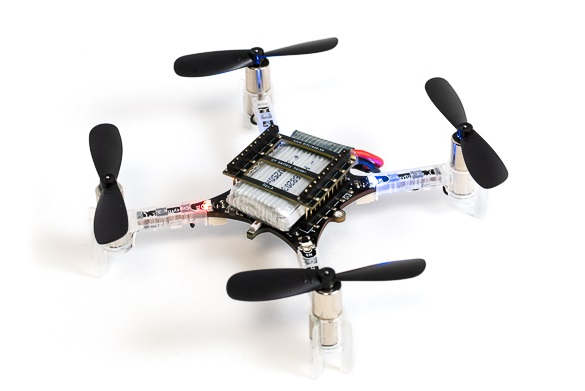
\includegraphics[width=0.45\textwidth]{Crazyflie}
	\caption{Dron Crazyflie 2.1 \cite{Crazyflie}.}
	\label{fig:Crazyflie}
\end{figure}
\\El Crazyflie 2.1 es un mini dron que pesa aproximadamente 27 gramos y tiene dimensiones generales de 92mm x 92mm x 29mm. Su control se realiza mediante Bluetooth o radiofrecuencia, lo que le permite ser controlado desde dispositivos móviles, así como desde sistemas operativos Windows, Mac OSX y Linux utilizando Crazyradio o Crazyradio PA. En cuanto a sus características eléctricas, el Crazyflie 2.1 dispone de una batería de litio-polímero (Li-Po) con modos desde 100 mA hasta 980 mA, que alimenta motores, microcontroladores y demás componentes. Utiliza un microcontrolador STM32F405 para el control de vuelo y un microcontrolador nRF51 para la comunicación inalámbrica. Está equipado con un acelerómetro/giroscopio de 3 ejes BMI088 y un sensor de presión de alta precisión BMP388, pero también permite la integración de otras placas de expansión para ampliar sus capacidades, con la restricción de que soporta una carga adicional de hasta 15 gramos que puede afectar el tiempo de vuelo debido al aumento de demanda de energía \cite{Crazyflie}. 

\subsection*{Sistema de coordenadas de drones Crazyflie}
Los drones Crazyflie, al igual que la mayoría de los drones, utilizan la convención de sistema de coordenadas tridimensional ENU (East North Up) para determinar su posición y orientación en el espacio. Como se observa en la Figura \ref{fig:Sistema_Crazyflie}, el dron tiene tres ejes principales de referencia: el eje X es horizontal y apunta hacia adelante, el eje Y es horizontal y apunta hacia la derecha y el eje Z es vertical y apunta hacia arriba. 

Por otro lado, la orientación del dron se describe en términos de ángulos de inclinación respecto a los ejes de referencia. El ángulo de balanceo (roll) se refiere a la inclinación del dron hacia los lados en torno al eje X, el ángulo de cabeceo (pitch) se refiere a la inclinación hacia adelante o hacia atrás en torno al eje Y, y el ángulo de guiñada (yaw) se refiere a la rotación del dron en torno al eje Z. Según la documentación oficial de Bitcraze, estos ángulos siguen las siguientes reglas de rotación: roll y yaw rotan en sentido horario alrededor del eje al mirar desde el origen, mientras que pitch rota en sentido antihorario alrededor del eje al mirar desde el origen \cite{Sistema_Crazyflie}.

\begin{figure}[htbp]
	\centering
	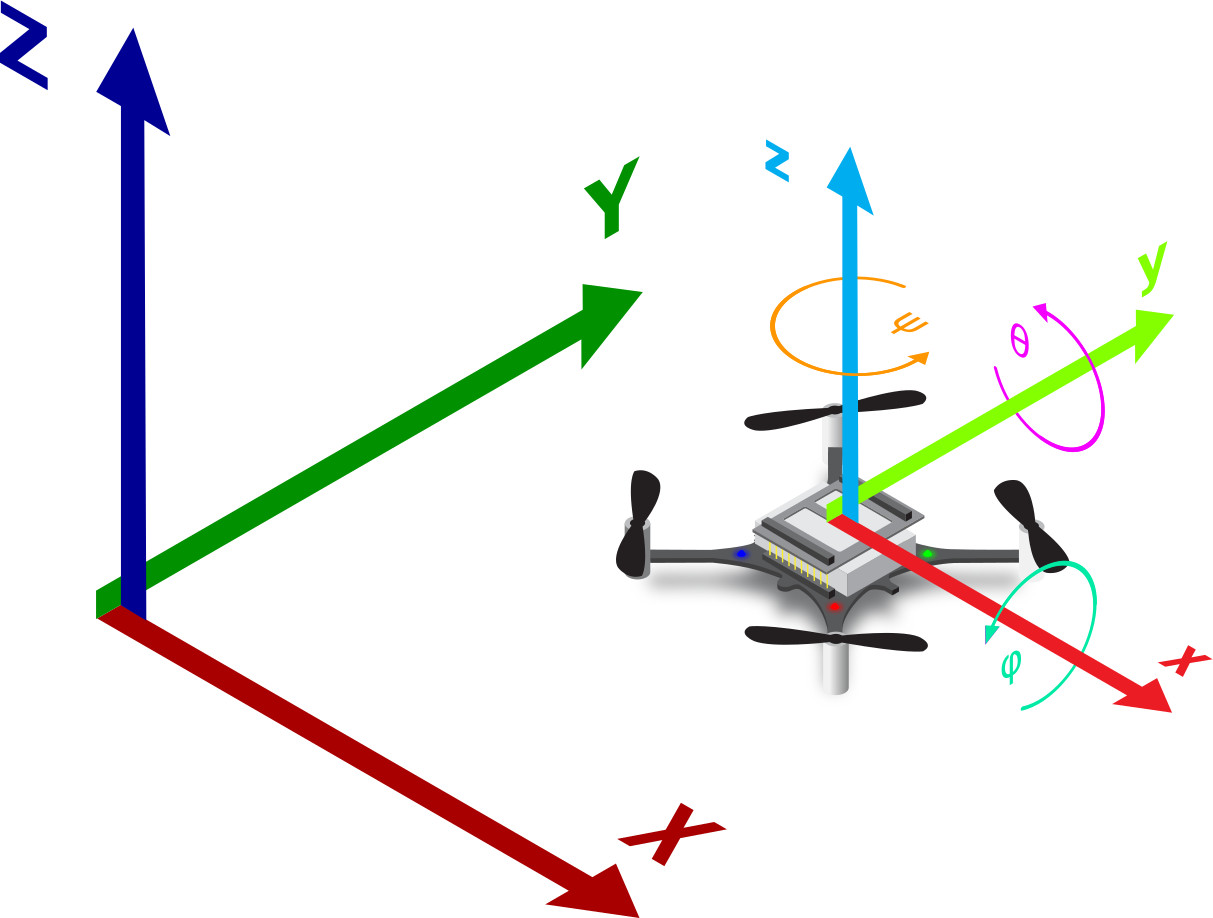
\includegraphics[width=0.6\textwidth]{Sistema_Crazyflie}
	\caption{Sistema de coordenadas de Crazyflie 2.1 \cite{Sistema_Crazyflie}.}
	\label{fig:Sistema_Crazyflie}
\end{figure}

\subsection*{Comunicación inalámbrica de drones Crazyflie}
Los drones Crazyflie establecen una comunicación inalámbrica por medio del dispositivo Crazyradio, mostrado en la Figura \ref{fig:Crazyradio}. Esta comunicación se basa en un enlace de radiofrecuencia bidireccional que permite enviar comandos de control al dron y recibir datos en tiempo real sobre su posición, orientación y otros parámetros relevantes.   
\begin{figure}[htbp]
	\centering
	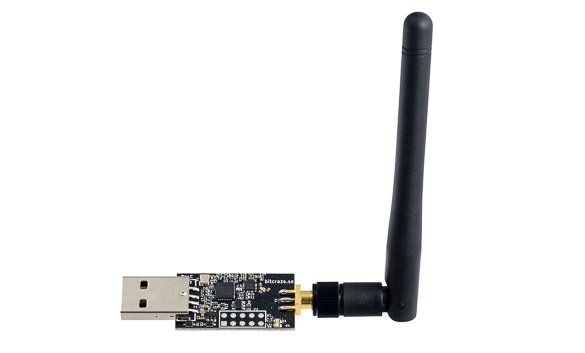
\includegraphics[width=0.4\textwidth]{Crazyradio}
	\caption{Dispositivo de comunicación inalámbrica Crazyradio \cite{Crazyradio}.}
	\label{fig:Crazyradio}
\end{figure}
\\ El Crazyradio es un transceptor de radio USB de código abierto, baja latencia y largo alcance. Funciona en la banda de 2.4 GHz con un rango de transmisión de hasta 1 km (en condiciones ideales) gracias a su amplificador de radio de 20 dBm. Está basado en el microcontrolador nRF24LU1 de Nordic Semiconductor y se comunica por medio del protocolo “Enhanced ShockBurst” compatible con los microcontroladores nRF24L01p, nRF51 y nRF52. En una capa de nivel más alto, utiliza el protocolo de paquetes CRTP para comunicarse con el Crazyflie y poder actualizar el firmware, enviar comandos y recibir información de los drones. Dependiendo del sistema operativo, es necesario instalar controladores o realizar configuraciones específicas \cite{Crazyradio}.

\subsection*{Flow Deck}
El Flow Deck es una placa de expansión para el dron Crazyflie y que le otorga la capacidad de comprender su movimiento en cualquier dirección. Utiliza un medición de distancias VL53L1x para determinar su altura junto a un sensor de flujo óptico PMW3901 que mide movimientos horizontales sobre la superficie por medio de odometría visual.  La placa de expansión Flow Deck, mostrada en la Figura \ref{fig:FlowDeck}, tiene un peso aproximado de 1,6 gramos y dimensiones generales de 21mm x 28mm x 4mm. Para integrarlo se requiere actualizar el firmware del Crazyflie a su última versión y montarlo en la parte inferior del dron. \cite{FlowDeck}. 
\begin{figure}[htbp]
	\centering
	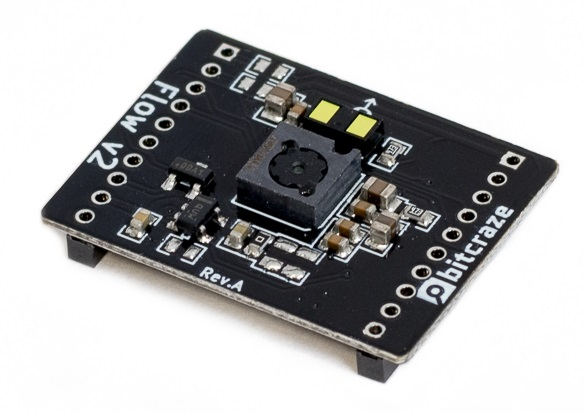
\includegraphics[width=0.35\textwidth]{FlowDeck}
	\caption{Placa de expansión Flow Deck v2 \cite{FlowDeck}.}
	\label{fig:FlowDeck}
\end{figure}
\subsection*{Odometría visual}
La odometría visual es un proceso mediante el cual se utiliza información extraída de imágenes para estimar el movimiento, en este caso relacionado con un vehículo o robot. En esta técnica de estimación de posición se emplea una secuencia de imágenes para calcular la trayectoria de rasgos visuales distintivos en las imágenes y el análisis de cómo estos cambian entre imágenes consecutivas. Los sistemas de odometría visual son capaces de generar un mapa tridimensional del entorno y un registro de la trayectoria para determinar la localización del agente. En esencia, la odometría visual se basa en la geometría de las imágenes capturadas por cámaras, utilizando algoritmos para minimizar la proyección repetitiva de puntos tridimensionales a partir de las características visuales coincidentes entre imágenes \cite{Persson2022_book}. 
\begin{figure}[htbp]
	\centering
	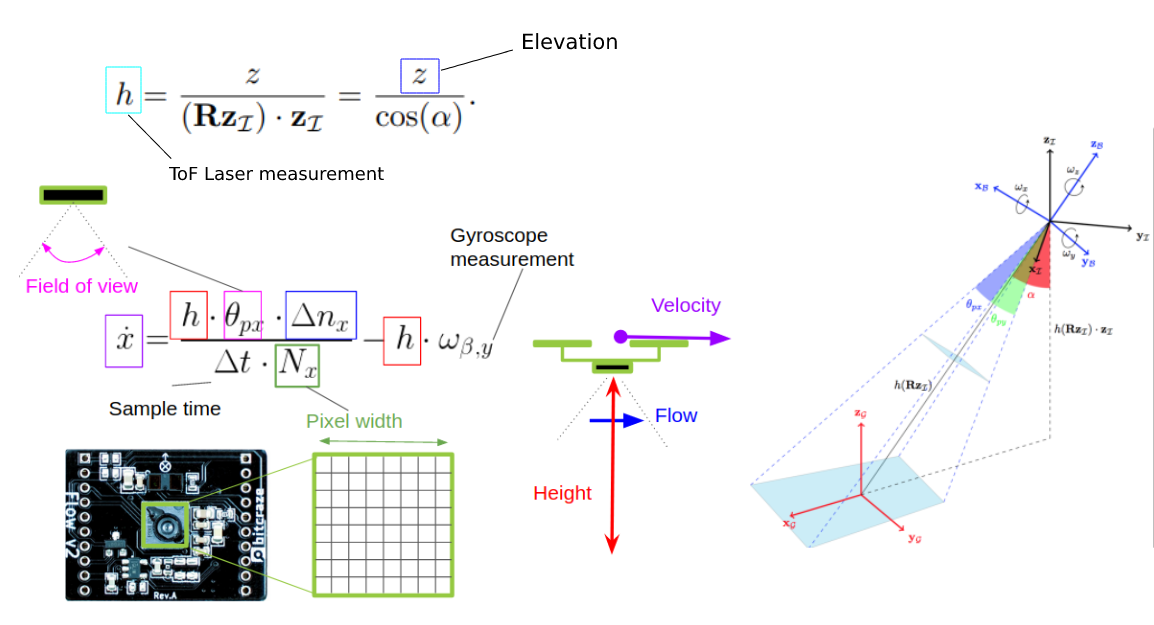
\includegraphics[width=0.7\textwidth]{Funcionamiento_FlowDeck}
	\caption{Gráfico de funcionamiento de Flow Deck \cite{Funcionamiento_FlowDeck}.}
	\label{fig:Funcionamiento_FlowDeck}
\end{figure}
\\Como se mencionó con anterioridad y justo como se evidencia en la Figura \ref{fig:Funcionamiento_FlowDeck}, el Flow Deck utiliza odometría visual para obtener las mediciones de posición en el plano horizontal. Esta información se combina con las mediciones del sensor de distancia para determinar la posición del Crazyflie en relación con su entorno. \cite{Funcionamiento_FlowDeck}.

 \subsection*{Sensor de flujo óptico PMW3901}
El PMW3901 es un sensor de flujo óptico desarrollado por Pixart Imaging, ampliamente utilizado en aplicaciones de robótica para medir movimiento. Resulta de particular interés debido a que forma parte de la placa de expansión Flow Deck de Bitcraze y es el responsable de darle sentido de posición bidimensional (en los ejes X-Y) a los drones Crazyflie. Dentro de sus detalles técnicos, dispone un microcontrolador de bajo consumo que determina internamente el flujo óptico con algoritmos de odometría visual, proporcionando posición con base en diferencias en pixeles entre fotogramas. Opera con un voltaje que varía entre 1.8 y 2.1V. Se comunica por medio de una interfaz SPI de 4 hilos que opera a 2 MHz, transmitiendo datos de movimiento almacenados en registros de 16 bits. Tiene un rango de operación desde 80 mm hasta el infinito y cuenta con una tasa de fotogramas de 121 FPS, detectando movimientos de hasta 7.4 radianes por segundo. Finalmente, está encapsulado en un paquete chip-on-board de 28 pines, lo que permite su integración en distintas aplicaciones \cite{PMW3901_datasheet}.

\subsection*{Sensor de medición de distancias VL53L1x}
El VL53L1x es un sensor de medición de distancias desarrollado por STM electronics. La placa de expansión Flow Deck tiene integrado este sensor para proporcionar sentido de altura de vuelo (eje Z) a los drones Crazyflie. En cuanto a sus especificaciones técnicas, el VL53L1x está basado en la tecnología de tiempo de vuelo (Time-of-Flight, ToF) que permite medir el tiempo que tarde un pulso de luz en reflejarse desde un objeto y volver al sensor, proporcionando una medida precisa de la distancia del objeto. El sensor funciona emitiendo un láser invisible de 940 nm y utiliza una matriz de recepción SPAD (diodo de avalancha de fotón único) para detectar la luz reflejada, ofreciendo un campo de visión típico de 27 grados. Incluye un microcontrolador de bajo consumo que permite una medición de distancia de hasta 4 metros con una frecuencia de hasta 50 Hz y se comunica por medio de una interfaz I2C que soporta velocidades de hasta 400 kHz \cite{VL53L1x_datasheet}.

\subsection*{Librería en Python para Crazyflie}
Existe una librería en Python desarrollada por el grupo Bitcraze cuya función es simplificar el uso y control de los drones Crazyflie. Esta librería disponde de funciones de alto nivel que facilitan la conexión, registro de datos, envío de comandos y manipulación de parámteros del dron. Está diseñada para ser utilizada con los drones Crazyflie por medio del dispositivo Crazyradio, admitiendo enlaces de comunicación mediante diferentes interfases tales como radio, USB, serial, entre otras. Dentro de las funciones de alto nivel que presenta, están algunas para envío de comandos de control de actitud y posición, así como otras para configuración de registros y monitoreo de variables del firmware en tiempo real \cite{Crazyflie_Python}. 

\subsection*{Protocolo de comunicación CRTP}
CRTP es el protocolo de empaquetamiento de datos utilizado para comunicarse con los drones Crazyflie. Este protocolo estructura los paquetes de información para dirigirlos a funcionalidades específicas del dron como el registro de datos, control de movimiento y parámetros de configuración \cite{Crazyflie_CRTP}. 

\subsubsection*{Pila de comunicación}
La comunicación con Crazyflie se implementa como una pila de capas independientes. En la base se encuentra el medio físico (radio o USB), seguido por el enlace que garantiza la transmisión segura y ordenada de paquetes. Encima de esto está CRTP que maneja información de puerto y canal para dirigir los paquetes de datos a los distintos subsistemas del Crazyflie. Por último, los subsistemas implementan las funcionalidades del dron, controladas a través de CRTP.

\subsubsection*{Implementación de enlaces}
Existen dos implementaciones de enlace activamente soportadas para Crazyflie: el enlace de radio, que utiliza radios compatibles con nRF24, y el enlace USB, que se conecta directamente al puerto USB del Crazyflie. Cada uno de estos enlaces asegura la transmisión ordenada y segura de paquetes entre el controlador y el dron.

\subsubsection*{Ordenación de paquetes y soporte en tiempo real}
CRTP (Crazy RealTime Protocol) prioriza los paquetes para facilitar el control en tiempo real del Crazyflie. El enlace garantiza el orden estricto de los paquetes dentro de un mismo puerto, aunque los paquetes de diferentes puertos pueden enviarse fuera de orden. La priorización se logra asignando mayor prioridad a los números de puerto más bajos, permitiendo la transmisión simultánea de datos en tiempo real y la carga de trayectorias.

\subsubsection*{Metadatos del paquete CRTP}
Cada paquete CRTP incluye un número de puerto, un número de canal y una carga útil. Los puertos oscilan entre 0 y 15 y los canales entre 0 y 3, con la carga útil limitada a 31 bytes. Estos metadatos permiten dirigir los paquetes a los subsistemas correctos y las funcionalidades específicas dentro del Crazyflie.

\subsubsection*{Paquetes especiales}
El paquete 15:3 es un caso especial denominado null packet, que es ignorado por el Crazyflie y las bibliotecas CRTP. Los null packets se usan para solicitar datos descendentes cuando no hay datos para enviar. También se utilizan para comunicar paquetes fuera del flujo de datos principal, como los paquetes de bootloader, interpretados por el chip de radio nRF51 del Crazyflie.

\subsubsection*{Asignación de puertos}
Los puertos CRTP se asignan a distintos subsistemas en el Crazyflie, permitiendo la comunicación bidireccional entre un subsistema específico y su manejador en tierra. Por ejemplo, el puerto 0 se utiliza para leer el texto de la consola, el puerto 2 para obtener y establecer parámetros, y el puerto 3 para enviar puntos de control de movimiento.

\subsubsection*{Procedimiento de conexión}
Generalmente, CRTP es sin conexión y la mayoría de los subsistemas del Crazyflie intentan ser sin estado. Sin embargo, algunos enlaces y subsistemas mantienen estados específicos, como el enlace USB que necesita ser habilitado mediante un paquete de control USB, y el enlace de radio que utiliza contadores de paquetes para evitar pérdidas y garantizar el orden. La conexión típica incluye inicializar el enlace y los subsistemas soportados, asegurando la transmisión de datos correcta y segura.
	\fi
\fi

% CAPÍTULOS
% ------------------------------------------------------------------------------
\newpage
\ifdefined\parpordefecto
	\defaultparformat{j-capitulos}
\else
	% ------------------------------------------------------------------------------
% CAPÍTULO 7 -------------------------------------------------------------------
% ------------------------------------------------------------------------------
\chapter{Integración y validación de la placa de expansión Flow Deck}
En este capítulo se presenta una explicación detallada del procedimiento realizado para lograr la integración exitosa de la placa de expansión Flow Deck en el dron Crazyflie 2.1. Para realizar esta tarea, se utilizó un ordenador con sistema operativo Windows 11 y \textit{software} de código abierto proporcionado por el grupo Bitcraze. También, se describen los experimentos de vuelo reaizados con y sin la placa de expansión Flow Deck y se proporcionan observaciones importantes, relacionadas con el entorno de experimentación, para que la placa funcione correctamente.

\section{Validación de funcionamiento de Crazyflie}
Previo a la instalación de la placa de expansión, fue necesario realizar una verificación del ensamble y ajustes de configuración con el fin de garantizar el funcionamiento adecuado del dron Crazyflie 2.1 para los fines del proyecto.

\subsection{Ensamble de Crazyflie}
Respecto al ensamble del dron, se consultó el tutorial de armado y pruebas de vuelo disponible en la página oficial de Bitcraze \cite{Crazyflie_tutorial_ensamble}. Se examinó que cada parte del dron estuviera correctamente instalada según la información en la página. El resultado obtenido se observa en la Figura \ref{fig:Crazyflie_ensamble} donde se muestra al dron correctamente ensamblado. 

\begin{figure}[htbp]
	\centering
	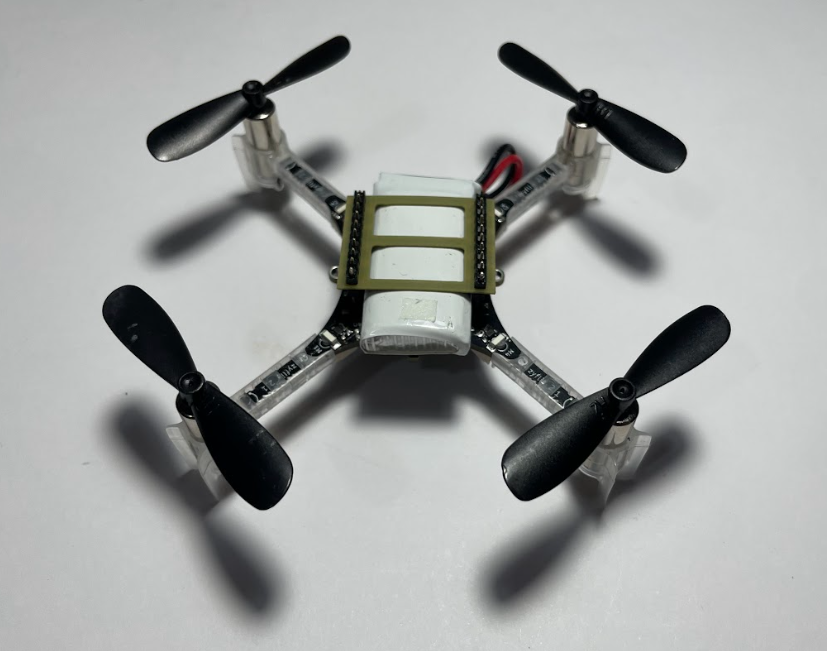
\includegraphics[width=0.4\textwidth]{Crazyflie_ensamblado}
	\caption{Ensamble correcto de dron Crazyflie 2.1.}
	\label{fig:Crazyflie_ensamble}
\end{figure}

Luego de examinar y validar el ensamble, se ejecutó la secuencia de autoprueba presionando el botón de encendido. Esta secuencia preparó al dron para volar, verificando que el \textit{hardware} se encontrara en buen estado y calibró los sensores con valores base. Para ejecutar la prueba, se colocó al dron en una superifice nivelada y se mantuvo absolutamente quieto.

La ejecución de la autoprueba indicó que el estado del dron se encontraba a la perfección y listo para volar. Esto se determinó con la siguiente lista de resultados que se interpretan con la modalidad de encendido de los LED presentes en el dron:
\begin{itemize}
	\item \textbf{Encendido y listo para volar:} LED azules permanecen encendidos y el LED delantero derecho parpadea en rojo dos veces por segundo.
	\item \textbf{Encendido pero con sensores descalibrados:} LED acules permanecen encendidos y el LED delantero derecho parapadea en rojo cada dos segundos.
	\item \textbf{Crazyradio conectada:} LED delantero izquierdo parpadea en rojo y/o verde.
	\item \textbf{Batería baja:} LED delantero derecho permanece completamente encendido en rojo.
	\item \textbf{Carga:} LED azul izquierdo parpadea mientras que el LED azul derecho está encendido.
	\item \textbf{Modo cargador de arranque:} LED azules parpadean una vez por segundo.
	\item \textbf{Error de autoprueba:} LED delantero derecho parpadea repetidamente en rojo con una pausa larga entre parpadeos.
\end{itemize}

\begin{figure}[htbp]
	\centering
	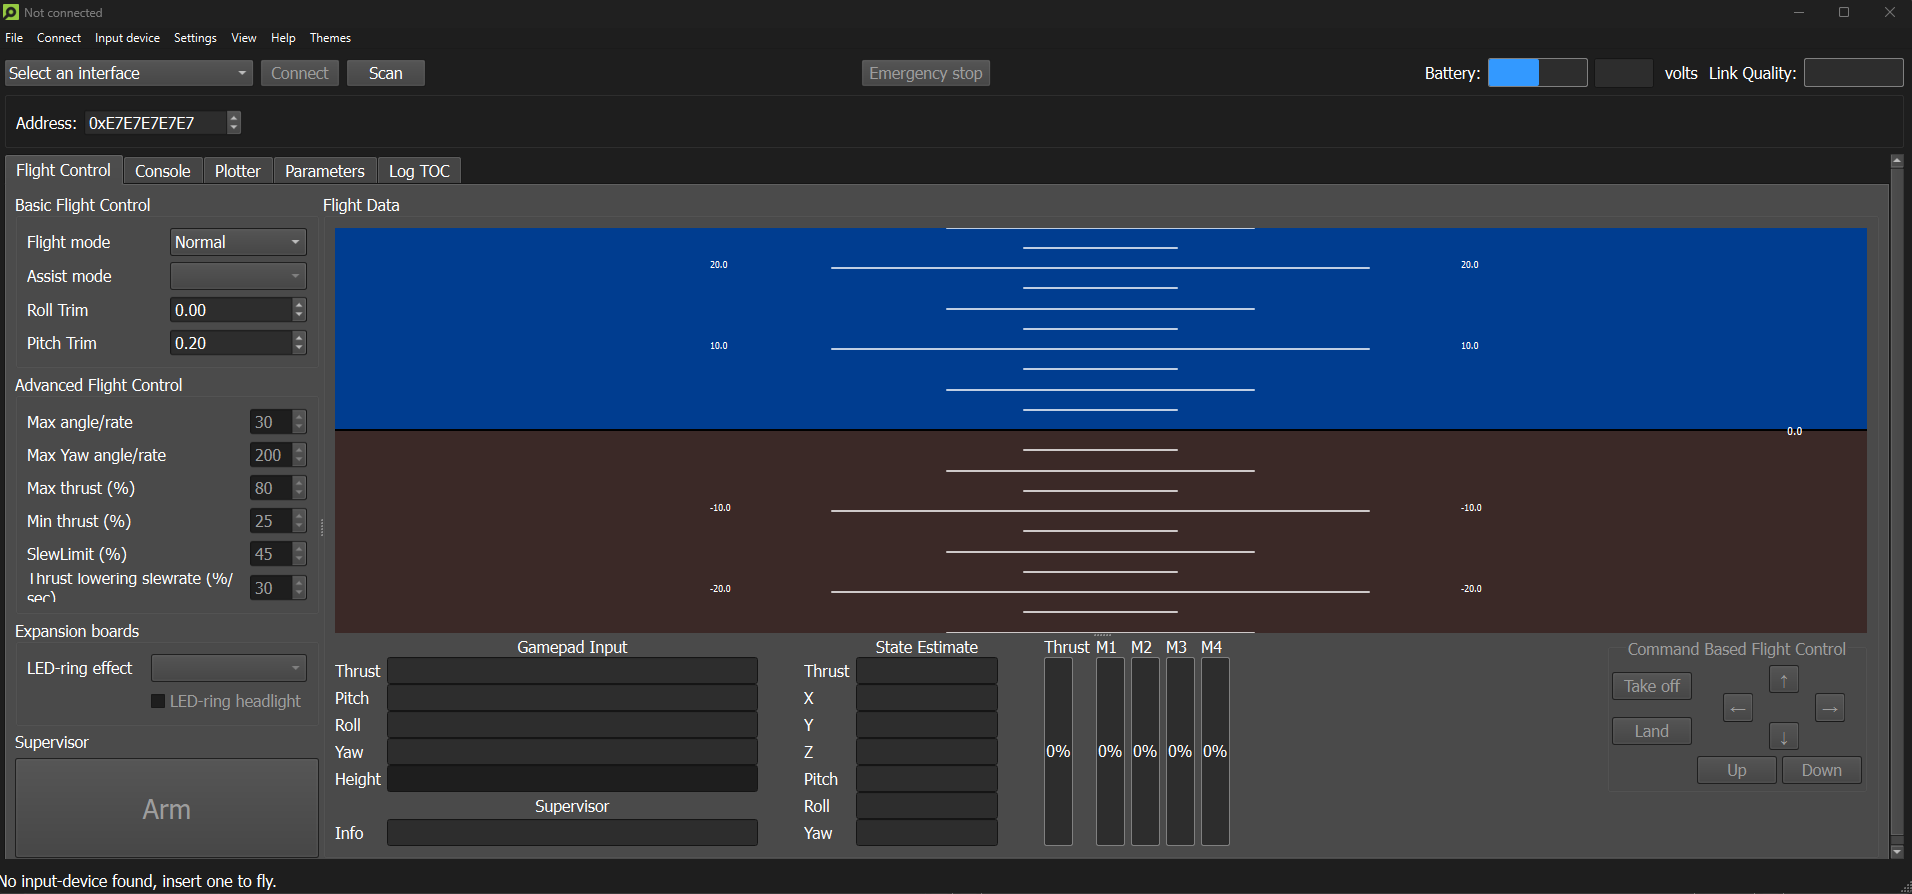
\includegraphics[width=0.85\textwidth]{Crazyclient}
	\caption{Interfaz de control de vuelo del \textit{software} Crazyclient.}
	\label{fig:Crazyclient}
\end{figure} 

\subsection{Software Crazyclient y actualización de firmware de Crazyflie}
Tras verificar que el dron iniciara correctamente, se instaló el \textit{software} de código abierto Crazyclient del grupo Bitcraze según el manual de instalación provisto en su página oficial \cite{Crazyflie_installation_Cfclient}. Se instaló la versión para Windows 10/11. Este programa dispone de diversas herramientas para el control, calibración, visualización de datos en tiempo real y configuración de parámetros del dron Crazyflie. Además, como se observa en la Figura \ref{fig:Crazyclient}, también dispone de una interfaz gráfica de usuario que facilita la interacción con el dron.

Una vez se ha instalado correctamente el programa Crazyclient, lo primero que se realizó fue la actualización de \textit{firmware} siguiendo las instrucciones en la página oficial \cite{Crazyflie_6}. Este paso es fundamental para que el dron Crazyflie sea capaz de reconocer a la placa de expansión Flow Deck. Es necesario que tenga instalada la versión más reciente disponible. para garantizar un rendimiento eficiente del \textit{hardware}.

\begin{figure}[htbp]
	\centering
	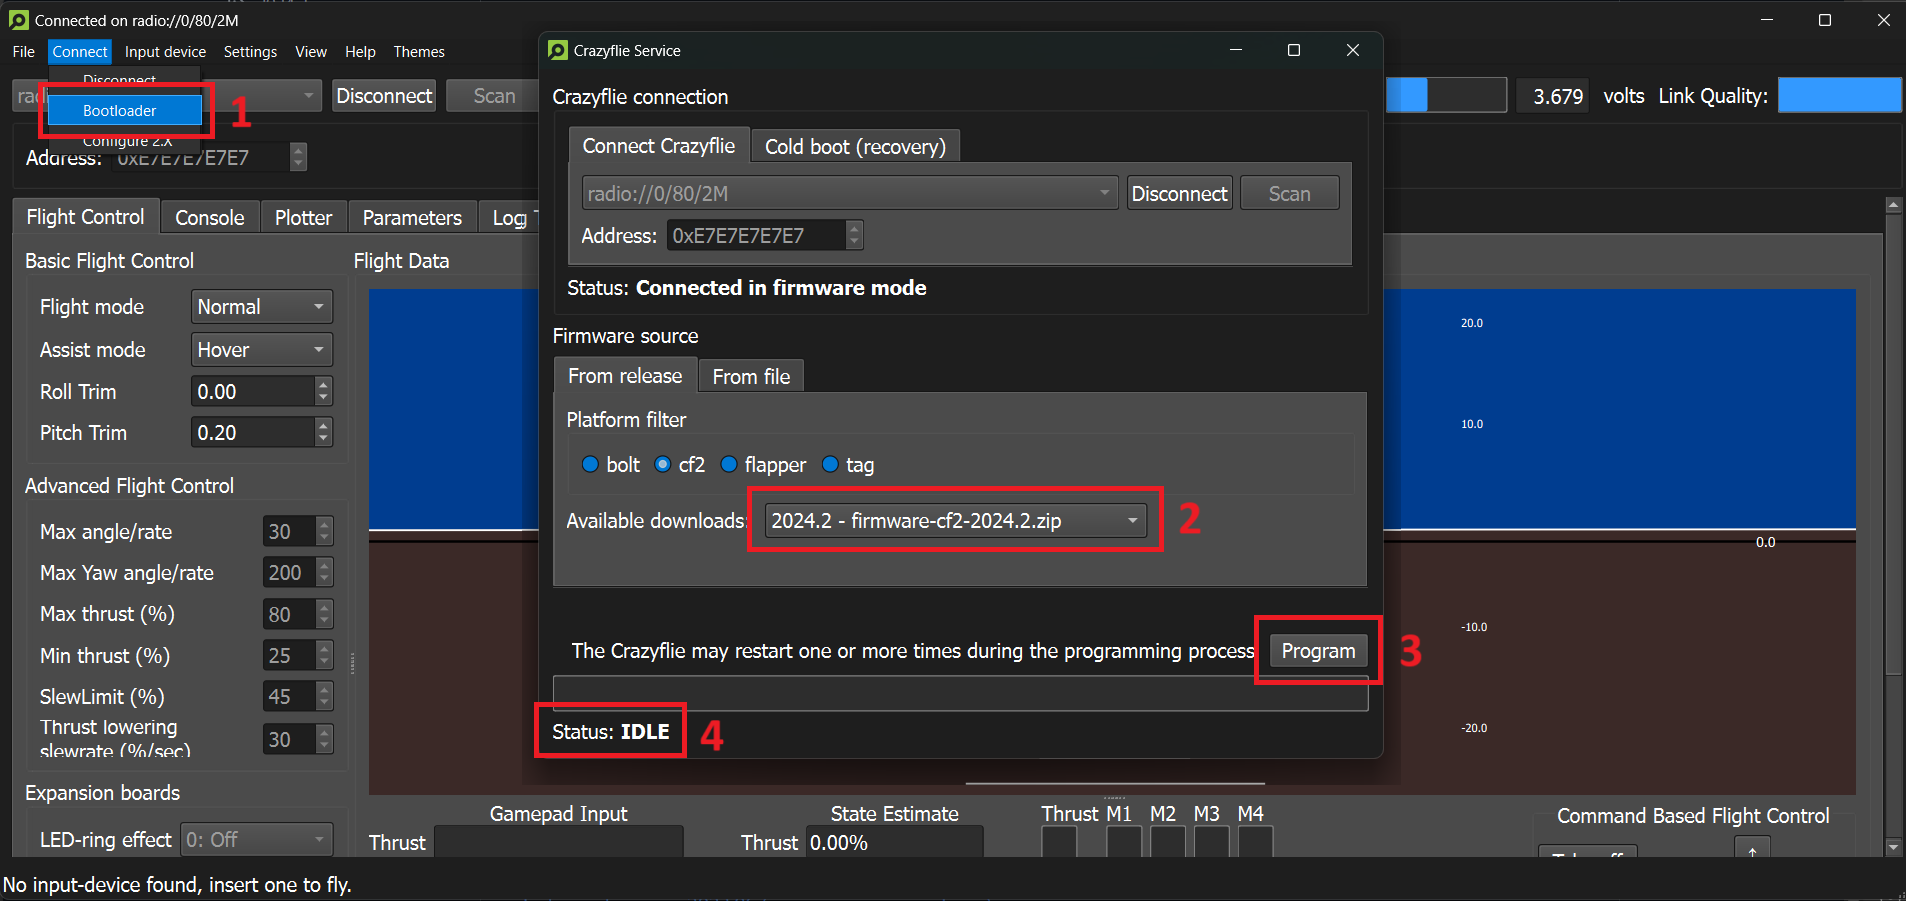
\includegraphics[width=0.85\textwidth]{Actualizacion_firmware}
	\caption{Actualización de \textit{firmware} con el programa Crazyclient.}
	\label{fig:Actualizacion_firmware}
\end{figure} 

Previo a la actualización de \textit{firmware}, fue necesario instalar los controladores USB del dispositivo Crazyradio utilizando la guía de instalación del fabricante \cite{Crazyflie_USB_driver}. Posteriormente, se empleó el Crazyradio para establecer la conexión con el Crazyflie. Una vez conectado, se siguió la serie de pasos mostrados en la Figura \ref{fig:Actualizacion_firmware}. Cabe mencionar que el último paso tan solo consiste en esperar a que termine el proceso y que el estado del dron sea IDLE. 

\subsection{Configuración de parámetros}
Como siguiente paso se habilitó la vista de parámetros del Cfclient para ajustar a los parámetros del dron con el fin de asegurar el comportamiento esperado.

\begin{itemize}
	\item \textbf{stabilizer.controller:} se colocó con un valor de 1 para utilizar el controlador PID.
	\item \textbf{stabilizer.estimator:} se colocó un valor de 2 para utilizar el estimador extendido de Kalman.
	\item \textbf{commander.enHighLevel:} se colocó un valor de 1 para permitir el envío de comandos de forma remota al dron.
\end{itemize}

\subsection{Prueba de hélices y motores}
Manteniendo la conexión del dron con el cliente, se utilizó la vista de consola para realizar una prueba de hélices y motores. Para ello, se colocó al Crazyflie sobre una superifcie plana y dura y luego se seleccionó la opción ``\textit{Propeller test}'' para realizar una prueba de vibración en motores y hélices (Figura \ref{fig:Propeller_test}). El dron accionó levemente los motores, de forma secuencial, para determinar el estado de estos y sus hélices. Para los motores que presentaron vibraciones por encima del umbral permitido se emitió un pitido y se imprimió la advertencia en consola.

\begin{figure}[htbp]
	\centering
	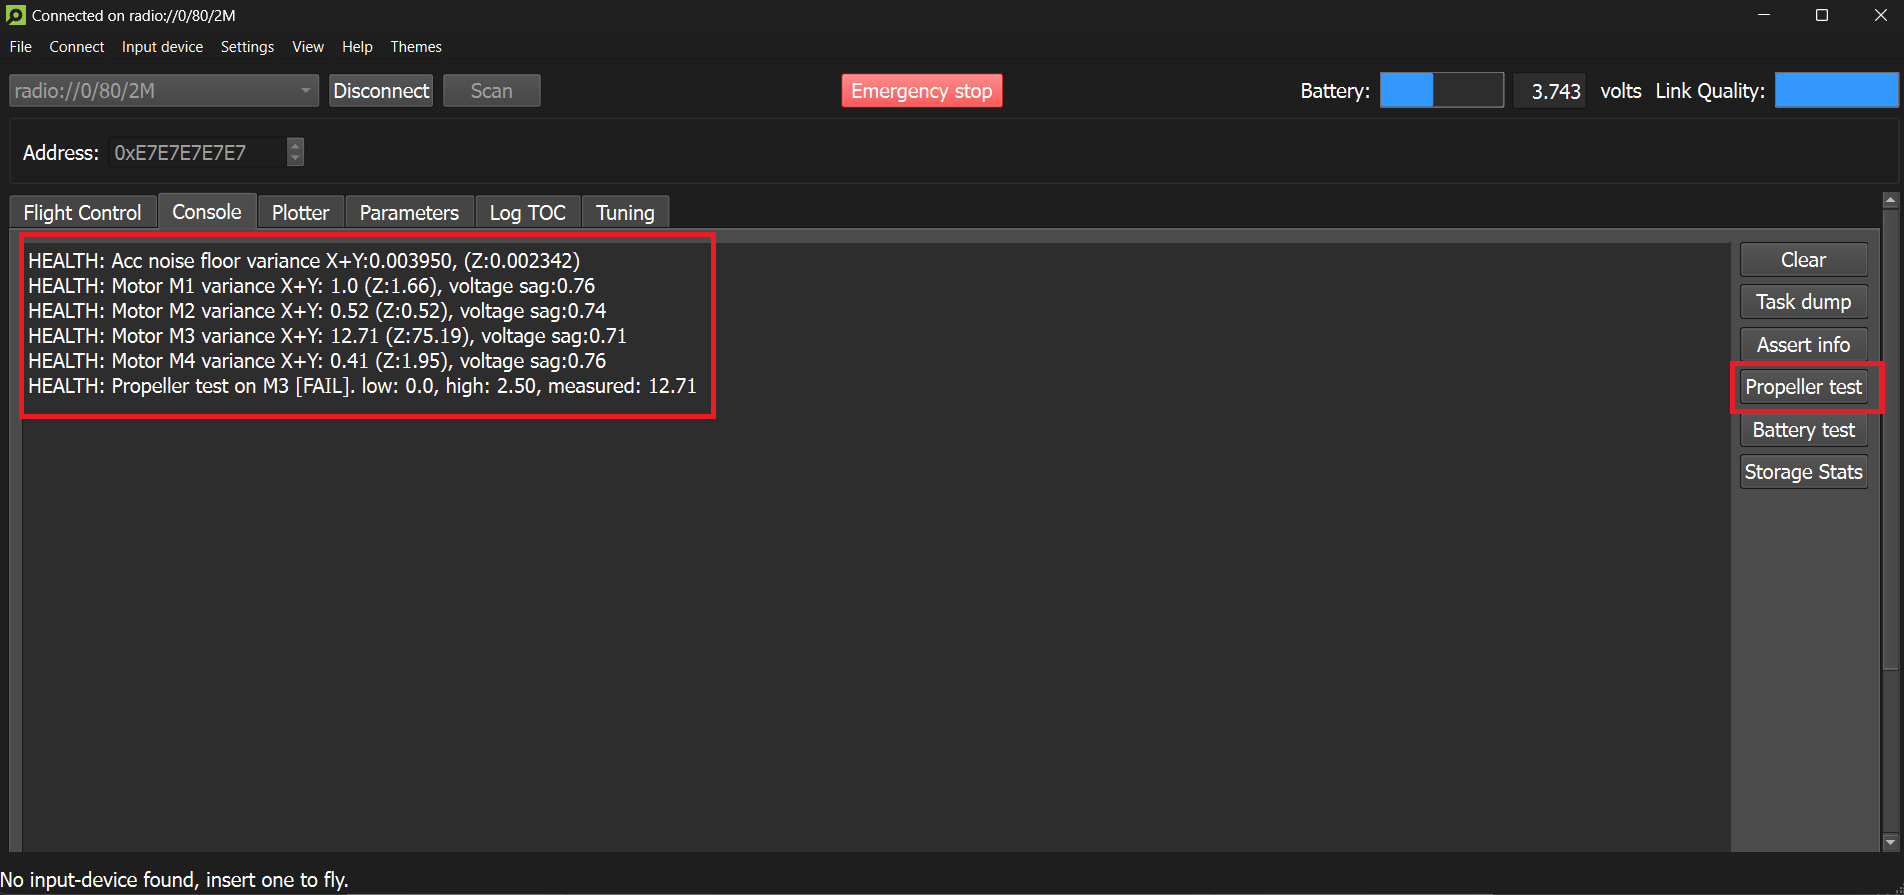
\includegraphics[width=0.85\textwidth]{Propeller_test}
	\caption{Vista de consola y prueba de vibración en hélices y motores.}
	\label{fig:Propeller_test}
\end{figure} 

Las vibraciones excesivas en los motores y hélices perjudican significativamente la calidad de vuelo del dron, por tal motivo fue necesario realizar ajustes para reducirlas o eliminarlas. Hay tres posibles soluciones al problema y deben intentarse en orden:

\begin{enumerate}
	\item \textbf{Balanceo de hélices:} La primera solución para abordar el problema es balancear las hélices, siguiendo el tutorial disponible en la página de Bitcraze \cite{Crazyflie_balancing}.
	
	\item \textbf{Reemplazo de hélices:} Si el balanceo de las hélices no resuelve el problema, se recomienda reemplazarlas con hélices nuevas de repuesto.
	
	\item \textbf{Reemplazo de motores:} Si las vibraciones persisten después de cambiar las hélices, se debe considerar el reemplazo de los motores.
\end{enumerate}

\subsection{Prueba de vuelo simple}
Luego de examinar los aspectos anteriores, se procedió a realizar una prueba de vuelo utilizando la GUI del cfclient y un mando de PS4. El objetivo del experimento fue elevar un poco el dron aplicando una cantidad considerable de Thrust para elevarlo y poder observar su comportamiento en ausencia de un sistema de posicionemiento (lazo abierto). 

El desepgue del dron fue exitoso sin embargo, como se esperaba, no logró mantener su posición durante la elevación presentando una cantidad considerable de drift y descompensación de vuelo.

\section{Instalación de la placa de expansión Flow Deck}
Habiendo verificado el funcionamiento propio del dron Crazyflie y familiarizado con el \textit{software} de control cfclient, se continuó realizando la instalación de la placa de expansión Flow Deck y su validación mediante pruebas de posicionamiento.

\subsection{Montaje y reconocimiento de la placa}
Para proceder con la instalación de la placa de expansión Flow Deck, se siguieron cuidadosamente las instrucciones provistas por Bitcraze en su página oficial \cite{Crazyflie_expansion_decks}. Puede resultar intuitivo, pero es importante mencionar que la placa Flow Deck tiene una orientaión específica para ser instalada. Como se observa en la Figura \ref{fig:FlowDeck_ambas_vistas}, en una de sus vistas tiene indicado que es la vista frontal del sensor y que debe ser orientado hacia arriba. Este lado es el que se acopla directamente sobre el dron Crazyflie utilizando los conectores presentes en la parte inferior del dron. 

\begin{figure}[htbp]
	\centering
	\begin{subfigure}[b]{0.3\textwidth}
		\centering
		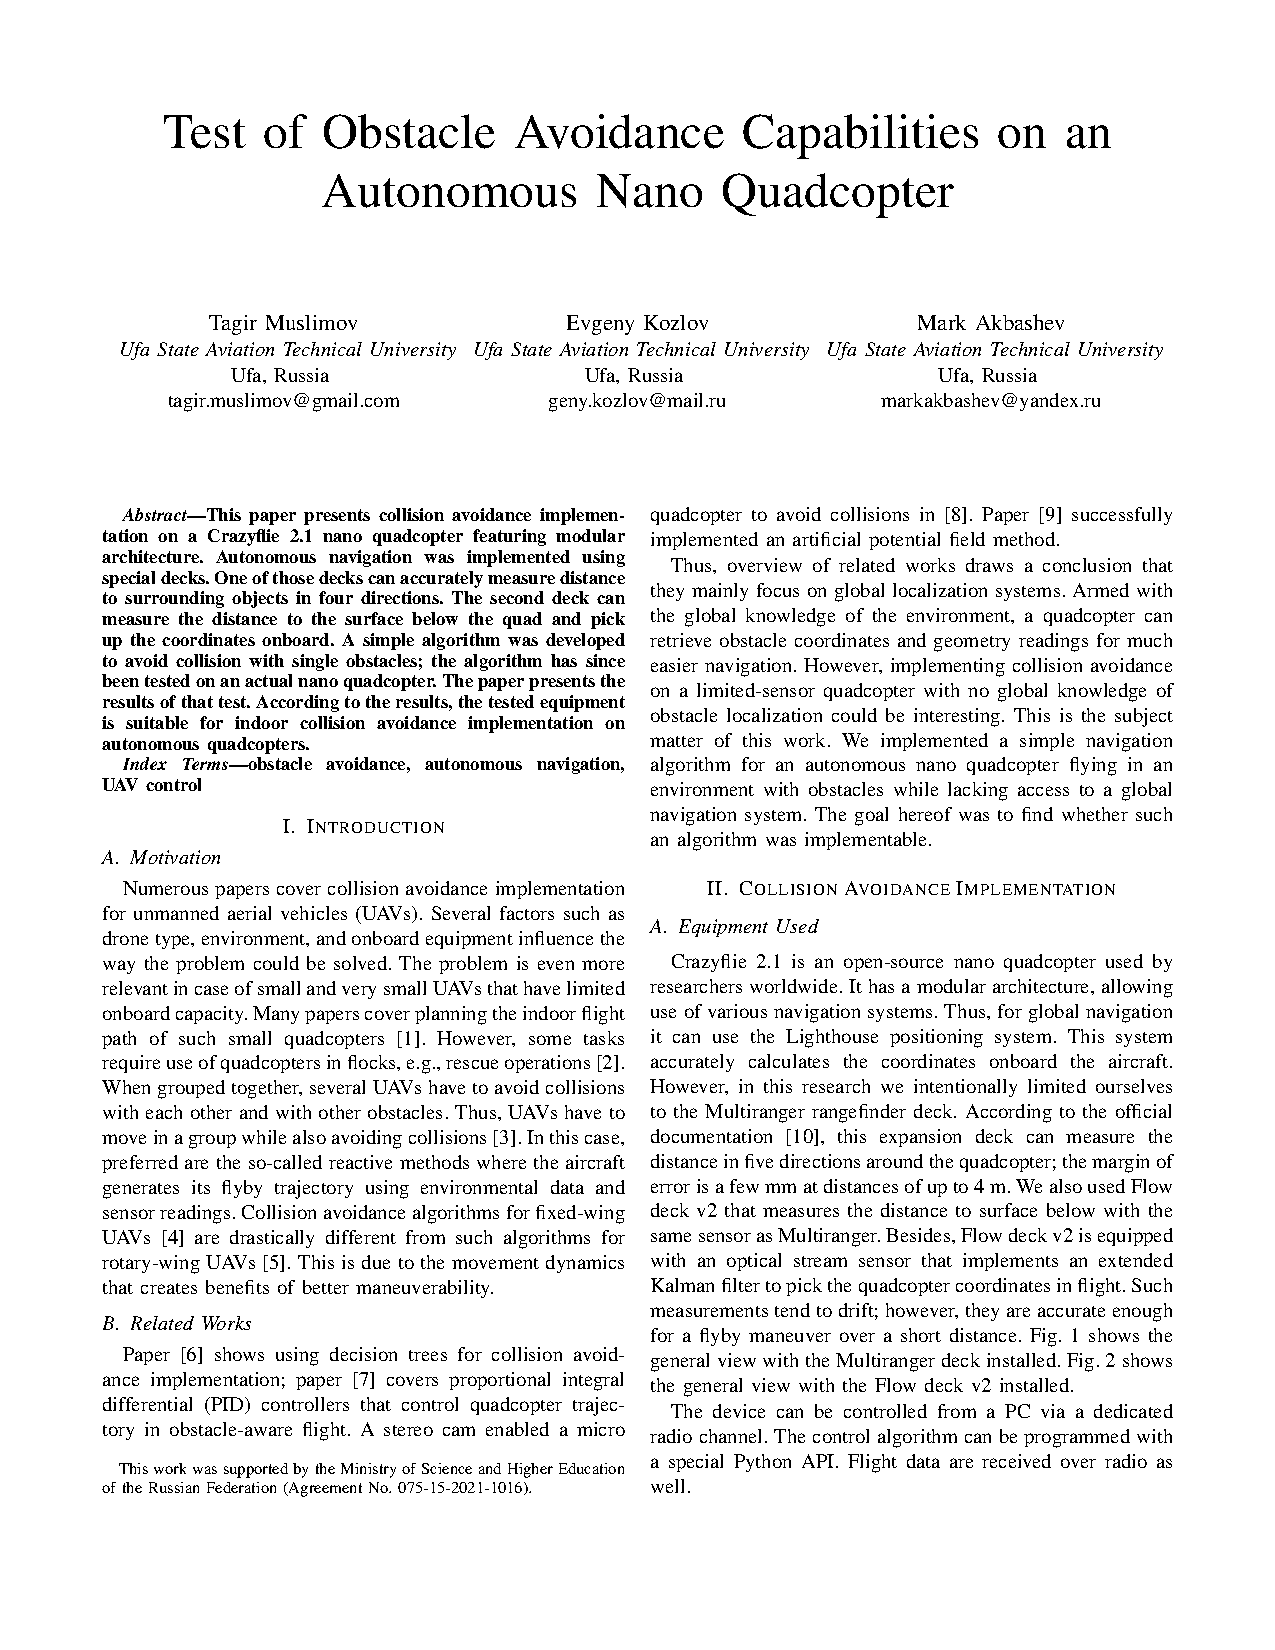
\includegraphics[width=\textwidth]{FlowDeck1}
	\end{subfigure}
	\hspace{0.01\textwidth} % Ajusta el espacio entre las imágenes
	\begin{subfigure}[b]{0.3\textwidth}
		\centering
		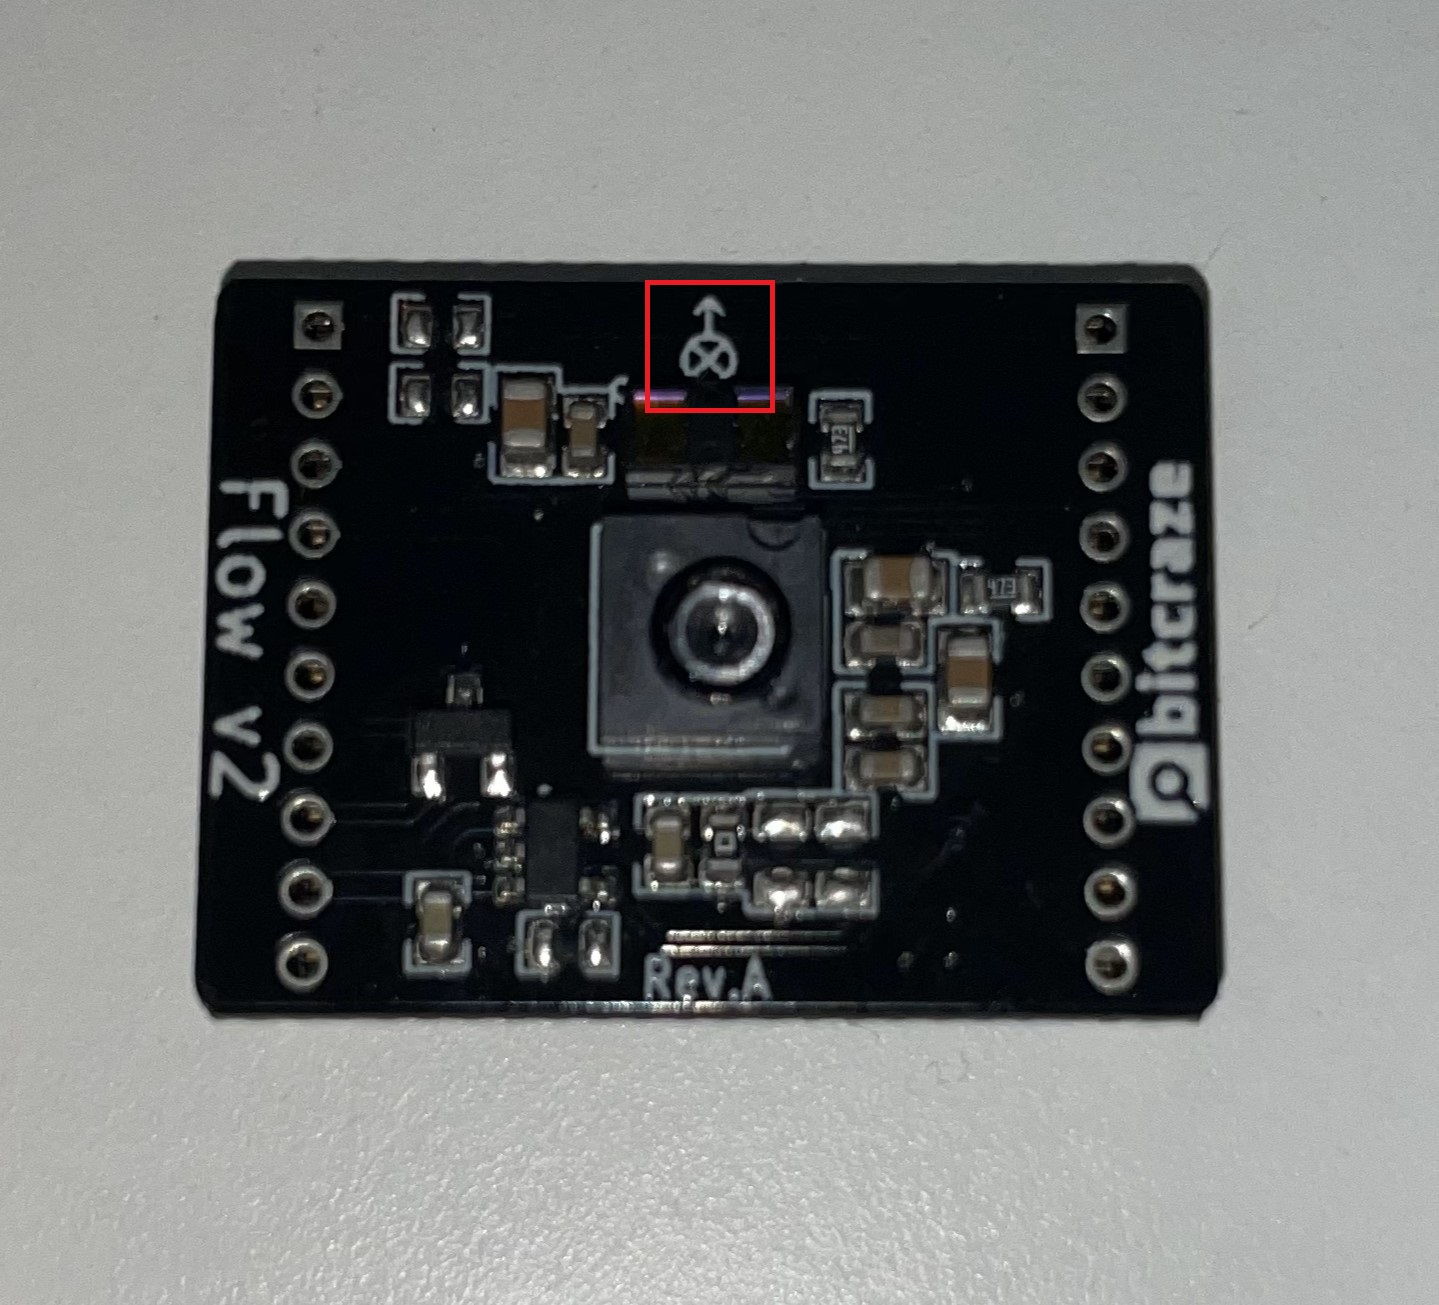
\includegraphics[width=\textwidth]{FlowDeck2}
	\end{subfigure}
	\caption{Vista frontal y trasera de la placa de expansión Flow Deck.}
	\label{fig:FlowDeck_ambas_vistas}
\end{figure}

Además de la orientación, también se debe considerar que la placa tiene una dirección específica para ser instalda. En ambas vistas de la Figura \ref{fig:FlowDeck_ambas_vistas} se observa un símbolo con un círculo y una flecha. Este mismo símbolo se encuentra en la parte inferior del Crazyflie por lo que, al momento de acoplar el sensor, es importante asegurarse que la dirección de los símbolos en ambas placas (Crazyflie y Flow Deck) coincidan, justo como se observa en la Figura \ref{fig:Crazyflie_con_FlowDeck}. De lo contrario, la placa podría experimentar daños irreversibles en el \textit{hardware}.

\begin{figure}[htbp]
	\centering
	\includegraphics[width=0.3\textwidth]{Crazyflie_con_FlowDeck2}
	\caption{Vista inferior del dron Crazyflie con la placa Flow Deck instalada.}
	\label{fig:Crazyflie_con_FlowDeck}
\end{figure} 

El siguiente aspecto que se consideró luego de instalar la placa en el dron fue la verificación de reconocimiento del sensor por parte del \textit{firmware}. Esto se realizó utilizando nuevamente el programa cfclient y conectando el Crazyflie con la placa Flow Deck instalada. 

Una vez conectado el dron al cliente, se consultó la vista de parámetros y en la sección de placas o como aparece en el cliente ``\textit{decks}'', se identificó el registro \textbf{deck.bcFlow2}. Justo como se aprecia en la Figura \ref{fig:FlowDeck_detection2}, este registro es un indicador del reconocimiento de la placa de expansión Flow Deck v2 y como este automáticamente adquirió un valor de 1 se puede asegurar que el Crazyflie detectó exitosamente al sensor.

\begin{figure}[htbp]
	\centering
	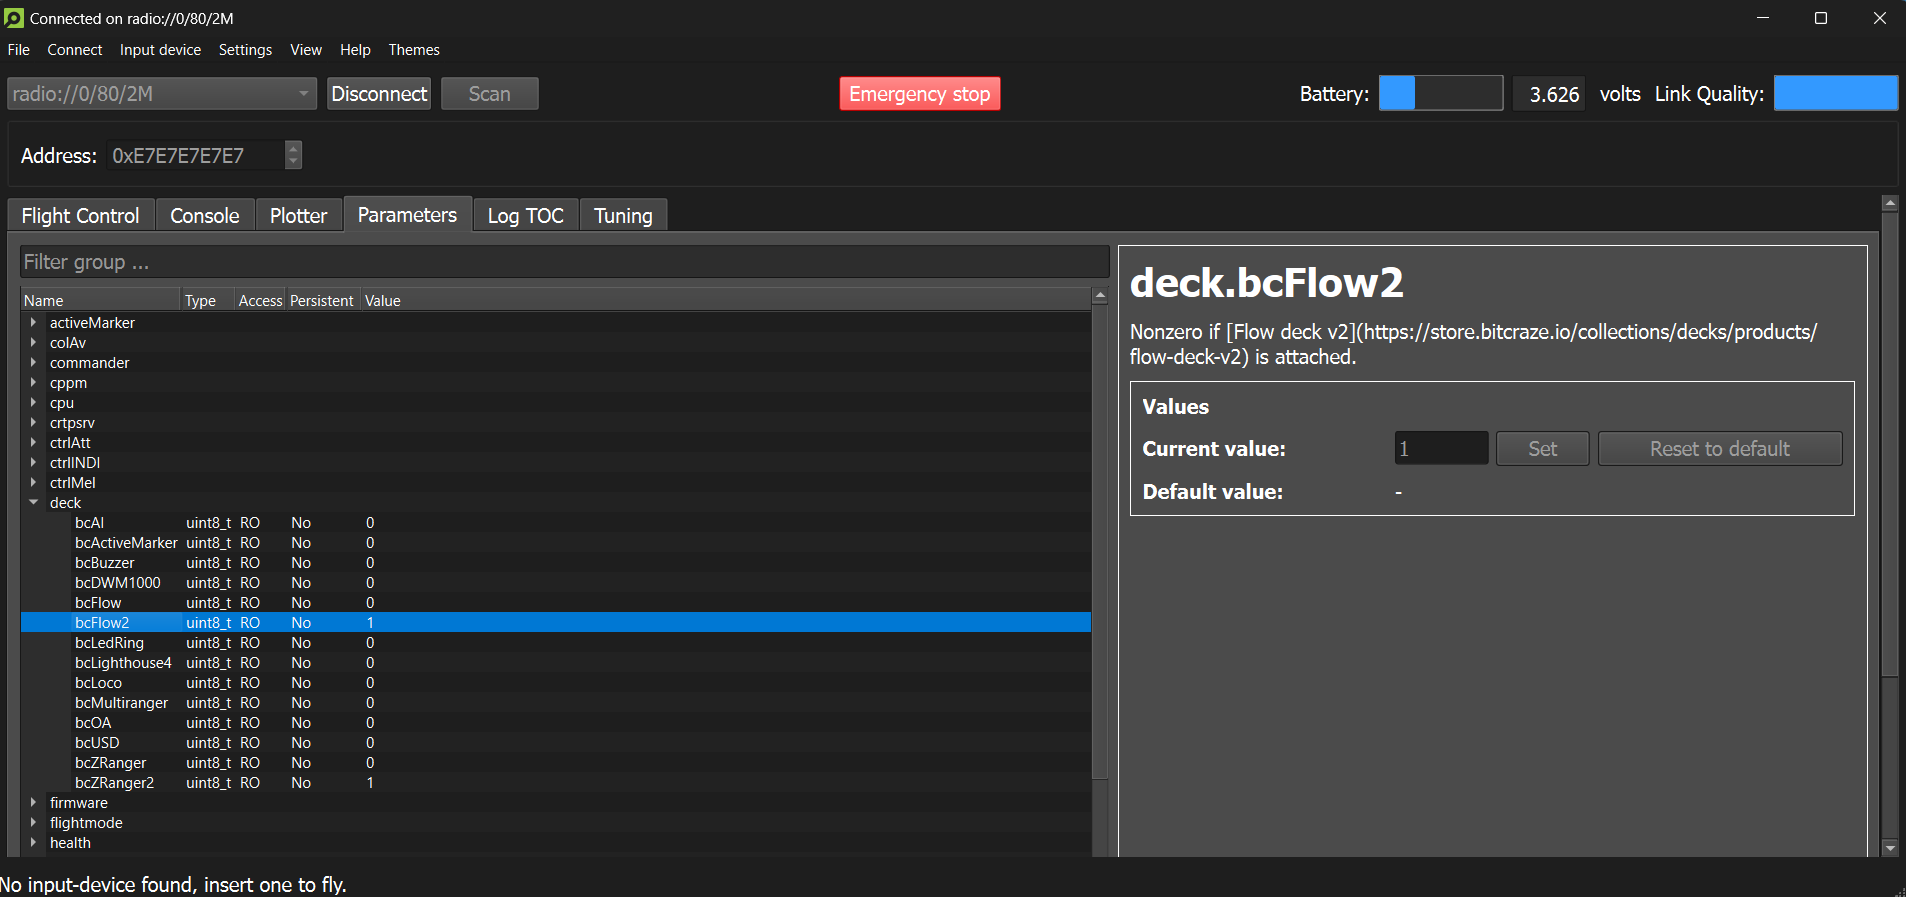
\includegraphics[width=0.85\textwidth]{FlowDeck_detection2}
	\caption{Reconocimiento de placa Flow Deck en vista de parámetros en cfclient.}
	\label{fig:FlowDeck_detection2}
\end{figure} 

Otra forma de identificar si el dron Crazyflie ha detectado a la placa Flow Deck es observar si en la vista de control de vuelo se habilitó el modo asistido flotante o bien, si se habilitaron los controles de vuelo basado en comandos (ver Figura \ref{fig:FlowDeck_detection1}). 

\begin{figure}[htbp]
	\centering
	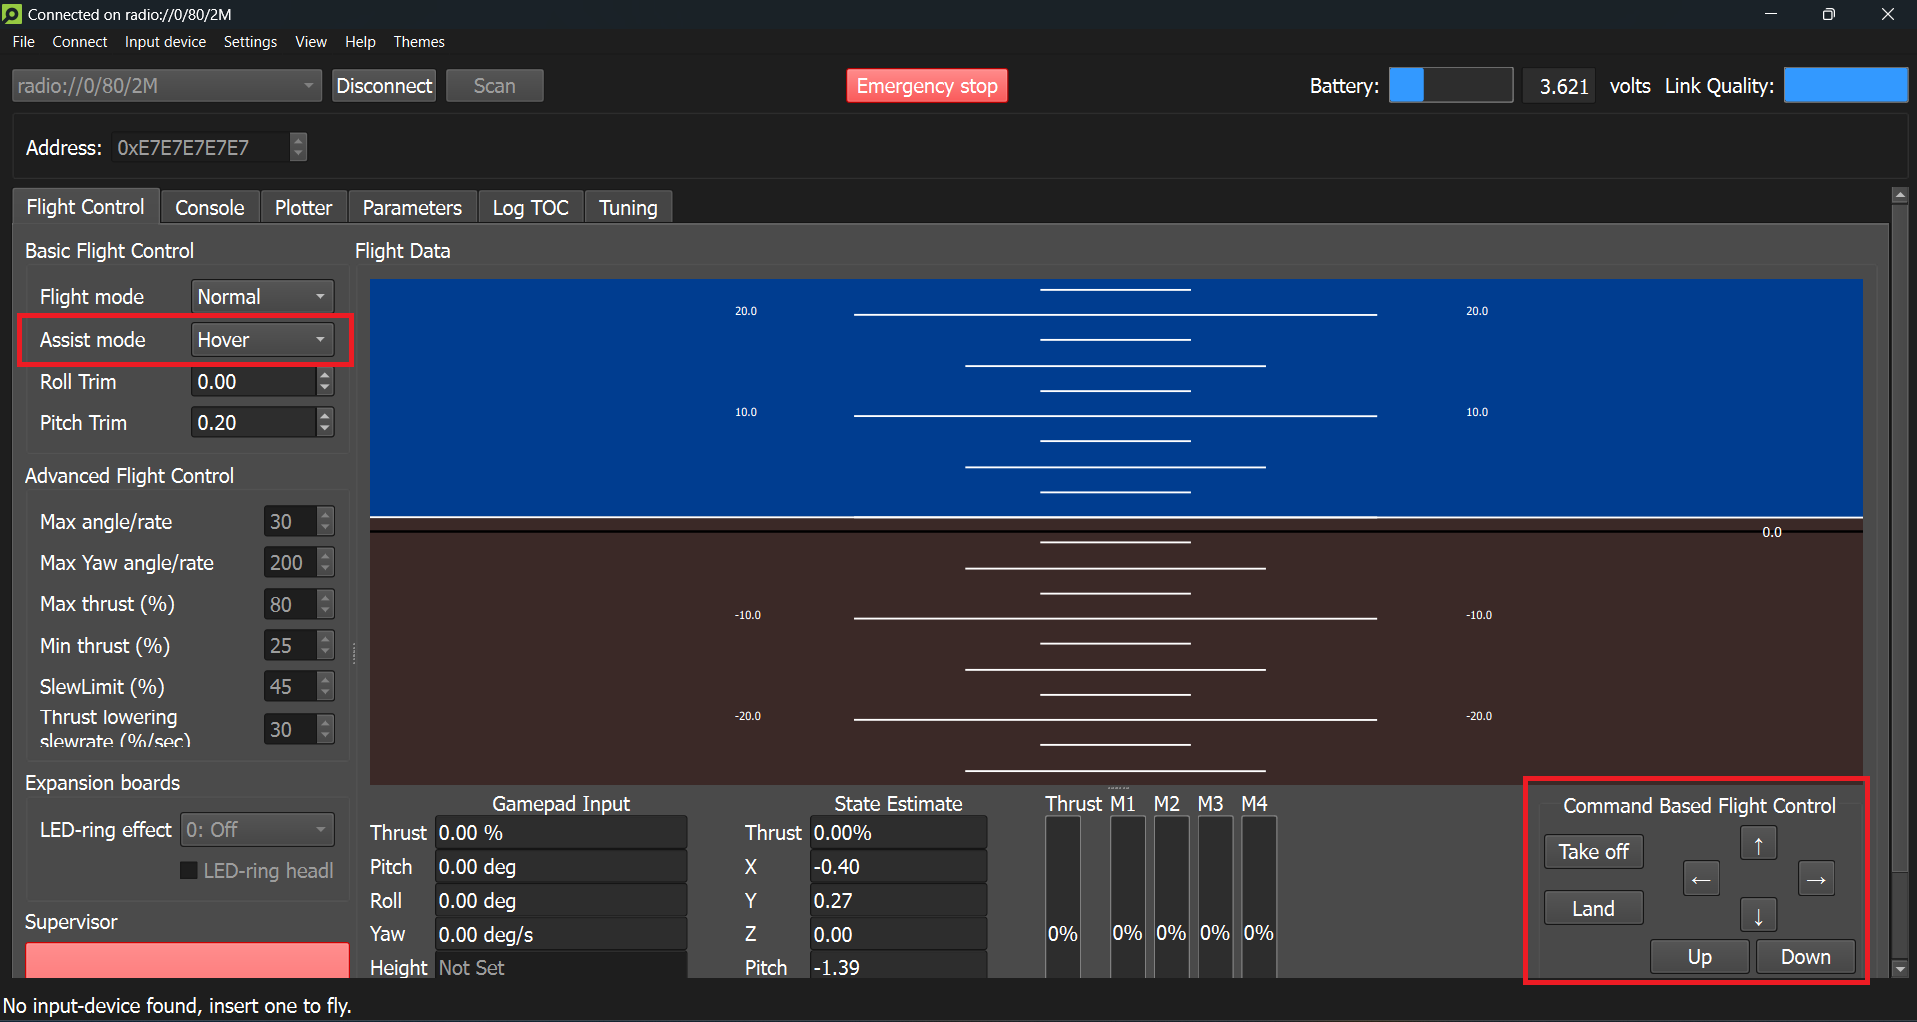
\includegraphics[width=0.85\textwidth]{FlowDeck_detection1}
	\caption{Reconocimiento de placa Flow Deck en vista de control de vuelo en cfclient.}
	\label{fig:FlowDeck_detection1}
\end{figure} 
 
\subsection{Pruebas de posicionamiento}
Luego de verificar que la placa Flow Deck había sido reconocida por el dron, se procedió a realizar pruebas de vuelo enfocadas en evaluar la mejora en el posicionamiento y estabilidad del dron. El objetivo de estas pruebas fue comparar el desempeño del Crazyflie con y sin la placa de expansión.

Tal como se realizó el experimento sin la placa, la prueba únicamente consistió en elevar el dron a cierta altura y mantenerlo levitando por algunos segundos para despues aterrizarlo. Para ello, el dron se colocó en una superficie plana y, a diferencia de las pruebas sin placa, en estas ya no fue necesario un mando pues se encontraban habilitados los controles de vuelo basados en comandos en la GUI del cfclient (como se observó en la Figura \ref{fig:FlowDeck_detection1}). Y, utilizando el comando ``\textit{take off}'' se logró despegar al dron y este mantuvo una altura constante hasta que se envió el comando ``\textit{land}'' para aterrizarlo. 

\begin{figure}[htbp]
	\centering
	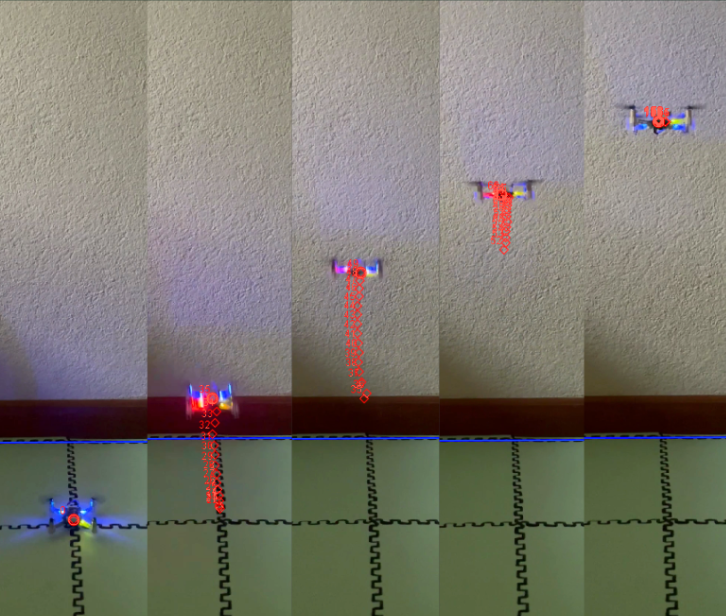
\includegraphics[width=0.5\textwidth]{Prueba_2}
	\caption{Prueba de vuelo y posicionamiento con placa Flow Deck integrada.}
	\label{fig:Prueba_2}
\end{figure} 

Justo como se observa en la Figura anterior \ref{fig:Prueba_2}, el desempeño de vuelo del dron es significativamente mejor que el obtenido para la misma prueba pero sin la placa de posicionamiento. Validando su instalación y reconocmiento en el \textit{firmware} del dron.
 
 
\section{Adaptación de entorno}
Al realizar las pruebas de posicionamiento con la placa Flow Deck, se observó que para distintas condiciones del entorno y para diferentes superficies el comportamiento de posicionamiento del dron Crazyflie fue variable. Esto se debió a las características de los sensores en la placa que mejoran funcionamiento en condiciones específicas. Por ello, surgió la necesidad de identificar un entorno de pruebas con las condiciones óptimas para el correcto desempeño de la placa Flow Deck. 

\subsection{Superficies y condiciones desfavorables}
Durante las pruebas realizadas, se observaron dificultades en la capacidad del dron para mantener su posición cuando se encontraba volando sobre superficies con condiciones de alta reflectividad, demasiada homogeneidad y con condiciones de luz intensas. 
\begin{itemize} 
	\item La homogeneidad en las superficies representó un problema en el desempeño del dron debido a que el sensor de flujo óptico de la placa no era capaz de interpretar movimiento relativo al no identificar diferencias significativas en las imágenes de la superficie.
	\item La condición de luz intensa con sombras muy marcadas también afectó al sensor de flujo óptico, ya que la propia sombra del dron sobre la superficie generaba errores en el cálculo de movimiento relativo.
	\item La reflectividad en las superficies perjudicó el funcionamiento del sensor infrarrojo de la placa, provocando que esta no determinara correctamente el movimiento relativo por no tener una lectura correcta de la posición vertical del dron.
\end{itemize}

\vspace{0.7cm}

\begin{figure}[htbp]
	\centering
	\begin{subfigure}[b]{0.26\textwidth}
		\centering
		\includegraphics[width=\textwidth]{superficie1}
	\end{subfigure}
	\hspace{0.01\textwidth} % Ajusta el espacio entre las imágenes
	\begin{subfigure}[b]{0.26\textwidth}
		\centering
		\includegraphics[width=\textwidth]{superficie2}
	\end{subfigure}
	\label{fig:Superficies_probadas1}
\end{figure}

\begin{figure}[htbp]
	\centering
	\begin{subfigure}[b]{0.26\textwidth}
		\centering
		\includegraphics[width=\textwidth]{superficie3}
	\end{subfigure}
	\hspace{0.01\textwidth} % Ajusta el espacio entre las imágenes
	\begin{subfigure}[b]{0.27\textwidth}
		\centering
		\includegraphics[width=\textwidth]{superficie4}
	\end{subfigure}
	\caption{Superficies de prueba con pésimos resultados debido a condiciones anteriormente descritas.}
	\label{fig:Superficies_probadas2}
\end{figure}

En la Figura \ref{fig:Superficies_probadas2} se muestran algunas de las superficies que fueron probadas. La primer imagen es en la superficie natural del ecosistema Robotat, pero la homogeneidad de la superficie presentó un pésimo posicionamiento, provocando que el dron volara erráticamente. La segunda y tercera figura corresponden a papel mate con patrones impresos sin embargo, la pintura utilizada presentó alta reflectividad, lo que produjo que el dron no fuera capaz de estimar correctamente su posición. La última superficie, una alfombra con cubierta impresa de grama artificial presento el mismo problema debido a ser muy reflectiva.

\subsection{Solución de entorno y observaciones}
Para mitigar los problemas de funcionamiento debido a las condiciones del entorno, se tomaron varias medidas. Primero, se ajustó el entorno de vuelo empleando una superficie antirreflejante con patrones visibles, lo que mejoró significativamente la capacidad de los sensores del Flow Deck. Las superficies antirreflejantes utilizadas consistieron en alfombras modulares de foami con patrones situados con pintura antireflejante, justo como se observa en la Figura \ref{fig:Superficie_funcional_1}.  

\vspace{0.25cm}
\begin{figure}[htbp]
	\centering
	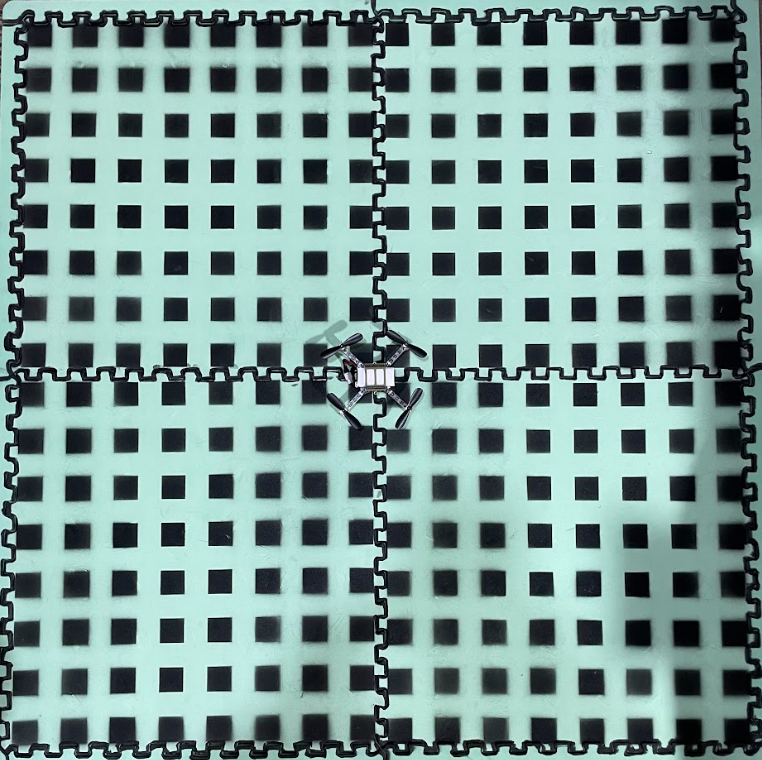
\includegraphics[width=0.6\textwidth]{superficie5}
	\caption{Prototipo de superficie adaptada para el funcionamiento de la placa Flow Deck.}
	\label{fig:Superficie_funcional_1}
\end{figure} 

Estas alfombras pueden ser adaptadas en distintos entornos y resultan especialmente prácticas para ser instaladas en el ecositema Robotat, pues pueden ser colocadas y retiradas con facilidad. Además, al ser de material foami tienen la característica de ser amortiguadoras, ayudando a reducir el daño en el \textit{hardware} del dron en caso de colisiones por fallas o errores.

Otro aspececto importante que se tuvo en consideración fue la ilumincación del entorno. Fue importante asegurarse que la distribución de luz sea adecuada, de forma que se minimice al máximo la propia sombra del dron y para que no termine afectando a las lecturas del sensor de flujo óptico.

Estas mejoras permitieron un rendimiento más estable del dron, asegurando que el Flow Deck pudiera operar de manera óptima. Estas observaciones son fundamentales para futuros experimentos, recomendando realizar vuelos en entornos controlados y adecuadamente preparados para evitar problemas de posicionamiento. 


% ------------------------------------------------------------------------------
% CAPÍTULO 8 -------------------------------------------------------------------
% ------------------------------------------------------------------------------
\chapter{Herramientas de software para control individual de dron Crazyflie}
En este capítulo se presenta el desarrollo e implementación de algoritmos de control básicos para el dron Crazyflie con la placa Flow Deck integrada. Se detallan los pasos de instalación de las dependencias, desarrollo de funciones de control específicas en Python y su implementación desde el entorno de Matlab. Además, se presenta un método para mejorar el rendimiento de vuelo al mezclar las lecturas de posicionamiento de la placa Flow Deck con lecturas de un sistema de captura de movimiento. Por último, se presentan herramientas de simulación para experimentar con el dron Crazyflie, detallando los alcances de estas. 

\section{Algoritmos de control básico en Python}
Con el fin de lograr un control efectivo del dron Crazyflie, se desarrollaron una serie de algoritmos básicos en Python utilizando la librería oficial de Crazyflie en python, cflib. Estos algoritmos permiten ejecutar comandos para conexión, lectura de variables, configuración de parámetros y movimiento básicos de vuelo. Estas proporcionan una base para realizar una amplia variedad de experimentos.

\subsection{Instalación de librería cflib}
La librería Crazyflie es una herramienta fundamental para interactuar y controlar al dron mediante algoritmos en Python. Para su instalación es necesario asegurarse previamente de tener instalada una versión de Python entre las versiones 3.7 y 3.11. Para el desarrollo del proyecto se instaló la versión 3.11.0 disponible para Windows 11 en la página oficial de Python \cite{Python_3_11_0}. Al instalarlo se tomó el cuidado de asegurarse que la ruta a Python estuviera agregada al PATH.

\newpage
Para confirmar la versión de Python instalada en el sistema, se ejecuta el siguiente comando en la terminal de Windows:

\begin{verbatim}
	python --version
\end{verbatim}

El resultado en consola confirma que la versión en uso es la \textbf{3.11.0}, como se muestra en la Figura \ref{fig:cmd_python_version}.

Una vez verificada la versión de Python, se procede a la instalación de cflib mediante el gestor de paquetes pip, ejecutando el siguiente comando:

\begin{verbatim}
	pip install cflib
\end{verbatim}

Al ejecutar este comando, se descargan e instalan automáticamente las dependencias necesarias, como \textbf{pyusb}, \textbf{libusb-package}, \textbf{scipy}, \textbf{numpy}, entre otras. La versión de la librería instalada fue \textbf{cflib-0.1.26}, como se observa en la Figura \ref{fig:cmd_python_version}.

\vspace{0.5cm}
\begin{figure}[htbp]
	\centering
	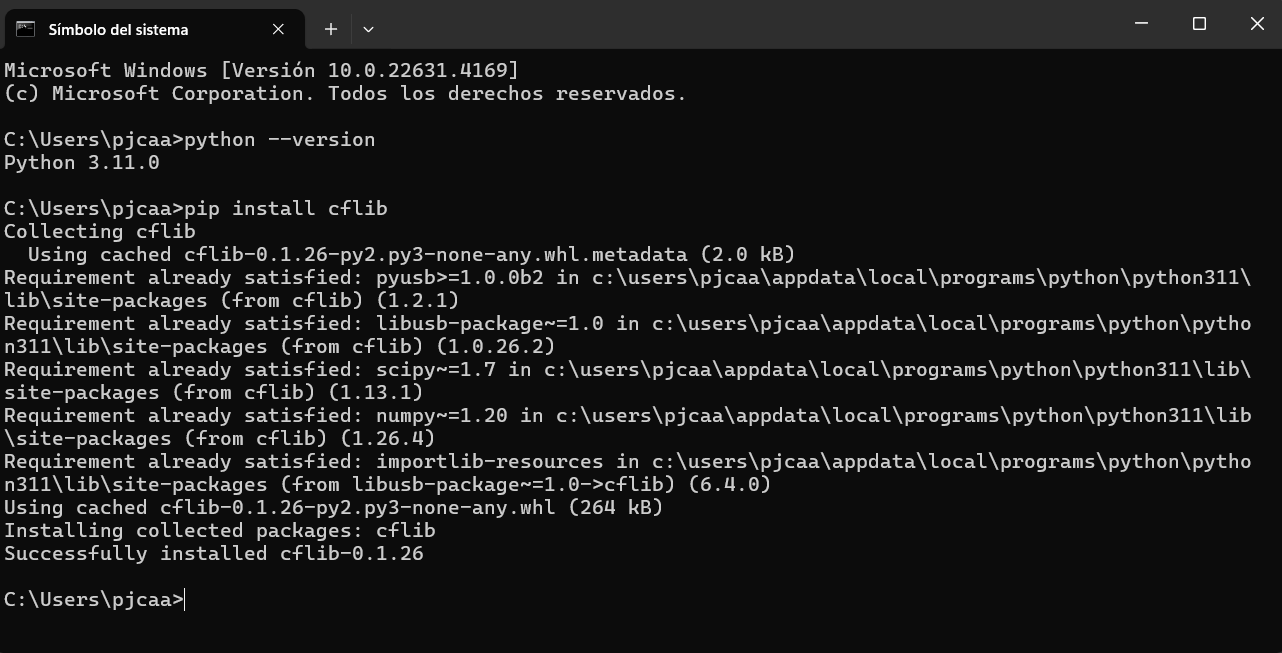
\includegraphics[width=0.9\textwidth]{cmd_python_version}
	\caption{Ejecución de comandos en la terminal de Windows.}
	\label{fig:cmd_python_version}
\end{figure} 
\vspace{0.5cm}

Tras la instalación, se llevaron a cabo pruebas básicas para garantizar que la librería cflib se instaló correctamente y que el dron puede recibir comandos desde un script de Python. Es importante mencionar que, a lo largo de este proyecto se utilizó el programa \textit{Visual Studio Code} como editor de texto para los algoritmos en Python. 

A continuación, se presenta el código de prueba que realiza la conexión y desconexión del dron (ver Código \ref{code:prueba_conexion_crazyflie}). 

\newpage
\begin{lstlisting}[caption=Algoritmo de prueba en Python utilizando la librería Cflib., label=code:prueba_conexion_crazyflie]
	import time
	import cflib.crtp
	from cflib.crazyflie import Crazyflie
	
	# Inicializar los drivers
	cflib.crtp.init_drivers()
	
	# Crear el objeto Crazyflie
	cf = Crazyflie(rw_cache='./cache')
	
	try:
		# Intentar conectar al Crazyflie
		cf.open_link('radio://0/80/2M/E7E7E7E7E7')
		print("Crazyflie conectado.")
		time.sleep(5)  # Espera 5 segundos
	except Exception as e:
		print(f"Ocurrió un error al intentar la conexión: {e}")
	finally:
		# Asegurar la desconexión del Crazyflie
		cf.close_link()
		print("Crazyflie desconectado.")
\end{lstlisting}

El algoritmo presentado realiza un proceso simple de conexión con el dron Crazyflie, manteniendo activa la conexión por 5 segundos para luego cerrar la conexión. Para lograrlo se utilizó la libería time y los módulos CRTP y Crazyflie de la libería cflib. El móudlo CRTP se utilizó para inicializar los drivers para el dispositivo Crazyradio y el módulo Crazyflie se empleó para instanciar un objeto de la clase princial Crazyflie, este fue la representación del dron en el código. En la Figura \ref{fig:algoritmo_prueba_vs}, se muestra el entorno de desarrollo de \textit{VS Code} y la correcta compilación y ejecución del algoritmo de prueba. 

\begin{figure}[htbp]
	\centering
	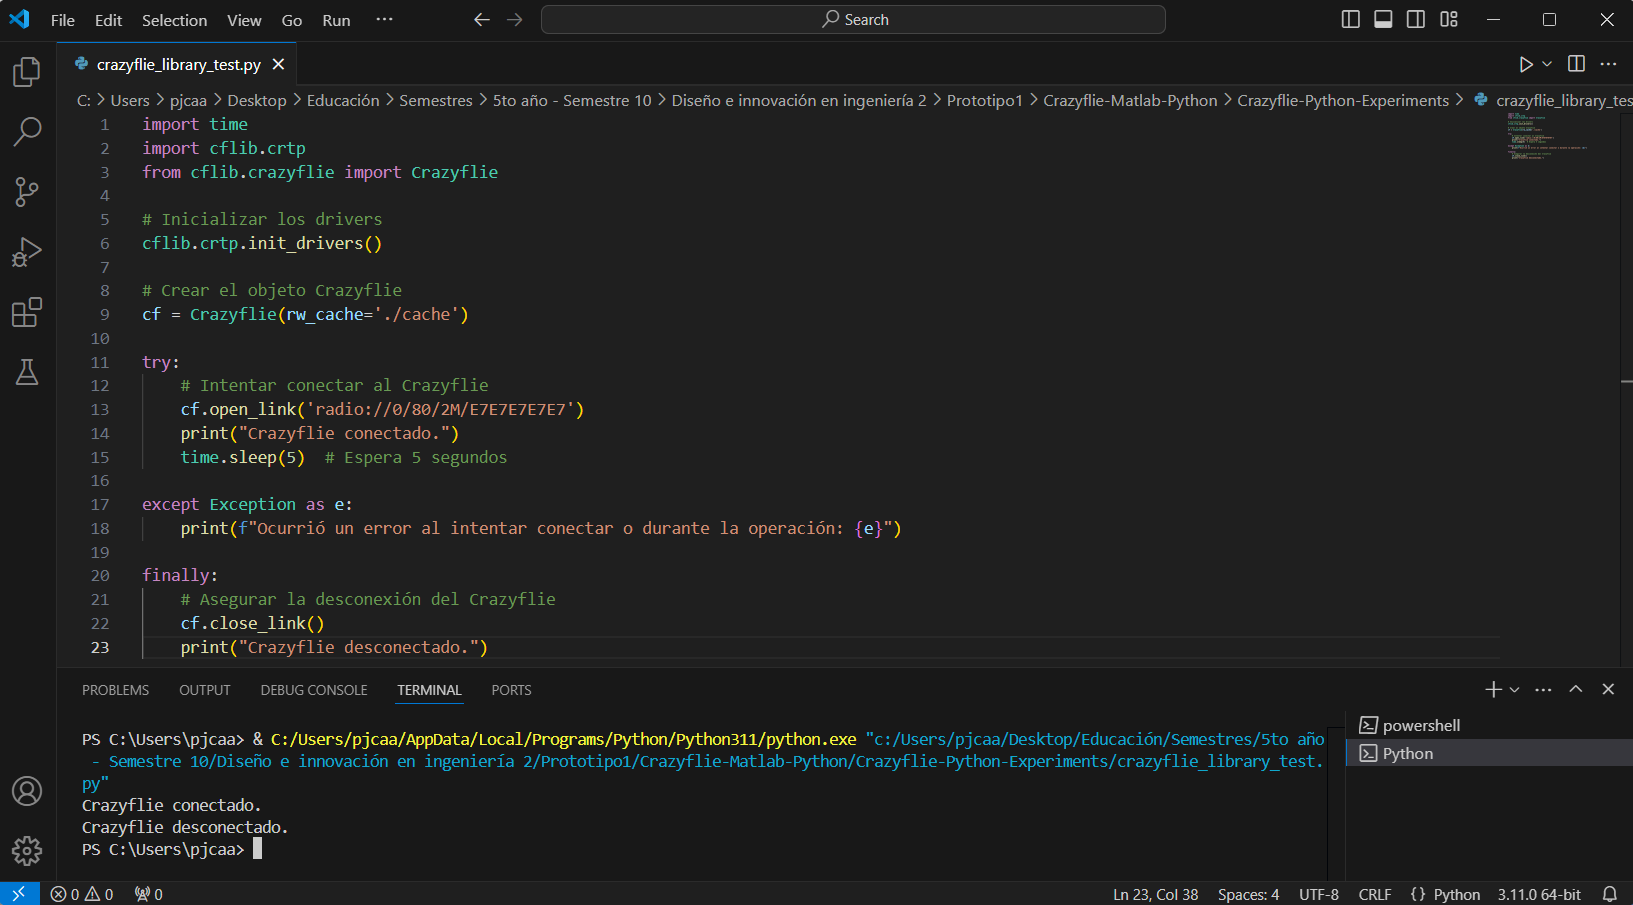
\includegraphics[width=1\textwidth]{algoritmo_prueba_vs}
	\caption{Ejecución de algoritmo de prueba en \textit{Visual Studio Code}.}
	\label{fig:algoritmo_prueba_vs}
\end{figure}

\newpage
\subsection{Uso de librería cflib y recursos adicionales}
Para el desarrollo de los algoritmos de control se utilizaron módulos específicos de la librería cflib para Crazyflie y algunas librerías estándar de python. A continuación, se detallan las librerías y módulos utilizados y su propósito:

\subsubsection{Módulos de cflib utilizados}

\begin{itemize}
	\item \textbf{CRTP:} El módulo cflib.crtp es responsable de inicializar los drivers necesarios para la comunicación mediante el protocolo \textit{Crazy Real-Time Protocol}, utilizado para establecer la conexión con el dron a través del dispositivo Crazyradio.
	\item \textbf{Crazyflie:} El módulo cflib.crazyflie es la interfaz que permite controlar y comunicarse con el dron. 
	\begin{itemize}
		\item Submódulo Log: El submódulo cflib.crazyflie.log se empleó para configurar los registros de variables en tiempo real.
		\item Submódulo SyncCrazyflie: El submódulo cflib.crazyflie.synccrazyflie se empleó para simplificar el manejo de conexiones mediante el uso de la subclase SyncCrazyflie. 
		\item Submódulo HighLevelCommander: El submódulo cflib.crazyflie.high\_level\_commander se empleó como una interfaz de alto nivel para el envío de comandos de control de vuelo hacia el dron. 
	\end{itemize}
\end{itemize} 

Es importante mencionar que se utilizó la versión síncrona de la librería Crazyflie en lugar de la versión asíncrona, como se evidencia en el uso de la subclase SyncCrazyflie. Esta convierte a las funciones no bloqueantes de la versión asíncrona en funciones bloqueantes, lo que significa que el programa espera a que una tarea termine antes de continuar con la siguiente.

Esta elección se realizó por la necesidad de ejecutar comandos de control de manera secuencial y confiable. Al utilizar una versión síncrona, se asegura que cada acción enviada sea completada antes de ejecutar la siguiente. De esta forma el dron puede completar algoritmos de forma secuencial, tal como se esperaría para un algoritmo de seguimiento de trayectorias.

\subsubsection{Recursos adicionales de Python utilizados}
\begin{itemize}
	\item \textbf{logging:} Se utilizó para configurar el nivel de registro de mensajes dentro del programa. 
	\item \textbf{time:} Se utilizó para realizar gestión de tiempo en la ejecución de las funciones de control. Esto asegurpo que el dron tuviera el tiempo suficiente para ejecutar las acciones solicitadas previo al siguiente comando.
	\item \textbf{sys:} Se utilizó para forzar la salida inmediata de los mensajes en la consola. Esto evitó que el sistema almacenara mensajes en \textit{buffer} y retrasara su impresión en consola.
	\item \textbf{threading:} Se utilizó la clase \textit{Event} del módulo para sincronizar la recepción de datos del dron.
\end{itemize} 

\subsection{Desarrollo de algoritmos de control}
A continuación, se presentan las funciones desarrolladas en python con algoritmos de control de funcionalidades básicas del dron Crazyflie. Están clasificadas en cuatro grupos: conexión, lectura de variables, configuración de parámetros y movimiento general.

\subsubsection{Funciones de conexión}
\begin{itemize}
	\item \textbf{connect(uri)} \ref{code:funcion_connect} \\ 
	Esta función se utiliza para establecer y mantener una conexión activa con el dron Crazyflie de manera síncrona. Requiere que sea especificado el Identificador Unifrome de Recursos (URI) del Crazyflie objetivo . 
	\begin{itemize}
		\item Atributos:
		\begin{itemize}
			\item \texttt{uri} (\texttt{str}): Dirección URI del Crazyflie a conectar.
		\end{itemize}
		\item Valor de retorno:
		\begin{itemize}
			\item Retorna una instancia de la clase \texttt{SyncCrazyflie} si la conexión es exitosa.
			\item Imprime en consola un mensaje de confirmación de conexión o de alerta de error con los detalles correspondientes.
		\end{itemize}
	\end{itemize} 

	\item \textbf{disconnect(SyncCrazyflie)} \ref{code:funcion_disconnect} \\ 
	Esta función se utiliza para cerrar la conexión activa con el dron Crazyflie. Requiere que sea especificada la instancia de la clase \texttt{SyncCrazyflie} generada al conectarse . 
	\begin{itemize}
		\item Atributos:
		\begin{itemize}
			\item \texttt{SyncCrazyflie} (\texttt{scf}): Instancia de la clase \texttt{SyncCrazyflie} generada al establecer la conexión.
		\end{itemize}
		\item Valor de retorno:
		\begin{itemize}
			\item Imprime en consola un mensaje de confirmación de desconexión o de alerta de error con los detalles correspondientes.
		\end{itemize}
	\end{itemize} 
\end{itemize}

\subsubsection{Funciones de lectura de variables}
\begin{itemize}
	\item \textbf{get\_pose(SyncCrazyflie)} \ref{code:funcion_get_pose}\\ 
	Esta función se utiliza para obtener los valores actuales de los registros de la estimación de posición del dron Crazyflie.
	\begin{itemize}
		\item Atributos:
		\begin{itemize}
			\item \texttt{SyncCrazyflie} (\texttt{scf}): Instancia de la clase \texttt{SyncCrazyflie} generada al establecer la conexión.
		\end{itemize}
		\item Valor de retorno:
		\begin{itemize}
			\item Retorna un diccionario con los valores de posición actuales del Crazyflie. Las llaves del diccionario correspondiente son: 'x', 'y', 'z', 'roll', 'pitch', 'yaw'.
			\item Imprime en consola un mensaje con los valores de posición actual o un mensaje de alerta de error con los detalles correspondientes.
		\end{itemize}
	\end{itemize} 
	\vspace{1mm} % Espacio adicional entre funciones
	\item \textbf{get\_pid\_values(SyncCrazyflie)} \ref{code:funcion_get_pid_values}\\ 
	Esta función se utiliza para obtener los valores actuales de los registros de los controladores PID de posición del Crazyflie.
	\begin{itemize}
		\item Atributos:
		\begin{itemize}
			\item \texttt{SyncCrazyflie} (\texttt{scf}): Instancia de la clase \texttt{SyncCrazyflie} generada al establecer la conexión.
		\end{itemize}
		\item Valor de retorno:
		\begin{itemize}
			\item Retorna un diccionario con los valores actuales de los controladores PID de posición  del Crazyflie. Las llaves del diccionario correspondiente son: 'X', 'Y', 'Z' y cada una posee un arreglo con las constantes P, I y D.
			\item Imprime en consola un mensaje con los valores actuales de los controladores PID de posición o un mensaje de alerta de error con los detalles correspondientes.
		\end{itemize}
	\end{itemize} 
	\vspace{1mm} % Espacio adicional entre funciones
	
	\item \textbf{get\_pid\_x(scf)}, \textbf{get\_pid\_y(scf)} y \textbf{get\_pid\_z(scf)} \ref{code:funcion_get_pid_x}\\
	Estas funcones se utilizan para obtener los valores actuales del controlador PID de posición en el eje correspondiente del dron Crazyflie.
	\begin{itemize}
		\item Atributos:
		\begin{itemize}
			\item \texttt{SyncCrazyflie} (\texttt{scf}): Instancia de la clase \texttt{SyncCrazyflie} generada al establecer la conexión.
		\end{itemize}
		\item Valor de retorno:
		\begin{itemize}
			\item Retorna un arreglo con los valores actuales de las tres constantes del controlador PID de posición del eje correspondiente.
			\item Imprime en consola un mensaje con los valores del controlador PID de posición del eje correspondiente o un mensaje de alerta de error con los detalles correspondientes.
		\end{itemize}
	\end{itemize}
	\vspace{1mm} % Espacio adicional entre funciones
	
	\item \textbf{detect\_flow\_deck(SyncCrazyflie)} \ref{code:funcion_detect_flow_deck}\\ 
	Esta función se utiliza verificar que el dron Crazyflie conectado esté detectando correctamente a la placa de expansión Flow Deck. Fue desarrollada como una función de prevención de accidentes, ya que si no se detecta dicha placa el comportamiento del dron Crazyflie es errático. 
	\begin{itemize}
		\item Atributos:
		\begin{itemize}
			\item \texttt{SyncCrazyflie} (\texttt{scf}): Instancia de la clase \texttt{SyncCrazyflie} generada al establecer la conexión.
		\end{itemize}
		\item Valor de retorno:
		\begin{itemize}
			\item Retorna un valor True si se detecta correctamente la placa Flow Deck y False si esta no es detectada. 
			\item Imprime en consola un mensaje confimando o negando la detección de la placa de expansión Flow Deck.
		\end{itemize}
	\end{itemize} 
	\vspace{5mm} % Espacio adicional entre funciones 
\end{itemize}

\subsubsection{Funciones de configuración de parámetros}
\begin{itemize}
	\item \textbf{set\_position(SyncCrazyflie, x, y, z)} \ref{code:funcion_set_position}\\ 
	Esta función se utiliza para configurar el valor en los registros de la estimación de posición del dron Crazyflie. Es decir, actualiza la posición actual en el marco de referencia relativo del dron Crazyflie.
	\begin{itemize}
		\item Atributos:
		\begin{itemize}
			\item \texttt{SyncCrazyflie} (\texttt{scf}): Instancia de la clase \texttt{SyncCrazyflie} generada al establecer la conexión.
			\item \texttt{x} (\texttt{float}): Coordenada X en metros de la posición a configurar.
			\item \texttt{y} (\texttt{float}): Coordenada Y en metros de la posición a configurar.
			\item \texttt{z} (\texttt{float}): Coordenada Z en metros de la posición a configurar.
		\end{itemize}
		\item Valor de retorno:
		\begin{itemize}
			\item Imprime en consola un mensaje de confirmación de actualización de posición relativa o un mensaje de alerta de error con los detalles correspondientes.
		\end{itemize}
	\end{itemize} 
	\vspace{1mm} % Espacio adicional entre funciones
	
	\item \textbf{set\_pid\_values(SyncCrazyflie, p\_gains, i\_gains, d\_gains)} \ref{code:funcion_set_pid_values}\\ 
	Esta función se utiliza para configurar los valores actuales de los registros de los controladores PID de posición del Crazyflie.
	\begin{itemize}
		\item Atributos:
		\begin{itemize}
			\item \texttt{SyncCrazyflie} (\texttt{scf}): Instancia de la clase \texttt{SyncCrazyflie} generada al establecer la conexión.
			\item \texttt{p\_gains} (\texttt{diccionario}): Diccionario con constantes proporcionales de los controladores PID de posición para los ejes XYZ. Las llaves del diccionario deben ser: 'X', 'Y' y 'Z'.
			\item \texttt{i\_gains} (\texttt{diccionario}): Diccionario con constantes integrativas de los controladores PID de posición para los ejes XYZ. Las llaves del diccionario deben ser: 'X', 'Y' y 'Z'.
			\item \texttt{d\_gains} (\texttt{diccionario}): Diccionario con constantes derivativas de los controladores PID de posición para los ejes XYZ. Las llaves del diccionario deben ser: 'X', 'Y' y 'Z'.
		\end{itemize}
		\item Valor de retorno:
		\begin{itemize}
			\item Imprime en consola un mensaje de confirmación de actualización de constantes de controladores PID de posición o un mensaje de alerta de error con los detalles correspondientes.
		\end{itemize}
	\end{itemize} 
	\vspace{1mm} % Espacio adicional entre funciones
	
	\item \textbf{set\_pid\_x(scf, P, I, D)}, \textbf{set\_pid\_y(scf, P, I, D)} y \textbf{set\_pid\_z(scf, P, I, D)} \ref{code:funcion_set_pid_x} \\
	Estas funciones se utilizan para configurar los valores de las constantes del controlador PID de posición en el eje correspondiente del dron Crazyflie.
	\begin{itemize}
		\item Atributos:
		\begin{itemize}
			\item \texttt{SyncCrazyflie} (\texttt{scf}): Instancia de la clase \texttt{SyncCrazyflie} generada al establecer la conexión.
			\item \texttt{P} (\texttt{float}): Constante proporcional para el controlador PID de posición del eje correspondiente.
			\item \texttt{I} (\texttt{float}): Constante integrativa para el controlador PID de posición del eje correspondiente.
			\item \texttt{D} (\texttt{float}): Constante derivativa para el controlador PID de posición del eje correspondiente.
		\end{itemize}
		\item Valor de retorno:
		\begin{itemize}
			\item Imprime en consola un mensaje con los valores del controlador PID de posición del eje correspondiente o un mensaje de alerta de error con los detalles correspondientes.
		\end{itemize}
	\end{itemize} 
\end{itemize}

\subsubsection{Funciones de movimiento}
\begin{itemize}
		\item \textbf{takeoff(SyncCrazyflie, height, duration)} \ref{code:funcion_takeoff}\\ 
	Esta función se utiliza para realizar el despegue del dron Crazyflie a una altura dada durante una duración especificada. En caso de no ser especificados la altura y duración, se utilizan los valores por defecto de 0.3 metros y 1 segundo.
	\begin{itemize}
		\item Atributos:
		\begin{itemize}
			\item \texttt{SyncCrazyflie} (\texttt{scf}): Instancia de la clase \texttt{SyncCrazyflie} generada al establecer la conexión.
			\item \texttt{height} (\texttt{float}): Altura en metros que alcanzará durante el despegue. 
			\item \texttt{duration} (\texttt{float}): Tiempo en segundos que tardará en alcanzar la altura de despegue indicada.
		\end{itemize}
		\item Valor de retorno:
		\begin{itemize}
			\item Imprime en consola un mensaje de confirmación de despegue completado o de alerta de error con los detalles correspondientes.
		\end{itemize}
	\end{itemize} 
	\vspace{5mm} % Espacio adicional entre funciones
	
	\item \textbf{land(SyncCrazyflie, height, duration)} \ref{code:funcion_land}\\ 
	Esta función se utiliza para realizar el aterrizaje del dron Crazyflie a una altura dada durante una duración especificada. En caso de no ser especificados la altura y duración, se utilizan los valores por defecto de 0 metros y 2 segundos.
	\begin{itemize}
		\item Atributos:
		\begin{itemize}
			\item \texttt{SyncCrazyflie} (\texttt{scf}): Instancia de la clase \texttt{SyncCrazyflie} generada al establecer la conexión.
			\item \texttt{height} (\texttt{float}): Altura en metros que alcanzará durante el despegue. 
			\item \texttt{duration} (\texttt{float}): Tiempo en segundos que tardará en alcanzar la altura de aterrizaje indicada.
		\end{itemize}
		\item Valor de retorno:
		\begin{itemize}
			\item Imprime en consola un mensaje de confirmación de aterrizaje completado o de alerta de error con los detalles correspondientes.
		\end{itemize}
	\end{itemize} 
	\vspace{5mm} % Espacio adicional entre funciones
	
	\item \textbf{move\_to\_position(SyncCrazyflie, x, y, z, velocity)} \ref{code:funcion_move_to_position}\\ 
	Esta función se utiliza para mover al dron a una posición nueva con una velocidad dada. Requiere de las coordenadas XYZ de la nueva posición y la velocidad del movimiento. La velocidad puede ser omitida y toma el valor por defecto de 1 metro por segundo. 
	\begin{itemize}
		\item Atributos:
		\begin{itemize}
			\item \texttt{SyncCrazyflie} (\texttt{scf}): Instancia de la clase \texttt{SyncCrazyflie} generada al establecer la conexión.
			\item \texttt{x} (\texttt{float}): Coordenada X en metros de la nueva posición.
			\item \texttt{y} (\texttt{float}): Coordenada Y en metros de la nueva posición.
			\item \texttt{z} (\texttt{float}): Coordenada Z en metros de la nueva posición.
			\item \texttt{velocity} (\texttt{float}):Velocidad en metros por segundo del movimiento.
		\end{itemize}
		\item Valor de retorno:
		\begin{itemize}
			\item Imprime en consola un mensaje de confirmación de posición alcanzada o de alerta de error con los detalles correspondientes.
		\end{itemize}
	\end{itemize} 
\end{itemize}

\subsection{Experimentos con algoritmos de control}
Una vez desarrollados los algoritmos de control básicos en forma de funciones de Python, se desarrollaron algoritmos utilizando dichas funciones para validar su uso en experimentos simples. Se realizaron tres experimentos: prueba de despegue simple \ref{code:python_prueba1}, prueba de despegue y aterrizaje con modificación del PID de posición z \ref{code:python_prueba2} y prueba movimiento de punto a punto \ref{code:python_prueba3}.

\subsubsection{Experimento simple de despegue y aterrizaje}
\vspace{2mm} % Espacio adicional entre funciones
\begin{lstlisting}[caption=Algoritmo de prueba de takeoff y land con Crazyflie., label=code:python_prueba1]
	def main():
		uri = 'radio://0/80/2M/E7E7E7E7E7'
		scf = connect(uri)
		
		if scf:
			takeoff(scf, height=0.5, duration=3.0)  
			land(scf, height=0.0, duration=2.0)     
			disconnect(scf)  
		else:
			print("Failed to establish a connection to the Crazyflie.")
	
	if __name__ == '__main__':
		main()
\end{lstlisting}

\newpage
\subsubsection{Experimento de despegue y aterrizaje con modificación del PID de posición Z}
\vspace{2mm} % Espacio adicional entre funciones
\begin{lstlisting}[caption=Algoritmo de prueba de takeoff y land con Crazyflie., label=code:python_prueba2]
	def main():
		uri = 'radio://0/80/2M/E7E7E7E7E7'
		scf = connect(uri)
		
		if scf:
			set_pid_z(scf, P=4.0, I=2.5, D=0.01) 
			takeoff(scf, height=0.5, duration=3.0)  
			land(scf, height=0.0, duration=2.0)     
			disconnect(scf)  
		else:
			print("Failed to establish a connection to the Crazyflie.")
		
	if __name__ == '__main__':
	main()
\end{lstlisting}

\subsubsection{Experimento de movimiento de punto a punto}
\vspace{2mm} % Espacio adicional entre funciones
\begin{lstlisting}[caption=Algoritmo de prueba de takeoff y land con Crazyflie., label=code:python_prueba3]
	def main():
		uri = 'radio://0/80/2M/E7E7E7E7E7'
		scf = connect(uri)
		
		if scf:
			get_pid_z(scf)
			takeoff(scf, height=0.5, duration=3.0)  
			move_to_position(scf, x=1.0, y=1.0, z=0.5)
			move_to_position(scf, x=0.0, y=0.0, z=0.5)
			land(scf, height=0.0, duration=2.0)
			disconnect(scf)    
		else:
			print("Failed to establish a connection to the Crazyflie.")
	
	if __name__ == '__main__':
	main()
\end{lstlisting}

El desarrollo de las funciones de control fue un proceso iterativo, por lo que estas pruebas fueron realizadas constantemente durante dicho proceso. Estas funciones fueron modificadas hasta alcanzar un resultado aceptable en el comportamiento de vuelo del dron Crazyflie.

\newpage
\section{Algoritmos de control básico desde Matlab}
Aunque los algoritmos de control fueron desarrollados en Python, el entorno comúnmente utilizado en cursos y laboratorios de la Universidad del Valle de Guatemala es Matlab. Es por esta razón que se exploró la posibilidad de integrar las funciones de control desde Matlab, permitiendo a los estudiantes y profesores utilizar una interfaz conocida para experimentar con el dron Crazyflie.

\subsection{Interfaz de Matlab para interacción con Python}
Matlab proporciona la opción de interactuar directamente con secuencias, funciones y librerías escritas en Python, lo que facilita la integración de ambos lenguajes. Sin embargo, para utilizar esta característica de Matlab deben tenerse en cuenta las siguientos condiciones:

\begin{itemize}
	\item Matlab: Tener instalada una versión reciente de MATLAB ya que la compatibilidad con Python se ha mejorado en las versiones más recientes.
	\item Python: Tener instalada una versión de Python en el sistema operativo. MATLAB es compatible con distintas versiones de Python, pero se recomienda usar una versión que sea compatible con la versión de MATLAB instalada. Consultar la matriz de compatibilidad de versiones en la página oficial de MATLAB \cite{Matlab_Python_compability}.
\end{itemize}

Es importante mencionar que para fines de este trabajo de graduación se utilizó la versión '24.1.0.2603908 (R2024a) Update 3' de MATLAB y la versión 3.11.0 de Python (compatibles según la matriz de compatibilidad de Matlab).

\subsection{Configuración del entorno en Matlab}
Matlab es capaz de reconocer automáticamente la instalación de Python cuando esta fue correctamente instalada. Por lo que, para verificar que Matlab es capaz de detectar la instalación de Python, bastó con ejecutar el siguiente comando en la terminal de Matlab:

\begin{verbatim}
	pyenv
\end{verbatim}

El resultado de ejecutar el comando fue impreso en la consola de Matlab, como se observa en la Figura \ref{fig:Matlab_python}. La versión detectada fue la 3.11 con las correctas rutas y el indicador \textit{status} con valor de 1, lo que significa que la versión de python fue cargada correctamente. De esta forma, se aseguró que Matlab era capaz de ejecutar \textit{scripts} y código de Python.

Si la versión de python mostrada no es la correcta puede utilizarse el siguiente comando para cambiar la versión en uso: 

\begin{verbatim}
	pyenv('Version', 'ruta/a/python') % Especifica la ruta de instalación correcta
\end{verbatim}

\begin{figure}[htbp]
	\centering
	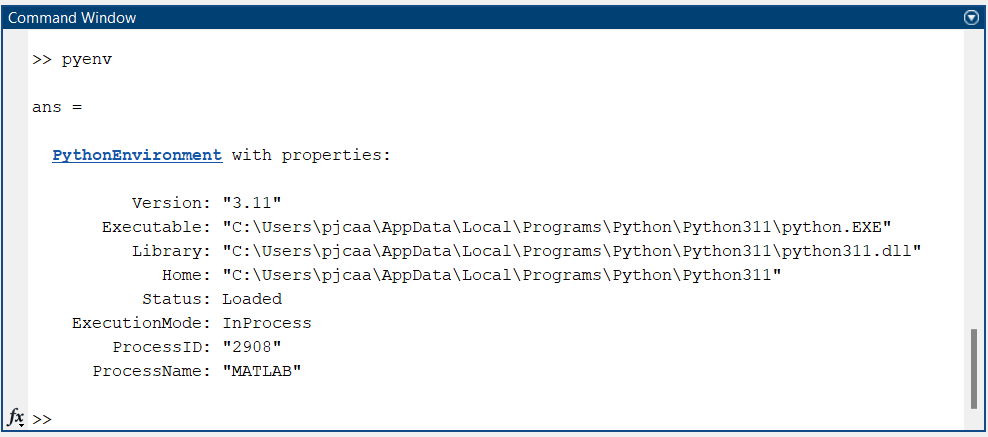
\includegraphics[width=0.85\textwidth]{Matlab_python}
	\caption{Terminal de comandos de Matlab con ejecución del comando pyversion.}
	\label{fig:Matlab_python}
\end{figure} 

\newpage
\subsubsection{Ejecución de algoritmos de Python desde Matlab}
Una vez comprobado que el entorno de trabajo de Matlab había cargado correctamente la versión de Python deseada, se procedió a verificar la capacidad de importar módulos de Python directamente en Matlab. Para ello, se realizó nuevamente un experimento de conexión y desconexión del Crazyflie. 

\vspace{5mm}
\begin{lstlisting}[caption=Algoritmo de prueba de conexión con Crazyflie., label=code:matlab_prueba1]
	import time
	import logging
	import cflib.crtp
	from cflib.crazyflie import Crazyflie
	
	def connect_crazyflie():
		cflib.crtp.init_drivers()
		logging.basicConfig(level=logging.CRITICAL)
		cf = Crazyflie(rw_cache='./cache')
		
		try:
			cf.open_link('radio://0/80/2M/E7E7E7E7E7')
			print(f"Crazyflie conectado.")
			time.sleep(5)  # Espera 5 segundos
			
		except Exception as e:
			print(f"Ocurrió un error al intentar conectar o durante la operación: {e}")
		
		finally:
			cf.close_link()
			print(f"Crazyflie desconectado.")

\end{lstlisting}

El código \ref{code:matlab_prueba1} corresponde a un script en Python con una función que realiza la conexión y desconexión del Crazyflie. Para realizar la llamada del script de Pyhton desde Matlab y ejecutar la función se utilizaron los siguientes comandos propios de Matlab:

\begin{verbatim}
	% Importa el archivo Python
	modulo = py.importlib.import_module('crazyflie_library_test');
	
	% Llama a la función desde MATLAB
	modulo.connect_crazyflie();
\end{verbatim}

El resultado obtenido se muestra en la Figura \ref{fig:Matlab_python2}, en donde se observa que en la consola de Matlab se mostraron los mensajes programados en el algoritmo de Python y se creó un objeto llamado módulo que internamente poseía las instancias de las librerías y objetos creados en el algortimo de Python. Lo que demostró que fue efectiva la ejecución e importación de algoritmos de Python directamente desde Matlab.

\vspace{5mm}
\begin{figure}[htbp]
	\centering
	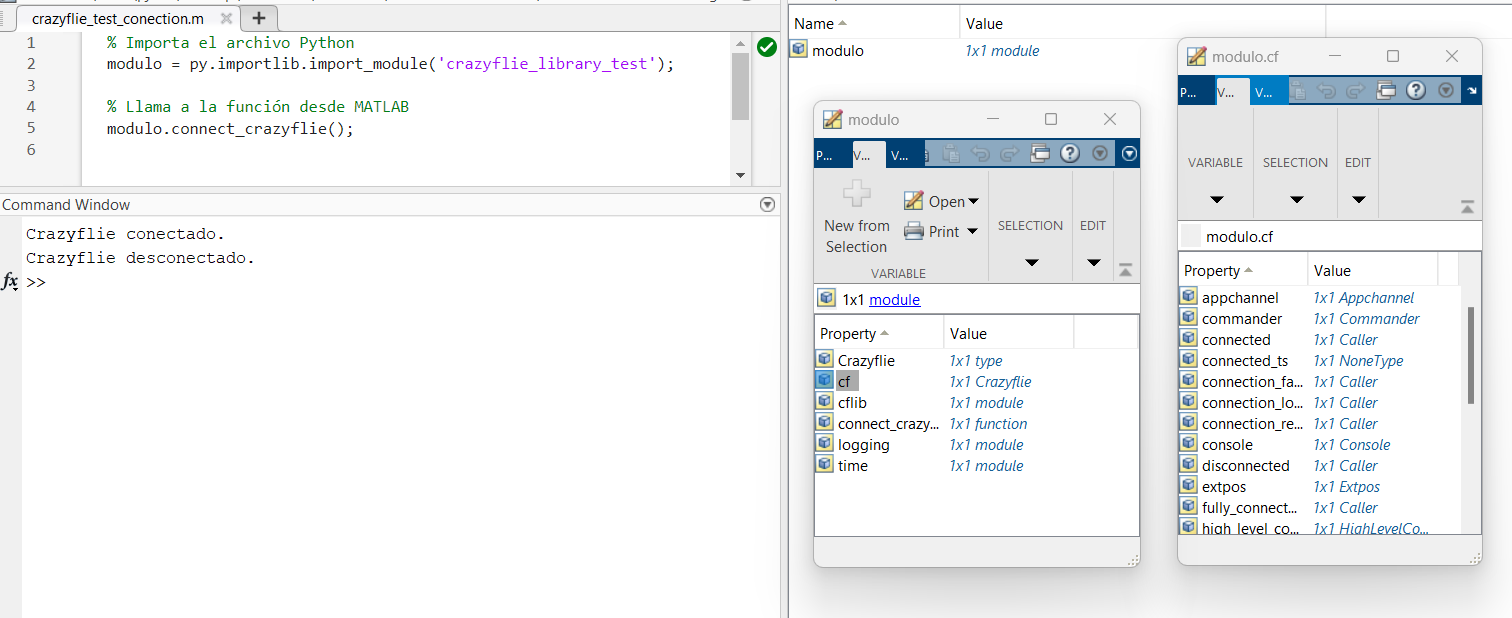
\includegraphics[width=0.9\textwidth]{Matlab_python2}
	\caption{Ejecución de script en Python de código \ref{code:prueba_conexion_crazyflie} desde Matlab.}
	\label{fig:Matlab_python2}
\end{figure} 

\subsection{Algoritmos de control en Python desde Matlab}
Una vez demostrada la correcta ejecución de algoritmos de Python desde Matlab, se desarrolló un conjunto de comandos en Matlab que permiten ejecutar funciones escritas en Python de forma directa y sencilla. Estos comandos actúan como funciones de Matlab que, internamente, llaman de manera individual a los módulos y funciones correspondientes en Python. De esta manera, es posible enviar comandos al Crazyflie sin la necesidad de interactuar directamente con Python, facilitando el uso de algoritmos de control y la realización de experimentos de vuelo complejos en el entorno conocido de Matlab.

\subsubsection{Comandos de conexión en Matlab}
\begin{itemize}
	\item crazyflie\_connect(uri)
	\item crazyflie\_disconnect(SyncCrazyflie)
\end{itemize}

\subsubsection{Comandos de lectura de variables en Matlab}
\begin{itemize}
	\item crazyflie\_get\_pose(SyncCrazyflie)
	\item crazyflie\_get\_pid\_values(SyncCrazyflie)
	\item crazyflie\_get\_pid\_x(SyncCrazyflie)
	\item crazyflie\_get\_pid\_y(SyncCrazyflie)
	\item crazyflie\_get\_pid\_z(SyncCrazyflie)
	\item crazyflie\_detect\_flow\_deck(SyncCrazyflie)
\end{itemize}

\subsubsection{Comandos de configuración de parámetros en Matlab}
\begin{itemize}
	\item crazyflie\_set\_position(SyncCrazyflie, x, y, z)
	\item crazyflie\_set\_pid\_values(SyncCrazyflie, p\_gains, i\_gains, d\_gains)
	\item crazyflie\_set\_pid\_x(SyncCrazyflie, P, I, D)
	\item crazyflie\_set\_pid\_y(SyncCrazyflie, P, I, D)
	\item crazyflie\_set\_pid\_z(SyncCrazyflie, P, I, D)
\end{itemize}

\subsubsection{Comandos de movimiento en Matlab}
\begin{itemize}
	\item crazyflie\_takeoff(SyncCrazyflie, height, duration)
	\item crazyflie\_land(SyncCrazyflie, height, duration)
	\item crazyflie\_move\_to\_position(SyncCrazyflie, x, y, z, velocity)
\end{itemize}
\vspace{5mm}
	
\subsection{Experimentos con algoritmos de control desde Matlab}
El desarrollo de los comandos de control en Matlab fue un proceso iterativo, ya que para cada comando desarrollado fue necesario realizar una serie de pruebas distintas para validar su funcionamiento bajo distintas condiciones. Una vez concluidos los comandos y verficado el funcionamiento individual, es posible realizar experimentos más complejos utilizando todos los comandos en conjunto. A continuación, se presentan algunos de los experimentos realizados:

\subsubsection{Experimento de despegue simple}
Este experimento consistió en un despegue básico, evaluando la estabilidad del dron durante la elevación y comprobando la capacidad de mantenerse en vuelo estacionario.
\vspace{5mm}
\begin{lstlisting}[caption=Algoritmo de experimento de despegue simple con Crazyflie en Matlab., label=code:prueba1_matlab]
	dron_id = 8; 
	crazyflie_1 = crazyflie_connect(dron_id);
	crazyflie_takeoff(crazyflie_1, 0.5, 2.5);
	crazyflie_land(crazyflie_1);
	crazyflie_disconnect(crazyflie_1);
\end{lstlisting}

\begin{figure}[htbp]
	\centering
	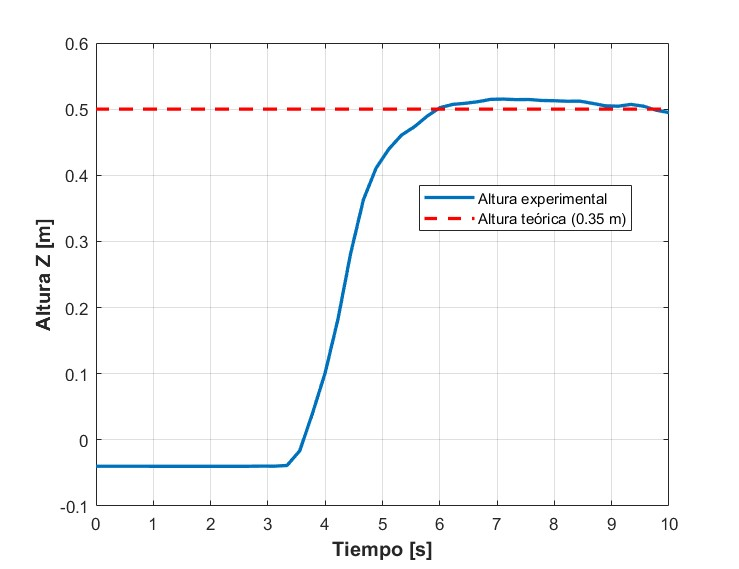
\includegraphics[width=0.65\textwidth]{takeoff}
	\caption{Gráfica de altura contra tiempo del experimento de despegue simple.}
	\label{fig:takeoff}
\end{figure} 

En la Figura \ref{fig:takeoff}, se muestra el comportamiento de vuelo para el experimento de despegue simple y evidencia el comportamiento esperado. Inicia en una altura aproximada de 0 metros y comienza a elevarse de manera progresiva hasta alcanzar la altura indicada de 0.5 metros. Este experimento se desarrolló con los valores normales para el controlador PID, por lo que vemos un comportamiento bastante estable y con error mínimo. 

\subsubsection{Experimento de despegue con modificación en el control PID de posición z}
Se realizó una modificación de los parámetros PID para el control en el eje Z durante el despegue, evaluando el impacto en la precisión y estabilidad del vuelo.
\vspace{5mm}
\begin{lstlisting}[caption=Algoritmo de experimento de despegue con modificación en el control PID de altura con Crazyflie en Matlab., label=code:prueba2_matlab]
	dron_id = 8;    
	crazyflie_1 = crazyflie_connect(dron_id);
	crazyflie_set_pid_z(crazyflie_1, 2.5, 1.5, 0.01);
	crazyflie_takeoff(crazyflie_1, 0.5, 2.5);
	crazyflie_land(crazyflie_1);
	crazyflie_disconnect(crazyflie_1);
\end{lstlisting}

\begin{figure}[htbp]
	\centering
	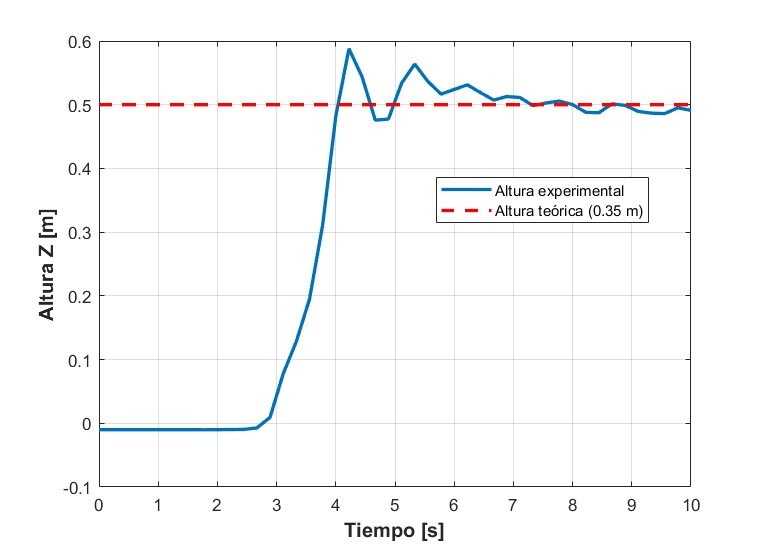
\includegraphics[width=0.65\textwidth]{takeoff_pid}
	\caption{Gráfica de altura contra tiempo del experimento de despegue con modificación de control PID de altura.}
	\label{fig:takeoff_pid}
\end{figure} 

En la gráfica de la Figura \ref{fig:takeoff_pid}, se muestra el despegue del dron Crazyflie con la modificación del control PID de altura. Tal como era esperado, se observa una variación en el comportamiento de vuelo del dron que, para el caso de los parámetros seleccionados, el comportamiento es un poco inestable. Esto se evidencia al ver que el vuelo presenta sobreimpulso al alcanzar la altura deseada, es decir, sobrepasa la altura y luego intenta estabilizarse. De esta forma, se validan las funciones de configuración de parámetros de los controladores PID de posición.

\subsubsection{Experimento de seguimiento de trayectoria circular}
En este experimento, se programó al Crazyflie para seguir una trayectoria circular.

\vspace{5mm}
\begin{lstlisting}[caption=Algoritmo de experimento de seguimiento de trayectoria circular con Crazyflie en Matlab., label=code:prueba4_matlab]
	circle_center = [0,0,0.5];
	N = 20;
	radio = 0.3;
	theta = linspace(0, 2*pi, N);  
	x = circle_center(1) + radio * cos(theta);
	y = circle_center(2) + radio * sin(theta);
	z = circle_center(3) * ones(1, N);
	
	dron_id = 8;    
	crazyflie_1 = crazyflie_connect(dron_id);
	crazyflie_takeoff(crazyflie_1, 0.3, 2.5); 
	for i = 1:N
		crazyflie_move_to_position(crazyflie_1, x(i), y(i), z(i), 0.2);
	end
	crazyflie_land(crazyflie_1);
	crazyflie_disconnect(crazyflie_1);
\end{lstlisting}

\begin{figure}[htbp]
	\centering
	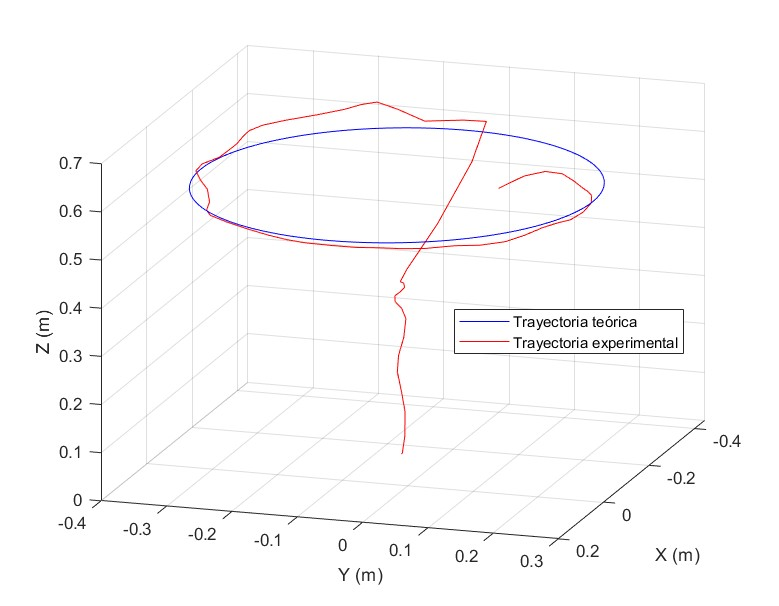
\includegraphics[width=0.65\textwidth]{Trayectoria1_FlowDeck}
	\caption{Gráfica 3D del seguimiento de trayectoria circular.}
	\label{fig:Trayectoria1_FlowDeck}
\end{figure} 

\newpage
\begin{figure}[htbp]
	\centering
	\begin{subfigure}[b]{0.4\textwidth}
		\centering
		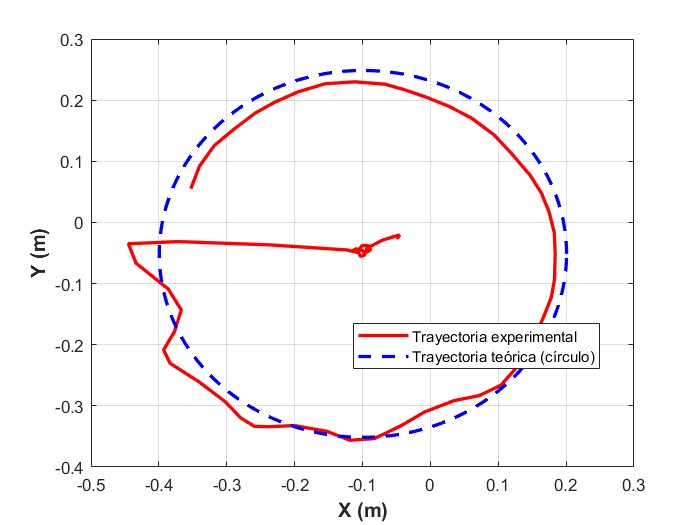
\includegraphics[width=\textwidth]{Trayectoria1_FlowDeck_xy}
	\end{subfigure}
	\hspace{0.01\textwidth} % Ajusta el espacio entre las imágenes
	\begin{subfigure}[b]{0.47\textwidth}
		\centering
		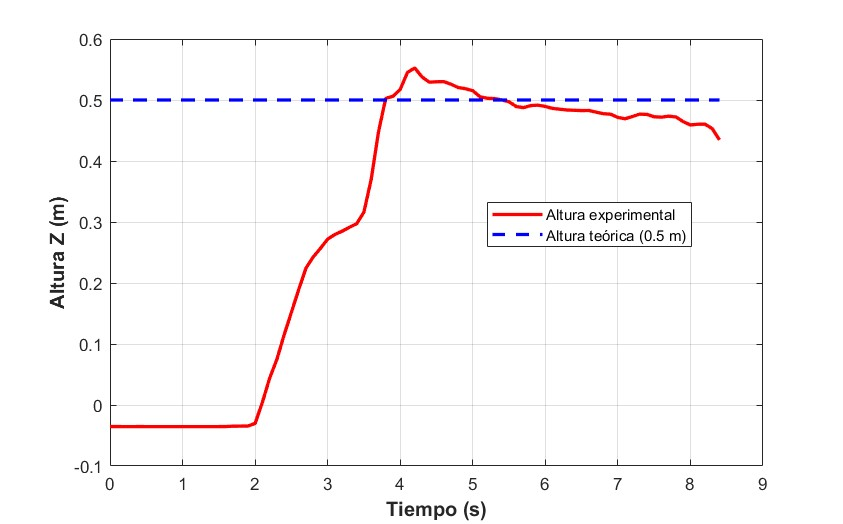
\includegraphics[width=\textwidth]{Trayectoria1_FlowDeck_z}
	\end{subfigure}
	\caption{Gráfica de posición X contra Y y gráfiza de altura contra tiempo para el seguimiento de trayectoria circular.}
	\label{fig:Trayectoria1_FlowDeck_xyz}
\end{figure}

Al analizar las gráficas mostradas en las Figuras \ref{fig:Trayectoria1_FlowDeck} y \ref{fig:Trayectoria1_FlowDeck_xyz}, se observa que el dron Crazyflie es capaz de realizar el seguimiento de las trayectorias generadas aunque no perfectamente. En la gráfica del plano X-Y, se observa que el dron experimenta desviaciones significativas en la trayectoria circular y en la gráfica de altura conta tiempo, se ve que el dron presenta una disminución progresiva de altura conforme pasa el tiempo. 

Las posibles fuentes de error incluyen limitaciones con el sensor Flow Deck, que puede verse afectado por la superficie de experimentación o la iluminación del entorno de pruebas. Aunque se intentó adaptar las condiciones del entorno para que fueran óptimas para su funcionamiento, parece que este aún presenta dificultades para posicionarse con precisión, lo que resulta en dificultades para mantener un seguimiento perfecto de la trayectoria generada. 

\newpage
\section{Fusión de sensores}
Derivado de los resultados obtenidos, se identificó que el comportamiento de vuelo podía ser mejorado de forma considerable al realizar una fusión de sensores con un sistema de posicionamiento absoluto. A raíz de ello, se intentó fusionar las lecturas de posicionamiento de la placa de expansión Flow Deck con los datos obtenidos a través del sistema de captura de movimiento del ecosistema Robotat.

Esto permitiría optimizar significativamente el rendimiento del dron, ya que las lecturas de posición relativa proporcionadas por la palca Flow Deck se complementarían con las lecturas absolutas del sistema MoCap, brindando al dron una referencia precisa de su posición dentro del entorno. Los datos de ambas fuentes serían procesados mediante el filtro extendido de Kalman para una estimación más exacta de su posición, mejorando considerablemente la precisión de vuelo del dron Crazyflie en el seguimiento de trayectorias.

\subsection{Sistema de captura de movimiento y funcionamiento desde Matlab}
El MoCap está compuesto por una red de cámaras que rastrean marcadores reflectivos adheridos a los objetos que se desean monitorear dentro del espacio controlado. Dichos marcadores permiten que el sistema calcule la posición y orientación exacta de los objetos en tiempo real respecto a una referencia absoluta. 

En el ecosistema Robotat, se utiliza una red TCP para la comunicación con el Mocap. Matlab es el software mayormente utilizado como panel de control en los laboratorios y experimentos de la universidad. Por lo tanto, es por medio de Matlab que se establece una conexión con el sistema MoCap para solicitar las poses de los marcadores reflectivos. A continuación, se listan las funciones principales para controlar el sistema:

\begin{itemize}
	\item \textbf{tcp\_obj = robotat\_connect()}: Esta función establece la conexión con la red TCP del ecosistema Robotat.
	\item \textbf{pose = robotat\_get\_pose(tcp\_obj, id\_agent)}: Solicita y devuelve la posición y orientación del marcador reflectivo especificado por id\_agent.
	\item \textbf{robotat\_disconnect(tcp\_obj)}: Finaliza la conexión con el sistema.
\end{itemize}

\subsubsection{Marcador reflectivo}
Un marcador reflectivo es un conjunto de pequeñas esferas reflectantes sujetadas sobre los cuerpos que se desean rastrear dentro del sistema. Estos marcadores están diseñados para reflejar luz emitida por las cámaras, permitiendo que el \textit{software} reconozca su posición en el espacio con alta precisión.

Para llevar a cabo la fusión de sensores de la placa Flow Deck y el sistema MoCap en el dron Crazyflie, es necesario colocar un marcador reflectivo sobre el dron. Para ello, se desarrollaron distintos prototipos de marcador que pudieran colocarse en la parte superior del Crazyflie sin afectar a las hélices y que fuera fácilmente perceptible por el sistema MoCap.

\begin{figure}[htbp]
	\centering
	\begin{subfigure}[b]{0.35\textwidth}
		\centering
		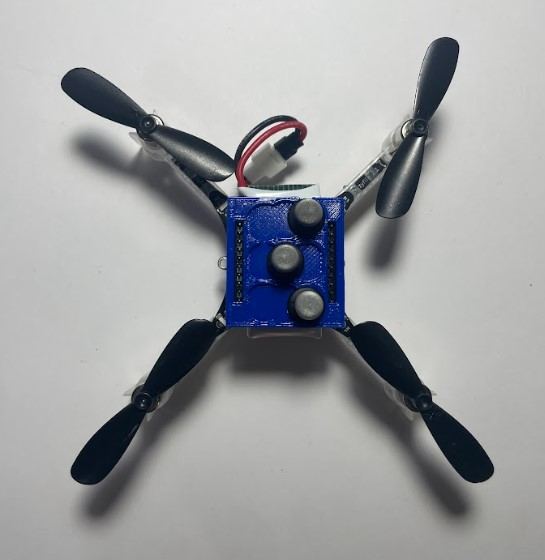
\includegraphics[width=\textwidth]{Crazyflie_marker_1}
	\end{subfigure}
	\hspace{0.01\textwidth} % Ajusta el espacio entre las imágenes
	\begin{subfigure}[b]{0.38\textwidth}
		\centering
		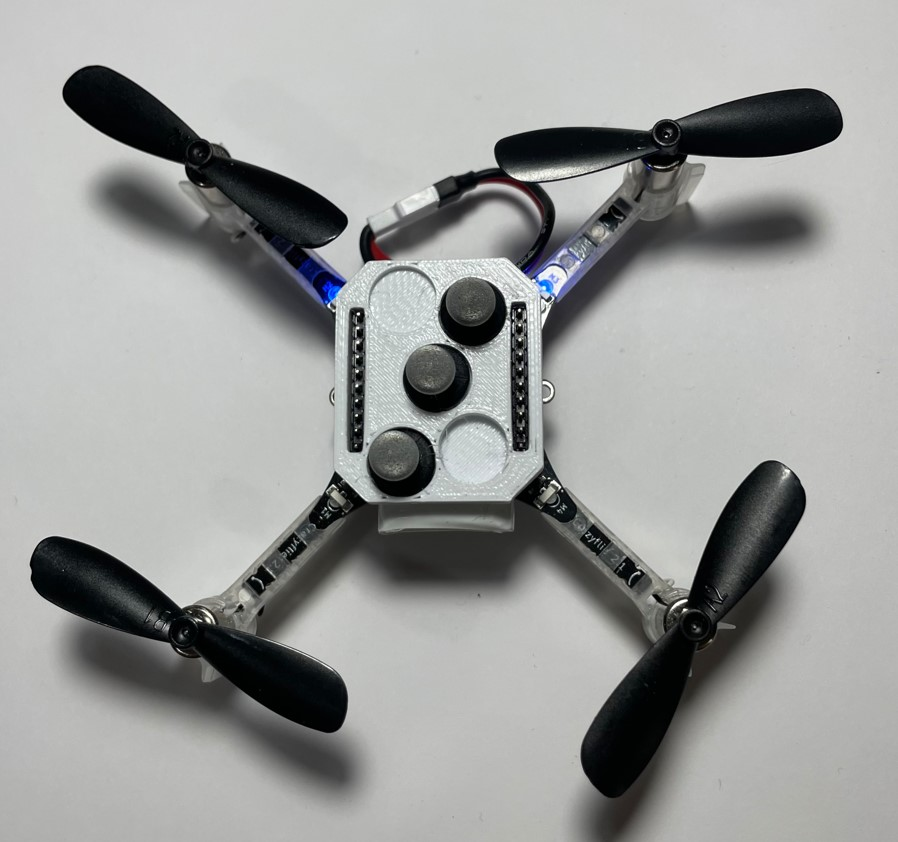
\includegraphics[width=\textwidth]{Crazyflie_marker_2}
	\end{subfigure}
	\caption{Versiones iniciales del marker para Crazyflie.}
	\label{fig:Markers_primeras_versiones}
\end{figure}

En la Figura \ref{fig:Markers_primeras_versiones} se muestran las primeras versiones desarrolladas para sujetar a las esferas reflectantes que conformarían al marcador reflectivo del dron Crazyflie. Sin embargo, presentaron cirtas dificultades al utilizar el sistema MoCap, pues en ocasiones no se registraban lecturas del cuerpo rígido. Un factor que causo esto fue que las esferas eran sobrepuestas en agujeros pero sin sostenerlas de forma definitiva, lo que ocasionaba que se movimieran milimétricamente. También, se cree que la poca distancia entre esferas dificultaba el reconocimiento del cuerpo rígido en sistema MoCap.
\vspace{5mm}
\begin{figure}[htbp]
	\centering
	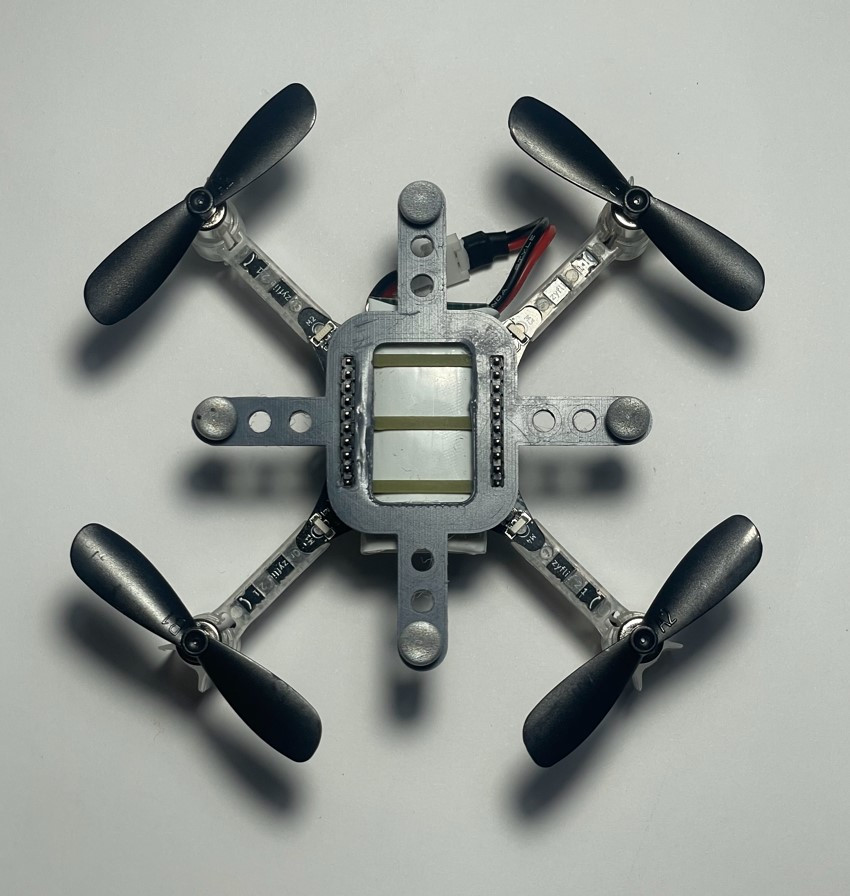
\includegraphics[width=0.4\textwidth]{Crazyflie_marker_3}
	\caption{Versión final de marcador reflectivo para dron Crazyflie.}
	\label{fig:Marker_version_final}
\end{figure} 

Tras observar estos factores, se realizó el diseño final del marcador para el dron Crazyflie, mostrado en la Figura \ref{fig:Marker_version_final}. Este dispone de agujeros para sujetar a las esferas mediante tornillos M3, de forma que la posición de estas queda totalmente rígida. Además, se utilizó una distancia considerablemente mayor entre esferas reflectivas y se añadió una esfera extra para disminuir la pérdida de reconocimiento por parte del sistema MoCap.


\subsection{Implementación de fusión de sensores}
Para la implementación de la fusión de sensores previamente descrita, se utilizó el submódulo extpos de la clase Crazyflie en la librería cflib de Python. Los datos obtenidos del sistema MoCap se enviaron mediante las funciones de este submódulo para actualizar la posición absoluta del dron, por medio del comando crazyflie\_set\_pose en Matlab. 

\subsubsection{Función de actualización de posición externa en Python}
Se desarrolló una función en Matlab que solicita las lecturas del sistema MoCap a través de la red TCP del ecosistema Robotat \ref{code:robotat_}, tal cual lo hace la función robotat\_get\_pose. Esta función también emplea del comando de actualización de posición del dron Crazyflie para completar la fusión de lecturas.

\subsubsection{Event Callback en Matlab}
Se intentó desarrollar una rutina de Event CallBack en Matlab, en la cual el evento sería la recepción de datos desde la red TCP. Sin embargo, debido a la naturaleza del sistema Robotat, que opera bajo un esquema de solicitud y recepción de información, no fue posible implementar un evento conntinuo, ya que la red TCP no envía datos de manera constante sin una solicitud previa.

\subsubsection{Sistema de corrección de posición}
Debido a la imposibilidad de implementar una fusión continua de datos en tiempo real, los datos obtenidos del sistema MoCap se utilizan de manera periódica para corregir la posición del dron. Esto compensa las desviaciones que ocurren durante el uso de la placa Flow Deck, mejorando la precisión general del dron dentro del ecosistema Robotat. 

\subsection{Pruebas de algoritmos de control con fusión de sensores desde Matlab}
Acá se describirán las pruebas ha realizarse con la mezcla de lecturas de posición...

\newpage
\begin{lstlisting}[caption=Función para actualización de posición absoluta del Crazyflie desde Matlab., label=code:robotat_]
	function robotat_update_crazyflie_position(scf, tcp_obj, agents_ids)
		max_retries = 3; 
		for attempt = 1:max_retries
			try
				timeout_count = 0;
				timeout_in100ms = 1 / 0.1;
				read(tcp_obj); 				
				if((min(agents_ids) > 0) && (max(agents_ids) <= 100))
					s.dst = 1; 
					s.cmd = 1; 
					s.pld = round(agents_ids);
					write(tcp_obj, uint8(jsonencode(s)));  
					while((tcp_obj.BytesAvailable == 0) && (timeout_count < timeout_in100ms))
						timeout_count = timeout_count + 1;
						pause(0.1);
					end					
					if(timeout_count == timeout_in100ms)
						disp('ERROR: Could not receive data from server.');
						continue;
					else
						absolute_position = jsondecode(char(read(tcp_obj)));
						absolute_position = reshape(absolute_position, [7, numel(agents_ids)])';						
						x = absolute_position(1);
						y = absolute_position(2);
						z = absolute_position(3);						
						module_name = 'crazyflie_python_commands'; 
						py_module = py.importlib.import_module(module_name);  
						py.importlib.reload(py_module);						
						try
							py_module.set_position(scf, x, y, z);
						catch ME
							error('Error using crazyflie_python_commands>set_position: %s', ME.message);
						end 						
						break;
					end
				else
					disp('ERROR: Invalid ID(s).');
					return;
				end			
			catch ME
				disp(['ERROR: ', ME.message]);
				if attempt == max_retries
					disp('Max retries reached, exiting.');
				else
					disp('Retrying...');
				end
			end
		end
	end
\end{lstlisting}

\newpage
\section{Simuladores para dron Crazyflie 2.1}
Los simuladores son herramientas cruciales en el desarrollo y prueba de algoritmos que involucran a agentes robóticos, ya que permiten simular entornos reales sin poner en riesgo el \textit{hardware} o a los experimentadores. Para el dron Crazyflie 2.1, existen algunos simuladores que permiten modelar su comportamiento en distintos escenarios, brindando un entorno seguro y flexible para experimentar con algoritmos de control y planificación de trayectorias. A continuación, se describen algunos de los simuladores utilizados que cuentan con modelos del dron Crazyflie 2.1.

\subsection{Webots}
Webots es un simulador de robots de código abierto que permite simular una amplia variedad de agentes robóticos en entornos tridimensionales. Desarrollado por Cyberbotics, Webots está diseñado para ser flexible y permite la programación de robots utilizando lenguajes como Python, C++, Java y Matlab. Es ampliamente utilizado en entornos académicos y de investigación por su capacidad de simular entornos complejos-

\subsubsection{Modelo de dron Crazyflie}
En Webots, existe un modelo del dron Crazyflie 2.1 que simula su comportamiento dinámico. Este modelo incluye herramientas para controlar al dron mediante scripts de control, lo que permite a los usuarios programar su movimiento, maniobras y experimentos con facilidad. Además, ofrece la posibilidad de integrar sensores virtuales como cámaras, IMUs y sensores de distancias.

\begin{figure}[htbp]
	\centering
	\includegraphics[width=0.85\textwidth]{Webots1}
	\caption{Simulación de modelo Crazyflie 2.1 en Webots.}
	\label{fig:Webots1}
\end{figure} 


\subsubsection{Alcance de simulaciones}


%\subsection{gym-pybullet-drones}
%Párrafo explicando qué es gym-pybullet-drones.
%\subsubsection{Modelo de dron Crazyflie}
%Párrafo explicando el modelo y herramientas disponibles para el dron Crazyflie en el simulador.
%\subsubsection{Alcance de simulaciones}

%\subsection{Nvidia Isaac}
%Párrafo explicando qué es Nvidia Isaac.
%\subsubsection{Modelo de dron Crazyflie}
%Párrafo explicando el modelo y herramientas disponibles para el dron Crazyflie en el simulador.
%\subsubsection{Alcance de simulaciones}
% ------------------------------------------------------------------------------
% CAPÍTULO 9 -------------------------------------------------------------------
% ------------------------------------------------------------------------------
\chapter{Manual de usuario y guías de laboratorio desarrolladas}
En este capítulo se presenta finalmente la elaboración de un manual de usuario e instalación de herramientas para el uso del Crazyflie 2.1 con la placa Flow Deck integrada. Asimismo, se presentan los experimentos y el desarrollo de las guías de laboratorio diseñados para los cursos de Sistemas de Control 1 y Robótica 1.

\section{Manual de usuario de Crazyflie con la placa Flow Deck}
Para cualquier equipo de laboratorio es fundamental contar con una documentación adecuada y un manual de uso que se revise previamente. Esto asegura que los usuarios comprendan cómo operar el equipo de manera segura y eficiente. En el caso del dron Crazyflie 2.1 y su placa de expansión Flow Deck, resulta indispensable disponer de un manual detallado que documente la información clave para su uso correcto durante las prácticas de laboratorio.

\subsection{Descripción}
Este manual está diseñado para guiar al usuario en el uso del dron Crazyflie 2.1 con la placa de expansión Flow Deck integrada. Proporciona instrucciones claras sobre cómo ensamblar, configurar, y operar el dron, así como las recomendaciones para el manejo de sus componentes. Además, incluye pasos detallados para la instalación de las herramientas de \textit{software} necesarias y cómo realizar pruebas básicas para verificar su funcionamiento.

\subsection{Objetivos}
\begin{itemize}
	\item Familiarizarse con el funcionamiento básico del dron Crazyflie 2.1 y la placa Flow Deck.
	\item Validar el ensamble y la instalación de la placa Flow Deck.
	\item Aprender a conectar el dron a su ordenador mediante el dispósitivo Crazyradio.
	\item Configurar las dependencias y librerías de \textit{software} necesarias para programar y controlar el dron desde Python.
	\item Realizar pruebas de conexión y verificación del funcionamiento de la placa Flow Deck, asegurando que el dron esté listo para su uso en experimentos de laboratorio.
\end{itemize}

\subsection{Prueba piloto}
\subsubsection{Descripción y condiciones de la prueba}
Acá se describirá una descripción y las condiciones en las que se desarrollará la prueba piloto.

\subsubsection{Material y Equipo Necesario}
A continuación, se presenta el listado de materiales y equipo necesarios para seguir los pasos de este manual:

\begin{itemize}
	\item Dron Crazyflie 2.1 ensamblado.
	\item Placa de expansión Flow Deck.
	\item Dispositivo Crazyradio.
	\item Ordenador con Windows 10/11.
\end{itemize}

\subsubsection{Resulados y recomendaciones}
Acá se detallarán los resultados de la prueba junto con las recomendaciones dadas. 

\newpage
\section{Guía de laboratorio para Sistemas de Control 1: Control de altura del dron Crazyflie 2.1}
\subsection{Descripción}
Este laboratorio utiliza el dron Crazyflie 2.1 como planta de estudio para implementar y ajustar controladores PID que permitan controlar su altura de vuelo. En primer lugar, los estudiantes realizarán simulaciones en MATLAB para modelar el comportamiento del dron bajo diferentes condiciones. Luego, realizarán experimentos con el dron físico, ajustando los parámetros del controlador PID y utilizando el sistema de captura de movimiento del laboratorio CIT-116 para medir y analizar su desempeño real.

\subsection{Objetivos}
\begin{itemize}
	\item Estudiar el funcionamiento del controlador PID aplicado al dron Crazyflie 2.1, analizando cómo los parámetros afectan la estabilidad y precisión del control de altura.
	\item Implementar y ajustar controladores PID en MATLAB para simular y experimentar con el control de altura del dron.
	\item Comparar los resultados obtenidos en simulaciones con los resultados obtenidos mediante la experimentación en el dron físico.
	\item Familiarizarse con el sistema de captura de movimiento del ecosistema Robotat para registrar los movimientos del dron y evaluar su rendimiento.
\end{itemize}

\subsection{Prueba piloto}
\subsubsection{Descripción y condiciones de la prueba}
Acá se describirá una descripción y las condiciones en las que se desarrollará la prueba piloto.

\subsubsection{Material y Equipo Necesario}
A continuación, se presenta el listado de materiales y equipo necesarios para seguir los pasos de este manual:

\begin{itemize}
	\item Dron Crazyflie 2.1 con la placa de expansión Flow Deck integrada.
	\item Dispositivo Crazyradio.
	\item Ordenador con Windows 10/11 con Matlab y Pyhton instalados.
	\item Paquete de herramientas de software descargado.
	\item Sistema de Captura de Movimiento del ecosistema Robotat del laboratorio CIT-116.
\end{itemize}

\subsubsection{Resulados y recomendaciones}
Acá se detallarán los resultados de la prueba junto con las recomendaciones dadas. 

\newpage
\section{Guía de laboratorio para Robótica 1: Generación y seguimiento de trayectorias con Crazyflie 2.1}
\subsection{Descripción}
En esta práctica usted aprenderá a utilizar a los drones Crazyflie 2.1 con una placa de posicionamiento relativo (Flow Deck). También, hará uso nuevamente del sistema de captura de movimiento óptico. Luego, empleará rutinas básicas en MATLAB para obtener la pose absoluta del cuerpo rígido Crazyflie para otorgarle sentido de posición absoluta al dron y finalmente realizar un experimento de seguimiento de trayectoria a través de una ruta de obstáculos.

\subsection{Objetivos}
\begin{itemize}
	\item Familiarizarse con los agentes robóticos móviles Crazyflie 2.1.
	\item Comprender a la diferencia entre un sistema de posicionamiento relativo y un sistema de posicionamiento absoluto.
	\item Familiarizarse con el sistema de captura de movimiento del ecosistema Robotat para registrar los movimientos del dron y evaluar su rendimiento.
	\item Generar trayectorias y ejecutarlas con los drones Crazyflie 2.1.
\end{itemize}

\subsection{Prueba piloto}
\subsubsection{Descripción y condiciones de la prueba}
Acá se describirá una descripción y las condiciones en las que se desarrollará la prueba piloto.

\subsubsection{Material y Equipo Necesario}
A continuación, se presenta el listado de materiales y equipo necesarios para seguir los pasos de este manual:

\begin{itemize}
	\item Dron Crazyflie 2.1 con la placa de expansión Flow Deck integrada.
	\item Dispositivo Crazyradio.
	\item Ordenador con Windows 10/11 con Matlab y Pyhton instalados.
	\item Paquete de herramientas de software descargado.
	\item Sistema de Captura de Movimiento del ecosistema Robotat del laboratorio CIT-116.
\end{itemize}

\subsubsection{Resulados y recomendaciones}
Acá se detallarán los resultados de la prueba junto con las recomendaciones dadas. 

\fi

% CONCLUSIONES
% ------------------------------------------------------------------------------
\ifdefined\CAPconclusiones
	\newpage
	\chapter{Conclusiones}
	\ifdefined\parpordefecto
		\defaultparformat{k-conclusiones}
	\else
		\begin{itemize}
	\item Se realizó la integración de la placa de expansión Flow Deck en el dron Crazyflie 2.1, validando su funcionamiento mediante un conjunto de pruebas de vuelo y posicionamiento simples. En el proceso, se identificó una superifice con las condiciones para el correcto funcionamiento de los sensores presentes en la placa Flow Deck.
	
	\item Se desarrollaron herramientas de \textit{software} para controlar y monitorear de forma simple al dron Crazyflie con la placa Flow Deck incorporada. Estas funciones permiten ejecutar desde experimentos simples de despegue, hasta seguimientos de trayectorias.
	
	\item Se desarrolló un manual de usuario para el dron Crazyflie 2.1 con la placa de expansión Flow Deck integrada, proporcionando a los usuarios una guía detallada sobre el ensamble, configuración y manejo del dron. 	
	
	\item Se desarrolló una guía de laboratorio diseñada para el curso de Sistemas de Control 1, donde se utilizó al Crazyflie 2.1 con la placa Flow Deck para evaluar el comportamiento de vuelo al modificar las constantes del controlador PID de altura del dron.
	
	\item Se desarrolló una guía de laboratorio diseñada para el curso de Robótica 1, donde se utilizó al Crazyflie 2.1 con la placa Flow Deck para la generación y seguimiento de trayectorias a través de una pista de obstáculos sobre el ecosistema de investigación Robotat.
\end{itemize}

	\fi
\fi

% RECOMENDACIONES
% ------------------------------------------------------------------------------
\ifdefined\CAPrecomendaciones
	\newpage
	\chapter{Recomendaciones}
	\ifdefined\parpordefecto
		\defaultparformat{l-recomendaciones}
	\else
		
\begin{itemize}
	\item Se recomienda adquirir otras placas de expansión para ampliar las capacidades del dron Crazyflie. En particular, la placa de expansión MultiRanger axpandiría las capacidades del dron para detectar obstáculos, permitiendo que el dron detecte y evite obstáculos de manera autónnoma.
	
	\item Se recomienda instalar una red de protección alrededor de la mesa de trabajo del ecosistema Robotat con el fin de evitar accidentes que dañen a los usuarios, drones o equipo de laboratorio. 
	
	\item Se sugiere modificar el protocolo de comunicación del ecosistema Robotat con el fin de poder implementar una fusión de sensores más eficiente, al habilitar la posibilidad de desarrollar una rutina de posicionamiento absoluto mediante una función callback basada en eventos. 
\end{itemize}

	\fi
\fi

% BIBLIOGRAFÍA
% ------------------------------------------------------------------------------
\ifdefined\CAPbibliografia
	\newpage
    \cleardoublepage\phantomsection
	\chapter{\bibname}
    \printbibliography[heading=none]
\fi

% ANEXOS
% ------------------------------------------------------------------------------
\ifdefined\CAPanexos
	\newpage
	\chapter{Anexos}
	\ifdefined\parpordefecto
		\defaultparformat{n-anexos}
	\else
		\section{Repositorio en GitHub}
Puede acceder al repositorio en Github por medio del siguiente enlace: \url{https://github.com/PabloCaal/Crazyflie-Matlab-Python}

\section{Manual de usuario para Crazyflie 2.1 con la placa de expansión Flow Deck}
Puede acceder al documento del manual de usuario por medio del siguiente enlace: \url{https://drive.google.com/file/d/157fDCxXf_BLKTRiDAqIZCCapgSy8fdp2/view?usp=sharing}

\section{Laboratorio 1: Control PID de altura}
Puede acceder al documento del laboratorio 1 por medio del siguiente enlace: \url{https://drive.google.com/file/d/1cBeLzd2d4w1BNKShUpOJaZk3qm76pnpr/view?usp=sharing}

\section{Laboratorio 2: Seguimiento de trayectorias}
Puede acceder al documento del laboratorio 2 por medio del siguiente enlace: \url{https://drive.google.com/file/d/110EhRG25IjRaHUYy3AXFovrk0BIy7Ew8/view?usp=sharing}

\newpage
\section{Funciones de control desarrolladas en Python}
\subsection{Función connect}
\begin{lstlisting}[caption=Función en Python para establecer la conexión con Crazyflie., label=code:funcion_connect]
	def connect(uri):
		try:        
			scf = SyncCrazyflie(uri, cf=Crazyflie(rw_cache='./cache'))
			scf.open_link()
			print(f"Connection to Crazyflie established successfully.")
			sys.stdout.flush()
			return scf
			
		except Exception as e:
			if 'Cannot find a Crazyradio Dongle' in str(e):
				print(f"Error: Crazyradio Dongle not found. Ensure the dongle is connected properly.")
			elif 'Connection refused' in str(e):
				print(f"Error: Connection to Crazyflie was refused. Check if the Crazyflie is powered on and in range.")
			else:
				print(f"General error occurred while trying to connect to Crazyflie. Error details: {str(e)}")
\end{lstlisting}

\subsection{Función disconnect}
\begin{lstlisting}[caption=Función en Python para cerrar la conexión con Crazyflie., label=code:funcion_disconnect]
	def disconnect(scf):
		try:
			if scf:
				scf.close_link()
				print(f"Successfully disconnected from Crazyflie.")
			else:
				print(f"Error: Invalid SyncCrazyflie object. No connection to close.")
				
		except Exception as e:
			print(f"Error: An issue occurred while disconnecting from Crazyflie. Error details: {str(e)}")
\end{lstlisting}

\newpage
\subsection{Función get\_pose}
\begin{lstlisting}[caption=Función en Python para obtener la pose actual del Crazyflie., label=code:funcion_get_pose]
	def get_pose(scf):
		try:
			# Set up the log configuration to get position and orientation data
			pose_log_config = LogConfig(name='Pose', period_in_ms=100)
			pose_log_config.add_variable('stateEstimate.x', 'float')
			pose_log_config.add_variable('stateEstimate.y', 'float')
			pose_log_config.add_variable('stateEstimate.z', 'float')
			pose_log_config.add_variable('stateEstimate.roll', 'float')
			pose_log_config.add_variable('stateEstimate.pitch', 'float')
			pose_log_config.add_variable('stateEstimate.yaw', 'float')
			pose = {'x': 0.0, 'y': 0.0, 'z': 0.0, 'roll': 0.0, 'pitch': 0.0, 'yaw': 0.0}
			new_data = Event()
			
			def pose_callback(timestamp, data, logconf):
				pose['x'] = data['stateEstimate.x']
				pose['y'] = data['stateEstimate.y']
				pose['z'] = data['stateEstimate.z']
				pose['roll'] = data['stateEstimate.roll']
				pose['pitch'] = data['stateEstimate.pitch']
				pose['yaw'] = data['stateEstimate.yaw']
				new_data.set()
			
			pose_log_config.data_received_cb.add_callback(pose_callback)
			
			try:
				existing_configs = scf.cf.log.log_blocks
				for config in existing_configs:
					if config.name == 'Pose':
						config.stop()
						config.delete()
						
			except AttributeError:
				pass  
				
			scf.cf.log.add_config(pose_log_config)
			pose_log_config.start()
			new_data.wait()
			pose_log_config.stop()
			print(f"Pose retrieved successfully")
			print(f"x: {pose['x']:.2f}, y: {pose['y']:.2f}, z: {pose['z']:.2f}, roll: {pose['roll']:.2f}, pitch: {pose['pitch']:.2f}, yaw: {pose['yaw']:.2f}")
			return [pose['x'], pose['y'], pose['z'], pose['roll'], pose['pitch'], pose['yaw']]
		
		except Exception as e:
			print(f"ERROR: An error occurred while retrieving the pose: {str(e)}")
\end{lstlisting}

\newpage
\subsection{Función get\_pid\_values}
\begin{lstlisting}[caption=Función en Python para obtener los valores de todos los PID de posición del Crazyflie., label=code:funcion_get_pid_values]
	def get_pid_values(scf):
		try:
			pid_values = {
				'X': [
				float(scf.cf.param.get_value('posCtlPid.xKp')),
				float(scf.cf.param.get_value('posCtlPid.xKi')),
				float(scf.cf.param.get_value('posCtlPid.xKd'))],
				'Y': [
				float(scf.cf.param.get_value('posCtlPid.yKp')),
				float(scf.cf.param.get_value('posCtlPid.yKi')),
				float(scf.cf.param.get_value('posCtlPid.yKd'))],
				'Z': [
				float(scf.cf.param.get_value('posCtlPid.zKp')),
				float(scf.cf.param.get_value('posCtlPid.zKi')),
				float(scf.cf.param.get_value('posCtlPid.zKd'))]
			}
			print("PID values for X axis: P={:.2f}, I={:.2f}, D={:.2f}".format(pid_values['X'][0], pid_values['X'][1], pid_values['X'][2]))
			print("PID values for Y axis: P={:.2f}, I={:.2f}, D={:.2f}".format(pid_values['Y'][0], 	pid_values['Y'][1], pid_values['Y'][2]))
			print("PID values for Z axis: P={:.2f}, I={:.2f}, D={:.2f}".format(pid_values['Z'][0], 	pid_values['Z'][1], pid_values['Z'][2]))
			return pid_values
		
		except Exception as e:
			print(f"ERROR: An error occurred during the pid values lecture: {str(e)}")
\end{lstlisting}

\subsection{Función get\_pid\_x}
\begin{lstlisting}[caption=Función en Python para obtener un PID de posición específico del Crazyflie., label=code:funcion_get_pid_x]
	def get_pid_x(scf):
		try:
			pid_x = {
				'P': float(scf.cf.param.get_value('posCtlPid.xKp')),
				'I': float(scf.cf.param.get_value('posCtlPid.xKi')),
				'D': float(scf.cf.param.get_value('posCtlPid.xKd'))
			}
			print("PID values for X axis: P = {:.2f}, I = {:.2f}, D = {:.2f}".format(pid_x['P'], pid_x['I'], 	pid_x['D']))
			return pid_x
		
		except Exception as e:
			print(f"ERROR: An error occurred while retrieving the PID values for X axis: {str(e)}")
\end{lstlisting}

\newpage
\subsection{Función detect\_flow\_deck}
\begin{lstlisting}[caption=Función en Python para detectar la placa Flow Deck en Crazyflie., label=code:funcion_detect_flow_deck]
	def detect_flow_deck(scf):
		try:
			flow_deck_detected = scf.cf.param.get_value('deck.bcFlow2')
			if flow_deck_detected == '1':
				print(f"Flow Deck detected successfully.")
				return 1
			else:
				print(f"Flow Deck not detected. Please verify that it is installed properly.")
				return 0
		
		except Exception as e:
			print(f"Error: An issue occurred while detecting the Flow Deck. Error details: {str(e)}")
\end{lstlisting}

\subsection{Función set\_position}
\begin{lstlisting}[caption=Función en Python para actualizar la posición del estimador del Crazyflie., label=code:funcion_set_position]
	def set_position(scf, x, y, z):
		try:
			if not all(isinstance(coord, (int, float)) for coord in [x, y, z]):
				print(f"ERROR: Input values invalids.")
			scf.cf.extpos.send_extpos(x, y, z)
			time.sleep(0.01)
			print(f"Absolute position successfully set.")
		
		except Exception as e:
			print(f"ERROR: An error occurred during the position update: {str(e)}")
\end{lstlisting}

\subsection{Función set\_pid\_x}
\begin{lstlisting}[caption=Función en Python para configurar a un PID de posición específico del Crazyflie., label=code:funcion_set_pid_x]
	def set_pid_x(scf, P, I, D):
		try:      
			scf.cf.param.set_value('posCtlPid.xKp', P)
			scf.cf.param.set_value('posCtlPid.xKi', I)
			scf.cf.param.set_value('posCtlPid.xKd', D)
			print(f"Successful PID modification.")
		
		except Exception as e:
			print(f"ERROR: An error occurred during the PID modification: {str(e)}")
\end{lstlisting}

\newpage
\subsection{Función set\_pid\_values}
\begin{lstlisting}[caption=Función en Python para configurar todos los PID de posición del Crazyflie., label=code:funcion_set_pid_values]
	def set_pid_values(scf, p_gains, i_gains, d_gains):
		try:       
			scf.cf.param.set_value('posCtlPid.xKp', p_gains['X'])
			scf.cf.param.set_value('posCtlPid.xKi', i_gains['X'])
			scf.cf.param.set_value('posCtlPid.xKd', d_gains['X'])
			scf.cf.param.set_value('posCtlPid.yKp', p_gains['Y'])
			scf.cf.param.set_value('posCtlPid.yKi', i_gains['Y'])
			scf.cf.param.set_value('posCtlPid.yKd', d_gains['Y'])
			scf.cf.param.set_value('posCtlPid.zKp', p_gains['Z'])
			scf.cf.param.set_value('posCtlPid.zKi', i_gains['Z'])
			scf.cf.param.set_value('posCtlPid.zKd', d_gains['Z'])
			print(f"Successful PID modification.")
		
		except Exception as e:
			print(f"ERROR: An error occurred during the PID modification: {str(e)}")
\end{lstlisting}

\subsection{Función takeoff}
\begin{lstlisting}[caption=Función en Python para despegar al Crazyflie., label=code:funcion_takeoff]
	def takeoff(scf, height = 0.3, duration = 1.0):
		try:
			position = get_pose(scf)
			current_z = position[2]  
			if current_z > 0.1:
				print(f"The Crazyflie was already in the air.")
				return 0
			commander = HighLevelCommander(scf.cf)
			commander.takeoff(absolute_height_m=height, duration_s=duration)
			time.sleep(duration)
			print(f"Takeoff completed successfully")
		
		except Exception as e:
			print(f"ERROR: An error occurred during takeoff: {str(e)}")
\end{lstlisting}

\newpage
\subsection{Función land}
\begin{lstlisting}[caption=Función en Python para aterrizar al Crazyflie., label=code:funcion_land]
	def land(scf, height = 0.0, duration = 2.0):
		try:
			position = get_pose(scf)
			current_z = position[2]  
			if current_z <= 0.1:
				print(f"The Crazyflie was already on the ground.")
				return 0
			commander = HighLevelCommander(scf.cf)
			commander.land(absolute_height_m=height, duration_s=duration)
			time.sleep(duration)
			commander.stop()
			print(f"Landing completed successfully.")
		
		except Exception as e:
			print(f"ERROR: An error occurred during landing: {str(e)}")
\end{lstlisting}

\subsection{Función move\_to\_position}\begin{lstlisting}[caption=Función en Python para enviar a una posición específica al Crazyflie., label=code:funcion_move_to_position]
	def move_to_position(scf, x, y, z, velocity = 1.0):
		try:
			commander = scf.cf.high_level_commander
			current_position = get_pose(scf)
			current_x, current_y, current_z = current_position[0], current_position[1], current_position[2]
			distance = ((x - current_x)**2 + (y - current_y)**2 + (z - current_z)**2)**0.5
			duration = distance / velocity
			commander.go_to(x, y, z, yaw=0.0, duration_s=duration)
			time.sleep(duration)
			print(f"Position command completed successfully")
		
		except Exception as e:
			print(f"ERROR: An error occurred during moving to position: {str(e)}")
\end{lstlisting}
	\fi
\fi

% GLOSARIO
% ------------------------------------------------------------------------------
\ifdefined\CAPglosario
	\newpage
	\chapter{Glosario}
	\ifdefined\parpordefecto
		\defaultparformat{o-glosario}
	\else
		\input{o-glosario}
	\fi
\fi

\end{document}